\documentclass[twoside]{book}

% Packages required by doxygen
\usepackage{fixltx2e}
\usepackage{calc}
\usepackage{doxygen}
\usepackage[export]{adjustbox} % also loads graphicx
\usepackage{graphicx}
\usepackage[utf8]{inputenc}
\usepackage{makeidx}
\usepackage{multicol}
\usepackage{multirow}
\PassOptionsToPackage{warn}{textcomp}
\usepackage{textcomp}
\usepackage[nointegrals]{wasysym}
\usepackage[table]{xcolor}

% Font selection
\usepackage[T1]{fontenc}
\usepackage[scaled=.90]{helvet}
\usepackage{courier}
\usepackage{amssymb}
\usepackage{sectsty}
\renewcommand{\familydefault}{\sfdefault}
\allsectionsfont{%
  \fontseries{bc}\selectfont%
  \color{darkgray}%
}
\renewcommand{\DoxyLabelFont}{%
  \fontseries{bc}\selectfont%
  \color{darkgray}%
}
\newcommand{\+}{\discretionary{\mbox{\scriptsize$\hookleftarrow$}}{}{}}

% Page & text layout
\usepackage{geometry}
\geometry{%
  a4paper,%
  top=2.5cm,%
  bottom=2.5cm,%
  left=2.5cm,%
  right=2.5cm%
}
\tolerance=750
\hfuzz=15pt
\hbadness=750
\setlength{\emergencystretch}{15pt}
\setlength{\parindent}{0cm}
\setlength{\parskip}{3ex plus 2ex minus 2ex}
\makeatletter
\renewcommand{\paragraph}{%
  \@startsection{paragraph}{4}{0ex}{-1.0ex}{1.0ex}{%
    \normalfont\normalsize\bfseries\SS@parafont%
  }%
}
\renewcommand{\subparagraph}{%
  \@startsection{subparagraph}{5}{0ex}{-1.0ex}{1.0ex}{%
    \normalfont\normalsize\bfseries\SS@subparafont%
  }%
}
\makeatother

% Headers & footers
\usepackage{fancyhdr}
\pagestyle{fancyplain}
\fancyhead[LE]{\fancyplain{}{\bfseries\thepage}}
\fancyhead[CE]{\fancyplain{}{}}
\fancyhead[RE]{\fancyplain{}{\bfseries\leftmark}}
\fancyhead[LO]{\fancyplain{}{\bfseries\rightmark}}
\fancyhead[CO]{\fancyplain{}{}}
\fancyhead[RO]{\fancyplain{}{\bfseries\thepage}}
\fancyfoot[LE]{\fancyplain{}{}}
\fancyfoot[CE]{\fancyplain{}{}}
\fancyfoot[RE]{\fancyplain{}{\bfseries\scriptsize Generated by Doxygen }}
\fancyfoot[LO]{\fancyplain{}{\bfseries\scriptsize Generated by Doxygen }}
\fancyfoot[CO]{\fancyplain{}{}}
\fancyfoot[RO]{\fancyplain{}{}}
\renewcommand{\footrulewidth}{0.4pt}
\renewcommand{\chaptermark}[1]{%
  \markboth{#1}{}%
}
\renewcommand{\sectionmark}[1]{%
  \markright{\thesection\ #1}%
}

% Indices & bibliography
\usepackage{natbib}
\usepackage[titles]{tocloft}
\setcounter{tocdepth}{3}
\setcounter{secnumdepth}{5}
\makeindex

% Hyperlinks (required, but should be loaded last)
\usepackage{ifpdf}
\ifpdf
  \usepackage[pdftex,pagebackref=true]{hyperref}
\else
  \usepackage[ps2pdf,pagebackref=true]{hyperref}
\fi
\hypersetup{%
  colorlinks=true,%
  linkcolor=blue,%
  citecolor=blue,%
  unicode%
}

% Custom commands
\newcommand{\clearemptydoublepage}{%
  \newpage{\pagestyle{empty}\cleardoublepage}%
}

\usepackage{caption}
\captionsetup{labelsep=space,justification=centering,font={bf},singlelinecheck=off,skip=4pt,position=top}

%===== C O N T E N T S =====

\begin{document}

% Titlepage & ToC
\hypersetup{pageanchor=false,
             bookmarksnumbered=true,
             pdfencoding=unicode
            }
\pagenumbering{alph}
\begin{titlepage}
\vspace*{7cm}
\begin{center}%
{\Large My Project }\\
\vspace*{1cm}
{\large Generated by Doxygen 1.8.13}\\
\end{center}
\end{titlepage}
\clearemptydoublepage
\pagenumbering{roman}
\tableofcontents
\clearemptydoublepage
\pagenumbering{arabic}
\hypersetup{pageanchor=true}

%--- Begin generated contents ---
\chapter{Aggregation method}
\label{md__home_jihoon__develop__p_e_p_s__m_g_src__todo}
\Hypertarget{md__home_jihoon__develop__p_e_p_s__m_g_src__todo}

\begin{DoxyItemize}
\item C\+GS (done)
\item C\+GA (done)
\item C\+G\+P\+SA
\end{DoxyItemize}

\section*{C\+GS}


\begin{DoxyItemize}
\item subdomain\+\_\+create\+\_\+without\+\_\+aggregation
\end{DoxyItemize}

\section*{C\+GA}


\begin{DoxyItemize}
\item subdomain\+\_\+create\+\_\+with\+\_\+\+C\+GA
\end{DoxyItemize}

\section*{C\+G\+P\+SA}


\begin{DoxyItemize}
\item subdomain\+\_\+create\+\_\+wit\+\_\+\+C\+G\+P\+SA
\end{DoxyItemize}

\section*{Other todo list}


\begin{DoxyItemize}
\item Verification of aggregation methods \+: No / Single done
\item Coarsest level solver \+: done except message log
\item Variable names \+: on-\/going
\item Subroutine clean-\/up \+: on-\/going
\item Use common subroutines as possible
\item Error message \+: partially done, on-\/going
\item Serial execution \+: done, error message print 
\end{DoxyItemize}
\chapter{Modules Index}
\section{Modules List}
Here is a list of all documented modules with brief descriptions\+:\begin{DoxyCompactList}
\item\contentsline{section}{\hyperlink{namespacecg__poisson__matrix}{cg\+\_\+poisson\+\_\+matrix} \\*Module for for conjugate gradient method with heptadiagonal poisson matrix }{\pageref{namespacecg__poisson__matrix}}{}
\item\contentsline{section}{\hyperlink{namespacegeometry}{geometry} \\*Module for building ubdomains from the physical global domain }{\pageref{namespacegeometry}}{}
\item\contentsline{section}{\hyperlink{namespacematrix}{matrix} \\*Module for matrix type for finite difference method with 7-\/stencil points }{\pageref{namespacematrix}}{}
\item\contentsline{section}{\hyperlink{namespacempi__topology}{mpi\+\_\+topology} \\*Module for creating the cartesian topology of the M\+PI processes and subcommunicators }{\pageref{namespacempi__topology}}{}
\item\contentsline{section}{\hyperlink{namespacemultigrid}{multigrid} \\*Module for solving Poisson equation with V-\/cycle multigrid(\+M\+G) method.  C\+GS, C\+GA and C\+G\+P\+SA are supported in this module. C\+GS \+: Coarse grid solver without grid aggregation. C\+GA \+: Coarse grid aggregation in a target level. All grid variables are aggregated into a singel core. C\+G\+P\+SA \+: Coarse grid partial semi-\/aggregation in multiple levels.!$>$ }{\pageref{namespacemultigrid}}{}
\item\contentsline{section}{\hyperlink{namespacemultigrid__debug}{multigrid\+\_\+debug} \\*Module for printing multigrid information for debugging }{\pageref{namespacemultigrid__debug}}{}
\item\contentsline{section}{\hyperlink{namespacepoisson__matrix__operator}{poisson\+\_\+matrix\+\_\+operator} \\*Module for matrix operations of heptadiagonal poisson matrix }{\pageref{namespacepoisson__matrix__operator}}{}
\item\contentsline{section}{\hyperlink{namespacerbgs__poisson__matrix}{rbgs\+\_\+poisson\+\_\+matrix} \\*Module for for red-\/black Gauss-\/\+Seidel method with heptadiagonal poisson matrix }{\pageref{namespacerbgs__poisson__matrix}}{}
\end{DoxyCompactList}

\chapter{Data Type Index}
\section{Data Types List}
Here are the data types with brief descriptions\+:\begin{DoxyCompactList}
\item\contentsline{section}{\hyperlink{structmpi__topology_1_1cart__comm__1d}{mpi\+\_\+topology\+::cart\+\_\+comm\+\_\+1d} \\*Type variable for the information of 1D communicator }{\pageref{structmpi__topology_1_1cart__comm__1d}}{}
\item\contentsline{section}{\hyperlink{structgeometry_1_1domain}{geometry\+::domain} \\*Global domain information }{\pageref{structgeometry_1_1domain}}{}
\item\contentsline{section}{\hyperlink{structmatrix_1_1matrix__heptadiagonal}{matrix\+::matrix\+\_\+heptadiagonal} \\*Heptadiagonam matrix for finite difference method with 7-\/stencil points }{\pageref{structmatrix_1_1matrix__heptadiagonal}}{}
\item\contentsline{section}{\hyperlink{structgeometry_1_1subdomain}{geometry\+::subdomain} \\*Partitioned subdomain information }{\pageref{structgeometry_1_1subdomain}}{}
\end{DoxyCompactList}

\chapter{File Index}
\section{File List}
Here is a list of all documented files with brief descriptions\+:\begin{DoxyCompactList}
\item\contentsline{section}{/home/jihoon/\+Develop/\+P\+E\+P\+S\+\_\+\+M\+G/src/\hyperlink{cg__poisson__matrix_8f90}{cg\+\_\+poisson\+\_\+matrix.\+f90} \\*This file contains a module for conjugate gradient method with heptadiagonal poisson matrix }{\pageref{cg__poisson__matrix_8f90}}{}
\item\contentsline{section}{/home/jihoon/\+Develop/\+P\+E\+P\+S\+\_\+\+M\+G/src/\hyperlink{matrix_8f90}{matrix.\+f90} \\*This file contains a module that defines a matrix type }{\pageref{matrix_8f90}}{}
\item\contentsline{section}{/home/jihoon/\+Develop/\+P\+E\+P\+S\+\_\+\+M\+G/src/\hyperlink{mpi__topology_8f90}{mpi\+\_\+topology.\+f90} \\*This file contains a module of communication topology for the example problem of P\+E\+P\+S\+\_\+\+MG }{\pageref{mpi__topology_8f90}}{}
\item\contentsline{section}{/home/jihoon/\+Develop/\+P\+E\+P\+S\+\_\+\+M\+G/src/\hyperlink{multigrid_8f90}{multigrid.\+f90} \\*This file contains a module for V-\/cycle multigrid method with C\+GS, C\+GA, and C\+G\+P\+SA  C\+GS \+: Coarse grid solver without grid aggregation. C\+GA \+: Coarse grid aggregation in a target level. All grid variables are aggregated into a singel core. C\+G\+P\+SA \+: Coarse grid partial semi-\/aggregation in multiple levels }{\pageref{multigrid_8f90}}{}
\item\contentsline{section}{/home/jihoon/\+Develop/\+P\+E\+P\+S\+\_\+\+M\+G/src/\hyperlink{multigrid__debug__info_8f90}{multigrid\+\_\+debug\+\_\+info.\+f90} \\*This file contains a module for printing multigrid information for debugging }{\pageref{multigrid__debug__info_8f90}}{}
\item\contentsline{section}{/home/jihoon/\+Develop/\+P\+E\+P\+S\+\_\+\+M\+G/src/\hyperlink{para__range_8f90}{para\+\_\+range.\+f90} \\*The para\+\_\+range function assigns the computing range to each M\+PI process }{\pageref{para__range_8f90}}{}
\item\contentsline{section}{/home/jihoon/\+Develop/\+P\+E\+P\+S\+\_\+\+M\+G/src/\hyperlink{poisson__matrix__operator_8f90}{poisson\+\_\+matrix\+\_\+operator.\+f90} \\*This file contains a module that conducts matrix operations of heptadiagonal poisson matrix }{\pageref{poisson__matrix__operator_8f90}}{}
\item\contentsline{section}{/home/jihoon/\+Develop/\+P\+E\+P\+S\+\_\+\+M\+G/src/\hyperlink{rbgs__poisson__matrix_8f90}{rbgs\+\_\+poisson\+\_\+matrix.\+f90} \\*This file contains a module for red-\/black Gauss-\/\+Seidel method with heptadiagonal poisson matrix }{\pageref{rbgs__poisson__matrix_8f90}}{}
\end{DoxyCompactList}

\chapter{Module Documentation}
\hypertarget{namespacecg__poisson__matrix}{}\section{cg\+\_\+poisson\+\_\+matrix Module Reference}
\label{namespacecg__poisson__matrix}\index{cg\+\_\+poisson\+\_\+matrix@{cg\+\_\+poisson\+\_\+matrix}}


Module for for conjugate gradient method with heptadiagonal poisson matrix.  


\subsection*{Functions/\+Subroutines}
\begin{DoxyCompactItemize}
\item 
subroutine, public \hyperlink{namespacecg__poisson__matrix_a4762a692c1b2dd5070d070e90a30e8cd}{cg\+\_\+solver\+\_\+poisson\+\_\+matrix} (sol, a\+\_\+poisson, rhs, dm, maxiteration, tolerance, is\+\_\+aggregated)
\begin{DoxyCompactList}\small\item\em Conjugate gradient solver with convergence criteria. \end{DoxyCompactList}\item 
subroutine, public \hyperlink{namespacecg__poisson__matrix_a558093032b9b1f54bf1bde7bfa847829}{cg\+\_\+iterator\+\_\+poisson\+\_\+matrix} (sol, a\+\_\+poisson, rhs, dm, maxiteration, is\+\_\+aggregated)
\begin{DoxyCompactList}\small\item\em Conjugate gradient iterator with number of iteration. \end{DoxyCompactList}\end{DoxyCompactItemize}


\subsection{Detailed Description}
Module for for conjugate gradient method with heptadiagonal poisson matrix. 

Contains conjugate gradient(\+C\+G) solver with convergence criteria and CG iterator with iteration number 

\subsection{Function/\+Subroutine Documentation}
\mbox{\Hypertarget{namespacecg__poisson__matrix_a558093032b9b1f54bf1bde7bfa847829}\label{namespacecg__poisson__matrix_a558093032b9b1f54bf1bde7bfa847829}} 
\index{cg\+\_\+poisson\+\_\+matrix@{cg\+\_\+poisson\+\_\+matrix}!cg\+\_\+iterator\+\_\+poisson\+\_\+matrix@{cg\+\_\+iterator\+\_\+poisson\+\_\+matrix}}
\index{cg\+\_\+iterator\+\_\+poisson\+\_\+matrix@{cg\+\_\+iterator\+\_\+poisson\+\_\+matrix}!cg\+\_\+poisson\+\_\+matrix@{cg\+\_\+poisson\+\_\+matrix}}
\subsubsection{\texorpdfstring{cg\+\_\+iterator\+\_\+poisson\+\_\+matrix()}{cg\_iterator\_poisson\_matrix()}}
{\footnotesize\ttfamily subroutine, public cg\+\_\+poisson\+\_\+matrix\+::cg\+\_\+iterator\+\_\+poisson\+\_\+matrix (\begin{DoxyParamCaption}\item[{real(kind=8), dimension(0\+:,0\+:,0\+:), intent(inout)}]{sol,  }\item[{type(\hyperlink{structmatrix_1_1matrix__heptadiagonal}{matrix\+\_\+heptadiagonal}), intent(in)}]{a\+\_\+poisson,  }\item[{real(kind=8), dimension(0\+:,0\+:,0\+:), intent(in)}]{rhs,  }\item[{type(\hyperlink{structgeometry_1_1subdomain}{subdomain}), intent(in)}]{dm,  }\item[{integer(kind=4), intent(in)}]{maxiteration,  }\item[{logical, dimension(0\+:2), intent(in)}]{is\+\_\+aggregated }\end{DoxyParamCaption})}



Conjugate gradient iterator with number of iteration. 


\begin{DoxyParams}{Parameters}
{\em sol} & Result solution having a shape of 3D matrix \\
\hline
{\em a\+\_\+poisson} & Heptadiagonal poisson matrix \\
\hline
{\em rhs} & R\+HS vector having a shape of 3D matrix \\
\hline
{\em dm} & Subdomain \\
\hline
{\em maxiteration} & Maximum number of iterations \\
\hline
{\em is\+\_\+aggregated} & Boolean whether domain is aggregated (.true.) or not (.false.) \\
\hline
\end{DoxyParams}
Here is the call graph for this function\+:
\nopagebreak
\begin{figure}[H]
\begin{center}
\leavevmode
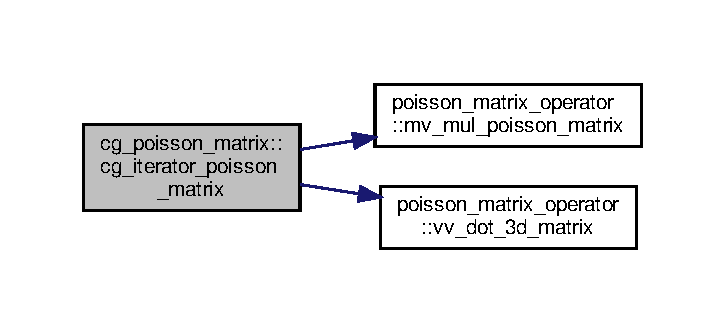
\includegraphics[width=348pt]{namespacecg__poisson__matrix_a558093032b9b1f54bf1bde7bfa847829_cgraph}
\end{center}
\end{figure}
\mbox{\Hypertarget{namespacecg__poisson__matrix_a4762a692c1b2dd5070d070e90a30e8cd}\label{namespacecg__poisson__matrix_a4762a692c1b2dd5070d070e90a30e8cd}} 
\index{cg\+\_\+poisson\+\_\+matrix@{cg\+\_\+poisson\+\_\+matrix}!cg\+\_\+solver\+\_\+poisson\+\_\+matrix@{cg\+\_\+solver\+\_\+poisson\+\_\+matrix}}
\index{cg\+\_\+solver\+\_\+poisson\+\_\+matrix@{cg\+\_\+solver\+\_\+poisson\+\_\+matrix}!cg\+\_\+poisson\+\_\+matrix@{cg\+\_\+poisson\+\_\+matrix}}
\subsubsection{\texorpdfstring{cg\+\_\+solver\+\_\+poisson\+\_\+matrix()}{cg\_solver\_poisson\_matrix()}}
{\footnotesize\ttfamily subroutine, public cg\+\_\+poisson\+\_\+matrix\+::cg\+\_\+solver\+\_\+poisson\+\_\+matrix (\begin{DoxyParamCaption}\item[{real(kind=8), dimension(0\+:,0\+:,0\+:), intent(inout)}]{sol,  }\item[{type(\hyperlink{structmatrix_1_1matrix__heptadiagonal}{matrix\+\_\+heptadiagonal}), intent(in)}]{a\+\_\+poisson,  }\item[{real(kind=8), dimension(0\+:,0\+:,0\+:), intent(in)}]{rhs,  }\item[{type(\hyperlink{structgeometry_1_1subdomain}{subdomain}), intent(in)}]{dm,  }\item[{integer(kind=4), intent(in)}]{maxiteration,  }\item[{real(kind=8), intent(in)}]{tolerance,  }\item[{logical, dimension(0\+:2), intent(in)}]{is\+\_\+aggregated }\end{DoxyParamCaption})}



Conjugate gradient solver with convergence criteria. 


\begin{DoxyParams}{Parameters}
{\em sol} & Result solution having a shape of 3D matrix \\
\hline
{\em a\+\_\+poisson} & Heptadiagonal poisson matrix \\
\hline
{\em rhs} & R\+HS vector having a shape of 3D matrix \\
\hline
{\em dm} & Subdomain \\
\hline
{\em maxiteration} & Maximum number of iterations \\
\hline
{\em tolerance} & Convergence criteria \\
\hline
{\em is\+\_\+aggregated} & Boolean whether domain is aggregated (.true.) or not (.false.) \\
\hline
\end{DoxyParams}
Here is the call graph for this function\+:
\nopagebreak
\begin{figure}[H]
\begin{center}
\leavevmode
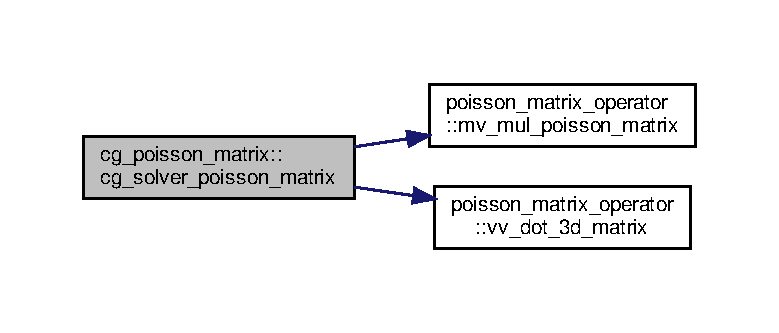
\includegraphics[width=350pt]{namespacecg__poisson__matrix_a4762a692c1b2dd5070d070e90a30e8cd_cgraph}
\end{center}
\end{figure}

\hypertarget{namespacegeometry}{}\section{geometry Module Reference}
\label{namespacegeometry}\index{geometry@{geometry}}


Module for building ubdomains from the physical global domain.  


\subsection*{Data Types}
\begin{DoxyCompactItemize}
\item 
type \hyperlink{structgeometry_1_1domain}{domain}
\begin{DoxyCompactList}\small\item\em Global domain information. \end{DoxyCompactList}\item 
type \hyperlink{structgeometry_1_1subdomain}{subdomain}
\begin{DoxyCompactList}\small\item\em Partitioned subdomain information. \end{DoxyCompactList}\end{DoxyCompactItemize}
\subsection*{Functions/\+Subroutines}
\begin{DoxyCompactItemize}
\item 
subroutine \hyperlink{namespacegeometry_a707b3bbf32a44b01c6a4f28e2be7d0fc}{geometry\+\_\+domain\+\_\+create} (gdm, nx, ny, nz, ox, oy, oz, lx, ly, lz, ax, ay, az, period)
\begin{DoxyCompactList}\small\item\em Prepare the global domain and grid information. \end{DoxyCompactList}\item 
subroutine \hyperlink{namespacegeometry_a46da96ff458eea5b671bec82e56dc6fb}{geometry\+\_\+domain\+\_\+destroy} (gdm)
\begin{DoxyCompactList}\small\item\em Free the variables of global domain. \end{DoxyCompactList}\item 
subroutine \hyperlink{namespacegeometry_ad0835bda792428d5f72a71aa6ebd1526}{geometry\+\_\+subdomain\+\_\+create} (sdm, gdm)
\begin{DoxyCompactList}\small\item\em Prepare the partitioned subdomain from global domain information. \end{DoxyCompactList}\item 
subroutine \hyperlink{namespacegeometry_ab546189e0ddda7aea0d8cd6e479ff8f1}{geometry\+\_\+subdomain\+\_\+destroy} (sdm)
\begin{DoxyCompactList}\small\item\em Free the variables of subdomain. \end{DoxyCompactList}\item 
subroutine \hyperlink{namespacegeometry_a559a7fbc4327cc9a54789163e414b6eb}{geometry\+\_\+subdomain\+\_\+ddt\+\_\+create} (sdm)
\begin{DoxyCompactList}\small\item\em Build derived datatypes for subdomain communication using ghostcells. \end{DoxyCompactList}\item 
subroutine \hyperlink{namespacegeometry_a29d3bd98ea090130609cf1dba291ceb4}{geometry\+\_\+subdomain\+\_\+ddt\+\_\+destroy} (sdm)
\begin{DoxyCompactList}\small\item\em Free derived datatypes for subdomain communication using ghostcells. \end{DoxyCompactList}\item 
subroutine \hyperlink{namespacegeometry_a28c9704c14f29b1f57c491246b206991}{geometry\+\_\+halocell\+\_\+update} (u, sdm)
\begin{DoxyCompactList}\small\item\em Update the values of boundary ghostcells through communication in all directions. \end{DoxyCompactList}\item 
subroutine \hyperlink{namespacegeometry_a13a9857b633f18041d764401c91d2918}{geometry\+\_\+halocell\+\_\+update\+\_\+selectively} (u, sdm, is\+\_\+serial)
\begin{DoxyCompactList}\small\item\em Update the values of boundary ghostcells through communication when the domain is not aggregated. \end{DoxyCompactList}\end{DoxyCompactItemize}


\subsection{Detailed Description}
Module for building ubdomains from the physical global domain. 

This module containes domain and grid information of global domain and subdomains. Derived Datatype for ghostcell communication between the subdomains is included. 

\subsection{Function/\+Subroutine Documentation}
\mbox{\Hypertarget{namespacegeometry_a707b3bbf32a44b01c6a4f28e2be7d0fc}\label{namespacegeometry_a707b3bbf32a44b01c6a4f28e2be7d0fc}} 
\index{geometry@{geometry}!geometry\+\_\+domain\+\_\+create@{geometry\+\_\+domain\+\_\+create}}
\index{geometry\+\_\+domain\+\_\+create@{geometry\+\_\+domain\+\_\+create}!geometry@{geometry}}
\subsubsection{\texorpdfstring{geometry\+\_\+domain\+\_\+create()}{geometry\_domain\_create()}}
{\footnotesize\ttfamily subroutine geometry\+::geometry\+\_\+domain\+\_\+create (\begin{DoxyParamCaption}\item[{type(\hyperlink{structgeometry_1_1domain}{domain}), intent(inout)}]{gdm,  }\item[{integer(kind=4), intent(in)}]{nx,  }\item[{integer(kind=4), intent(in)}]{ny,  }\item[{integer(kind=4), intent(in)}]{nz,  }\item[{real(kind=8), intent(in)}]{ox,  }\item[{real(kind=8), intent(in)}]{oy,  }\item[{real(kind=8), intent(in)}]{oz,  }\item[{real(kind=8), intent(in)}]{lx,  }\item[{real(kind=8), intent(in)}]{ly,  }\item[{real(kind=8), intent(in)}]{lz,  }\item[{real(kind=8), intent(in)}]{ax,  }\item[{real(kind=8), intent(in)}]{ay,  }\item[{real(kind=8), intent(in)}]{az,  }\item[{logical, dimension(0\+:2), intent(in)}]{period }\end{DoxyParamCaption})}



Prepare the global domain and grid information. 


\begin{DoxyParams}{Parameters}
{\em gdm} & Global domain \\
\hline
{\em nx} & Number of grid in x-\/direction \\
\hline
{\em ny} & Number of grid in y-\/direction \\
\hline
{\em nz} & Number of grid in z-\/direction \\
\hline
{\em ox} & Starting coordinate of global domain in x-\/direction \\
\hline
{\em oy} & Starting coordinate of global domain in y-\/direction \\
\hline
{\em oz} & Starting coordinate of global domain in z-\/direction \\
\hline
{\em lx} & Physical length of global domain in x-\/direction \\
\hline
{\em ly} & Physical length of global domain in y-\/direction \\
\hline
{\em lz} & Physical length of global domain in z-\/direction \\
\hline
{\em ax} & Mesh stretch ratio in x-\/direction \\
\hline
{\em ay} & Mesh stretch ratio in y-\/direction \\
\hline
{\em az} & Mesh stretch ratio in z-\/direction \\
\hline
{\em period} & Periodicity of global domain \\
\hline
\end{DoxyParams}
\mbox{\Hypertarget{namespacegeometry_a46da96ff458eea5b671bec82e56dc6fb}\label{namespacegeometry_a46da96ff458eea5b671bec82e56dc6fb}} 
\index{geometry@{geometry}!geometry\+\_\+domain\+\_\+destroy@{geometry\+\_\+domain\+\_\+destroy}}
\index{geometry\+\_\+domain\+\_\+destroy@{geometry\+\_\+domain\+\_\+destroy}!geometry@{geometry}}
\subsubsection{\texorpdfstring{geometry\+\_\+domain\+\_\+destroy()}{geometry\_domain\_destroy()}}
{\footnotesize\ttfamily subroutine geometry\+::geometry\+\_\+domain\+\_\+destroy (\begin{DoxyParamCaption}\item[{type(\hyperlink{structgeometry_1_1domain}{domain}), intent(inout)}]{gdm }\end{DoxyParamCaption})}



Free the variables of global domain. 


\begin{DoxyParams}{Parameters}
{\em gdm} & Global domain \\
\hline
\end{DoxyParams}
\mbox{\Hypertarget{namespacegeometry_a28c9704c14f29b1f57c491246b206991}\label{namespacegeometry_a28c9704c14f29b1f57c491246b206991}} 
\index{geometry@{geometry}!geometry\+\_\+halocell\+\_\+update@{geometry\+\_\+halocell\+\_\+update}}
\index{geometry\+\_\+halocell\+\_\+update@{geometry\+\_\+halocell\+\_\+update}!geometry@{geometry}}
\subsubsection{\texorpdfstring{geometry\+\_\+halocell\+\_\+update()}{geometry\_halocell\_update()}}
{\footnotesize\ttfamily subroutine geometry\+::geometry\+\_\+halocell\+\_\+update (\begin{DoxyParamCaption}\item[{real(kind=8), dimension(0\+:,0\+:,0\+:), intent(inout)}]{u,  }\item[{type(\hyperlink{structgeometry_1_1subdomain}{subdomain}), intent(in)}]{sdm }\end{DoxyParamCaption})}



Update the values of boundary ghostcells through communication in all directions. 


\begin{DoxyParams}{Parameters}
{\em u} & Grid variable to be updated \\
\hline
{\em sdm} & Subdomain \\
\hline
\end{DoxyParams}
\mbox{\Hypertarget{namespacegeometry_a13a9857b633f18041d764401c91d2918}\label{namespacegeometry_a13a9857b633f18041d764401c91d2918}} 
\index{geometry@{geometry}!geometry\+\_\+halocell\+\_\+update\+\_\+selectively@{geometry\+\_\+halocell\+\_\+update\+\_\+selectively}}
\index{geometry\+\_\+halocell\+\_\+update\+\_\+selectively@{geometry\+\_\+halocell\+\_\+update\+\_\+selectively}!geometry@{geometry}}
\subsubsection{\texorpdfstring{geometry\+\_\+halocell\+\_\+update\+\_\+selectively()}{geometry\_halocell\_update\_selectively()}}
{\footnotesize\ttfamily subroutine geometry\+::geometry\+\_\+halocell\+\_\+update\+\_\+selectively (\begin{DoxyParamCaption}\item[{real(kind=8), dimension(0\+:,0\+:,0\+:), intent(inout)}]{u,  }\item[{type(\hyperlink{structgeometry_1_1subdomain}{subdomain}), intent(in)}]{sdm,  }\item[{logical, dimension(0\+:2), intent(in)}]{is\+\_\+serial }\end{DoxyParamCaption})}



Update the values of boundary ghostcells through communication when the domain is not aggregated. 


\begin{DoxyParams}{Parameters}
{\em u} & Grid variable to be updated \\
\hline
{\em sdm} & Subdomain \\
\hline
{\em is\+\_\+serial} & Boolean whether the subdomain is aggregated(.true.) or not(.false.) \\
\hline
\end{DoxyParams}
\mbox{\Hypertarget{namespacegeometry_ad0835bda792428d5f72a71aa6ebd1526}\label{namespacegeometry_ad0835bda792428d5f72a71aa6ebd1526}} 
\index{geometry@{geometry}!geometry\+\_\+subdomain\+\_\+create@{geometry\+\_\+subdomain\+\_\+create}}
\index{geometry\+\_\+subdomain\+\_\+create@{geometry\+\_\+subdomain\+\_\+create}!geometry@{geometry}}
\subsubsection{\texorpdfstring{geometry\+\_\+subdomain\+\_\+create()}{geometry\_subdomain\_create()}}
{\footnotesize\ttfamily subroutine geometry\+::geometry\+\_\+subdomain\+\_\+create (\begin{DoxyParamCaption}\item[{type(\hyperlink{structgeometry_1_1subdomain}{subdomain}), intent(inout)}]{sdm,  }\item[{type(\hyperlink{structgeometry_1_1domain}{domain}), intent(in)}]{gdm }\end{DoxyParamCaption})}



Prepare the partitioned subdomain from global domain information. 


\begin{DoxyParams}{Parameters}
{\em gdm} & Global domain \\
\hline
{\em sdm} & Partitioned subdomain \\
\hline
\end{DoxyParams}
Here is the call graph for this function\+:
\nopagebreak
\begin{figure}[H]
\begin{center}
\leavevmode
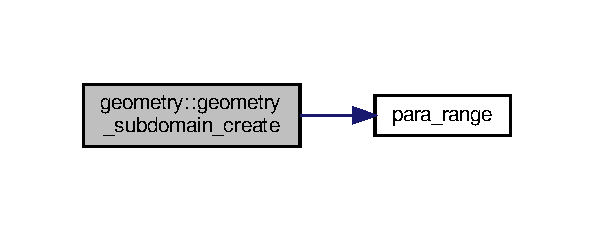
\includegraphics[width=285pt]{namespacegeometry_ad0835bda792428d5f72a71aa6ebd1526_cgraph}
\end{center}
\end{figure}
\mbox{\Hypertarget{namespacegeometry_a559a7fbc4327cc9a54789163e414b6eb}\label{namespacegeometry_a559a7fbc4327cc9a54789163e414b6eb}} 
\index{geometry@{geometry}!geometry\+\_\+subdomain\+\_\+ddt\+\_\+create@{geometry\+\_\+subdomain\+\_\+ddt\+\_\+create}}
\index{geometry\+\_\+subdomain\+\_\+ddt\+\_\+create@{geometry\+\_\+subdomain\+\_\+ddt\+\_\+create}!geometry@{geometry}}
\subsubsection{\texorpdfstring{geometry\+\_\+subdomain\+\_\+ddt\+\_\+create()}{geometry\_subdomain\_ddt\_create()}}
{\footnotesize\ttfamily subroutine geometry\+::geometry\+\_\+subdomain\+\_\+ddt\+\_\+create (\begin{DoxyParamCaption}\item[{type(\hyperlink{structgeometry_1_1subdomain}{subdomain}), intent(inout)}]{sdm }\end{DoxyParamCaption})}



Build derived datatypes for subdomain communication using ghostcells. 


\begin{DoxyParams}{Parameters}
{\em sdm} & Subdomain \\
\hline
\end{DoxyParams}
\mbox{\Hypertarget{namespacegeometry_a29d3bd98ea090130609cf1dba291ceb4}\label{namespacegeometry_a29d3bd98ea090130609cf1dba291ceb4}} 
\index{geometry@{geometry}!geometry\+\_\+subdomain\+\_\+ddt\+\_\+destroy@{geometry\+\_\+subdomain\+\_\+ddt\+\_\+destroy}}
\index{geometry\+\_\+subdomain\+\_\+ddt\+\_\+destroy@{geometry\+\_\+subdomain\+\_\+ddt\+\_\+destroy}!geometry@{geometry}}
\subsubsection{\texorpdfstring{geometry\+\_\+subdomain\+\_\+ddt\+\_\+destroy()}{geometry\_subdomain\_ddt\_destroy()}}
{\footnotesize\ttfamily subroutine geometry\+::geometry\+\_\+subdomain\+\_\+ddt\+\_\+destroy (\begin{DoxyParamCaption}\item[{type(\hyperlink{structgeometry_1_1subdomain}{subdomain}), intent(inout)}]{sdm }\end{DoxyParamCaption})}



Free derived datatypes for subdomain communication using ghostcells. 


\begin{DoxyParams}{Parameters}
{\em sdm} & subdomain \\
\hline
\end{DoxyParams}
\mbox{\Hypertarget{namespacegeometry_ab546189e0ddda7aea0d8cd6e479ff8f1}\label{namespacegeometry_ab546189e0ddda7aea0d8cd6e479ff8f1}} 
\index{geometry@{geometry}!geometry\+\_\+subdomain\+\_\+destroy@{geometry\+\_\+subdomain\+\_\+destroy}}
\index{geometry\+\_\+subdomain\+\_\+destroy@{geometry\+\_\+subdomain\+\_\+destroy}!geometry@{geometry}}
\subsubsection{\texorpdfstring{geometry\+\_\+subdomain\+\_\+destroy()}{geometry\_subdomain\_destroy()}}
{\footnotesize\ttfamily subroutine geometry\+::geometry\+\_\+subdomain\+\_\+destroy (\begin{DoxyParamCaption}\item[{type(\hyperlink{structgeometry_1_1subdomain}{subdomain}), intent(inout)}]{sdm }\end{DoxyParamCaption})}



Free the variables of subdomain. 


\begin{DoxyParams}{Parameters}
{\em sdm} & Subdomain \\
\hline
\end{DoxyParams}

\hypertarget{namespacematrix}{}\section{matrix Module Reference}
\label{namespacematrix}\index{matrix@{matrix}}


Module for matrix type for finite difference method with 7-\/stencil points.  


\subsection*{Data Types}
\begin{DoxyCompactItemize}
\item 
type \hyperlink{structmatrix_1_1matrix__heptadiagonal}{matrix\+\_\+heptadiagonal}
\begin{DoxyCompactList}\small\item\em Heptadiagonam matrix for finite difference method with 7-\/stencil points. \end{DoxyCompactList}\end{DoxyCompactItemize}
\subsection*{Functions/\+Subroutines}
\begin{DoxyCompactItemize}
\item 
subroutine \hyperlink{namespacematrix_af96fcc5a5c79a720967847d6569ce479}{matrix\+\_\+heptadiagonal\+\_\+create} (a\+\_\+poisson, sdm)
\begin{DoxyCompactList}\small\item\em Create the heptadiagonal matrix for finite difference method with 7-\/stencil points. \end{DoxyCompactList}\item 
subroutine \hyperlink{namespacematrix_a1c201958a669deaddeb6aa76251b394f}{matrix\+\_\+heptadiagonal\+\_\+destroy} (a\+\_\+poisson)
\begin{DoxyCompactList}\small\item\em Destroy the heptadiagonal matrix for finite difference method with 7-\/stencil points. \end{DoxyCompactList}\end{DoxyCompactItemize}


\subsection{Detailed Description}
Module for matrix type for finite difference method with 7-\/stencil points. 

The module containes the matrix type, its creator and destroyer. 

\subsection{Function/\+Subroutine Documentation}
\mbox{\Hypertarget{namespacematrix_af96fcc5a5c79a720967847d6569ce479}\label{namespacematrix_af96fcc5a5c79a720967847d6569ce479}} 
\index{matrix@{matrix}!matrix\+\_\+heptadiagonal\+\_\+create@{matrix\+\_\+heptadiagonal\+\_\+create}}
\index{matrix\+\_\+heptadiagonal\+\_\+create@{matrix\+\_\+heptadiagonal\+\_\+create}!matrix@{matrix}}
\subsubsection{\texorpdfstring{matrix\+\_\+heptadiagonal\+\_\+create()}{matrix\_heptadiagonal\_create()}}
{\footnotesize\ttfamily subroutine matrix\+::matrix\+\_\+heptadiagonal\+\_\+create (\begin{DoxyParamCaption}\item[{type(\hyperlink{structmatrix_1_1matrix__heptadiagonal}{matrix\+\_\+heptadiagonal}), intent(inout)}]{a\+\_\+poisson,  }\item[{type(\hyperlink{structgeometry_1_1subdomain}{subdomain}), intent(in)}]{sdm }\end{DoxyParamCaption})}



Create the heptadiagonal matrix for finite difference method with 7-\/stencil points. 


\begin{DoxyParams}{Parameters}
{\em a\+\_\+poisson} & Matrix of \hyperlink{structmatrix_1_1matrix__heptadiagonal}{matrix\+\_\+heptadiagonal} type \\
\hline
{\em sdm} & Subdomain \\
\hline
\end{DoxyParams}
Here is the caller graph for this function\+:
\nopagebreak
\begin{figure}[H]
\begin{center}
\leavevmode
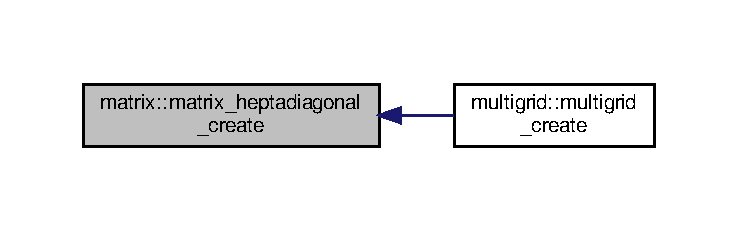
\includegraphics[width=350pt]{namespacematrix_af96fcc5a5c79a720967847d6569ce479_icgraph}
\end{center}
\end{figure}
\mbox{\Hypertarget{namespacematrix_a1c201958a669deaddeb6aa76251b394f}\label{namespacematrix_a1c201958a669deaddeb6aa76251b394f}} 
\index{matrix@{matrix}!matrix\+\_\+heptadiagonal\+\_\+destroy@{matrix\+\_\+heptadiagonal\+\_\+destroy}}
\index{matrix\+\_\+heptadiagonal\+\_\+destroy@{matrix\+\_\+heptadiagonal\+\_\+destroy}!matrix@{matrix}}
\subsubsection{\texorpdfstring{matrix\+\_\+heptadiagonal\+\_\+destroy()}{matrix\_heptadiagonal\_destroy()}}
{\footnotesize\ttfamily subroutine matrix\+::matrix\+\_\+heptadiagonal\+\_\+destroy (\begin{DoxyParamCaption}\item[{type(\hyperlink{structmatrix_1_1matrix__heptadiagonal}{matrix\+\_\+heptadiagonal}), intent(inout)}]{a\+\_\+poisson }\end{DoxyParamCaption})}



Destroy the heptadiagonal matrix for finite difference method with 7-\/stencil points. 


\begin{DoxyParams}{Parameters}
{\em a\+\_\+poisson} & Matrix of \hyperlink{structmatrix_1_1matrix__heptadiagonal}{matrix\+\_\+heptadiagonal} type \\
\hline
\end{DoxyParams}
Here is the caller graph for this function\+:
\nopagebreak
\begin{figure}[H]
\begin{center}
\leavevmode
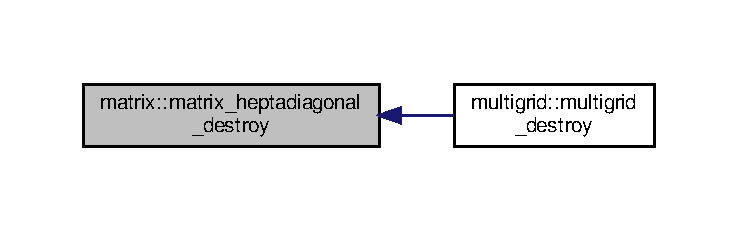
\includegraphics[width=350pt]{namespacematrix_a1c201958a669deaddeb6aa76251b394f_icgraph}
\end{center}
\end{figure}

\hypertarget{namespacempi__topology}{}\section{mpi\+\_\+topology Module Reference}
\label{namespacempi__topology}\index{mpi\+\_\+topology@{mpi\+\_\+topology}}


Module for creating the cartesian topology of the M\+PI processes and subcommunicators.  


\subsection*{Data Types}
\begin{DoxyCompactItemize}
\item 
type \hyperlink{structmpi__topology_1_1cart__comm__1d}{cart\+\_\+comm\+\_\+1d}
\begin{DoxyCompactList}\small\item\em Type variable for the information of 1D communicator. \end{DoxyCompactList}\end{DoxyCompactItemize}
\subsection*{Functions/\+Subroutines}
\begin{DoxyCompactItemize}
\item 
\mbox{\Hypertarget{namespacempi__topology_ae299dc83f2e6767402df3dfacfad4e44}\label{namespacempi__topology_ae299dc83f2e6767402df3dfacfad4e44}} 
subroutine, public \hyperlink{namespacempi__topology_ae299dc83f2e6767402df3dfacfad4e44}{mpi\+\_\+topology\+\_\+create} ()
\begin{DoxyCompactList}\small\item\em Create the cartesian topology for the M\+PI processes and subcommunicators. \end{DoxyCompactList}\item 
\mbox{\Hypertarget{namespacempi__topology_a27582d0f86406910fa43ad925ac38801}\label{namespacempi__topology_a27582d0f86406910fa43ad925ac38801}} 
subroutine, public \hyperlink{namespacempi__topology_a27582d0f86406910fa43ad925ac38801}{mpi\+\_\+topology\+\_\+destroy} ()
\begin{DoxyCompactList}\small\item\em Destroy the communicator for cartesian topology. \end{DoxyCompactList}\end{DoxyCompactItemize}
\subsection*{Variables}
\begin{DoxyCompactItemize}
\item 
\mbox{\Hypertarget{namespacempi__topology_a893b6fb583833278f1fd992cd4d4cbf8}\label{namespacempi__topology_a893b6fb583833278f1fd992cd4d4cbf8}} 
integer(kind=4), public \hyperlink{namespacempi__topology_a893b6fb583833278f1fd992cd4d4cbf8}{mpi\+\_\+world\+\_\+cart}
\begin{DoxyCompactList}\small\item\em Communicator for cartesian topology. \end{DoxyCompactList}\item 
\mbox{\Hypertarget{namespacempi__topology_af16caa219178ffc6fb90822629db8a49}\label{namespacempi__topology_af16caa219178ffc6fb90822629db8a49}} 
integer(kind=4), public {\bfseries nprocs}
\item 
\mbox{\Hypertarget{namespacempi__topology_a27f9bdf05c9c90f0c087aeb26b99a4f3}\label{namespacempi__topology_a27f9bdf05c9c90f0c087aeb26b99a4f3}} 
integer(kind=4), public \hyperlink{namespacempi__topology_a27f9bdf05c9c90f0c087aeb26b99a4f3}{myrank}
\begin{DoxyCompactList}\small\item\em Number of processes and rank ID in M\+P\+I\+\_\+\+C\+O\+M\+M\+\_\+\+W\+O\+R\+LD. \end{DoxyCompactList}\item 
\mbox{\Hypertarget{namespacempi__topology_a8f8932a2511cfd89285a6f2eb906d098}\label{namespacempi__topology_a8f8932a2511cfd89285a6f2eb906d098}} 
integer(kind=4), dimension(0\+:2), public \hyperlink{namespacempi__topology_a8f8932a2511cfd89285a6f2eb906d098}{np\+\_\+dim}
\begin{DoxyCompactList}\small\item\em Number of M\+PI processes in 3D topology. \end{DoxyCompactList}\item 
\mbox{\Hypertarget{namespacempi__topology_ac24cb383bdfbdf566165cf78b03677aa}\label{namespacempi__topology_ac24cb383bdfbdf566165cf78b03677aa}} 
logical, dimension(0\+:2), public \hyperlink{namespacempi__topology_ac24cb383bdfbdf566165cf78b03677aa}{period}
\begin{DoxyCompactList}\small\item\em Periodicity in each direction. \end{DoxyCompactList}\item 
\mbox{\Hypertarget{namespacempi__topology_a67d857c7a471473332bbfcac7682943c}\label{namespacempi__topology_a67d857c7a471473332bbfcac7682943c}} 
type(\hyperlink{structmpi__topology_1_1cart__comm__1d}{cart\+\_\+comm\+\_\+1d}), target, public \hyperlink{namespacempi__topology_a67d857c7a471473332bbfcac7682943c}{comm\+\_\+1d\+\_\+x}
\begin{DoxyCompactList}\small\item\em Subcommunicator information in x-\/direction. \end{DoxyCompactList}\item 
\mbox{\Hypertarget{namespacempi__topology_a4f667ff8f1bbfd8075bd7629cba14c2d}\label{namespacempi__topology_a4f667ff8f1bbfd8075bd7629cba14c2d}} 
type(\hyperlink{structmpi__topology_1_1cart__comm__1d}{cart\+\_\+comm\+\_\+1d}), target, public \hyperlink{namespacempi__topology_a4f667ff8f1bbfd8075bd7629cba14c2d}{comm\+\_\+1d\+\_\+y}
\begin{DoxyCompactList}\small\item\em Subcommunicator information in y-\/direction. \end{DoxyCompactList}\item 
\mbox{\Hypertarget{namespacempi__topology_a9d5db9f9841b438a50d1809aaf8f0efc}\label{namespacempi__topology_a9d5db9f9841b438a50d1809aaf8f0efc}} 
type(\hyperlink{structmpi__topology_1_1cart__comm__1d}{cart\+\_\+comm\+\_\+1d}), target, public \hyperlink{namespacempi__topology_a9d5db9f9841b438a50d1809aaf8f0efc}{comm\+\_\+1d\+\_\+z}
\begin{DoxyCompactList}\small\item\em Subcommunicator information in z-\/direction. \end{DoxyCompactList}\end{DoxyCompactItemize}


\subsection{Detailed Description}
Module for creating the cartesian topology of the M\+PI processes and subcommunicators. 

This module has three subcommunicators in each-\/direction and related subroutines. 
\hypertarget{namespacemultigrid}{}\section{multigrid Module Reference}
\label{namespacemultigrid}\index{multigrid@{multigrid}}


Module for solving Poisson equation with V-\/cycle multigrid(\+M\+G) method.  C\+GS, C\+GA and C\+G\+P\+SA are supported in this module. C\+GS \+: Coarse grid solver without grid aggregation. C\+GA \+: Coarse grid aggregation in a target level. All grid variables are aggregated into a singel core. C\+G\+P\+SA \+: Coarse grid partial semi-\/aggregation in multiple levels.!$>$  


\subsection*{Functions/\+Subroutines}
\begin{DoxyCompactItemize}
\item 
subroutine, public \hyperlink{namespacemultigrid_ac8deb32ba5698e37f75c369dc063b277}{multigrid\+\_\+create} (sdm, nlevel, ncycle, aggr\+\_\+method, single\+\_\+aggr\+\_\+level, adaptive\+\_\+aggr\+\_\+level)
\begin{DoxyCompactList}\small\item\em Create MG subdomains and Poisson matrix  MG subdomain depends on aggregation type. Different subroutines are called according to aggregation type. \end{DoxyCompactList}\item 
\mbox{\Hypertarget{namespacemultigrid_a07ed47be36b2e0df9d71ec58151b642b}\label{namespacemultigrid_a07ed47be36b2e0df9d71ec58151b642b}} 
subroutine, public \hyperlink{namespacemultigrid_a07ed47be36b2e0df9d71ec58151b642b}{multigrid\+\_\+destroy}
\begin{DoxyCompactList}\small\item\em Destroy all variables in all MG subdomains. \end{DoxyCompactList}\item 
subroutine \hyperlink{namespacemultigrid_a839d1e13e2d0bac4959deec5669d4171}{multigrid\+\_\+prolongation\+\_\+linear\+\_\+on\+\_\+nonuniform\+\_\+grid} (val\+\_\+f, val\+\_\+c, dm\+\_\+f, dm\+\_\+c, level)
\begin{DoxyCompactList}\small\item\em Prolongation subroutine for C\+GS, C\+GA, and C\+G\+P\+SA  This subroutine is commonly used by using stride\+\_\+f and offest\+\_\+f variables Constant profile in assumed in finer level. \end{DoxyCompactList}\item 
subroutine \hyperlink{namespacemultigrid_ad1ba34848f786afdf0e91afb3d3be819}{multigrid\+\_\+residual} (rsd, a\+\_\+poisson, x, rhs, dm, is\+\_\+aggregated)
\begin{DoxyCompactList}\small\item\em Residual calculation. rsd = rhs -\/ a\+\_\+poisson $\ast$ x. \end{DoxyCompactList}\item 
subroutine, public \hyperlink{namespacemultigrid_a7d60c9d01777350a79ff7bd975a90121}{multigrid\+\_\+solve\+\_\+vcycle} (sol, rsd, a\+\_\+poisson, rhs, sdm, maxiteration, tolerance, omega\+\_\+sor)
\begin{DoxyCompactList}\small\item\em V-\/\+Cycle MG solver\+: call subroutines according to aggregation type. \end{DoxyCompactList}\item 
subroutine \hyperlink{namespacemultigrid_aa8278baf0276649fe656c1b8f7dba30a}{multigrid\+\_\+cgs\+\_\+vcycle\+\_\+solver} (sol, rsd, a\+\_\+poisson, rhs, sdm, maxiteration, tolerance, omega\+\_\+sor)
\begin{DoxyCompactList}\small\item\em V-\/\+Cycle MG solver with C\+GS. \end{DoxyCompactList}\item 
subroutine \hyperlink{namespacemultigrid_a4295ca0af002ede1dee98750922f1f60}{multigrid\+\_\+cga\+\_\+vcycle\+\_\+solver} (sol, rsd, a\+\_\+poisson, rhs, sdm, maxiteration, tolerance, omega\+\_\+sor)
\begin{DoxyCompactList}\small\item\em V-\/\+Cycle MG solver with C\+GA  M\+P\+I\+\_\+\+Gather/\+M\+P\+I\+\_\+\+Scatterv with derived datatypes are used for aggregation. \end{DoxyCompactList}\item 
subroutine \hyperlink{namespacemultigrid_ae89565627880985244634750502edab5}{multigrid\+\_\+cgpsa\+\_\+vcycle\+\_\+solver} (sol, rsd, a\+\_\+poisson, rhs, sdm, maxiteration, tolerance, omega\+\_\+sor)
\begin{DoxyCompactList}\small\item\em V-\/\+Cycle MG solver with C\+G\+P\+SA  M\+P\+I\+\_\+\+Gather/\+M\+P\+I\+\_\+\+Scatterv with derived datatypes are used for aggregation. \end{DoxyCompactList}\end{DoxyCompactItemize}
\textbf{ }\par
\begin{DoxyCompactItemize}
\item 
subroutine \hyperlink{namespacemultigrid_acb52ce247bf637e69274d8da44d1f159}{multigrid\+\_\+subdomain\+\_\+create\+\_\+cgs} (sdm)
\begin{DoxyCompactList}\small\item\em Create MG subdomains for C\+GS  Define MG domain and assign grid dimensions such as mesh size, grid spacing and grid coordinates in each MG levels. \end{DoxyCompactList}\end{DoxyCompactItemize}

\textbf{ }\par
\begin{DoxyCompactItemize}
\item 
subroutine \hyperlink{namespacemultigrid_ae33e2e076cc087e7d149a3150c1ca1af}{multigrid\+\_\+subdomain\+\_\+create\+\_\+cga} (sdm)
\begin{DoxyCompactList}\small\item\em Create MG subdomains for C\+GA  Define MG domain and assign grid dimensions such as mesh size, grid spacing and grid coordinates in each MG levels. \end{DoxyCompactList}\end{DoxyCompactItemize}

\textbf{ }\par
\begin{DoxyCompactItemize}
\item 
subroutine \hyperlink{namespacemultigrid_aa2eb7c900fb5875f844c04c27c552373}{multigrid\+\_\+subdomain\+\_\+create\+\_\+cgpsa} (sdm)
\begin{DoxyCompactList}\small\item\em Create MG subdomains for C\+G\+P\+SA  Define MG domain and assign grid dimensions such as mesh size, grid spacing and grid coordinates in each MG levels. \end{DoxyCompactList}\end{DoxyCompactItemize}



\subsection{Detailed Description}
Module for solving Poisson equation with V-\/cycle multigrid(\+M\+G) method.  C\+GS, C\+GA and C\+G\+P\+SA are supported in this module. C\+GS \+: Coarse grid solver without grid aggregation. C\+GA \+: Coarse grid aggregation in a target level. All grid variables are aggregated into a singel core. C\+G\+P\+SA \+: Coarse grid partial semi-\/aggregation in multiple levels.!$>$ 

\subsection{Function/\+Subroutine Documentation}
\mbox{\Hypertarget{namespacemultigrid_a4295ca0af002ede1dee98750922f1f60}\label{namespacemultigrid_a4295ca0af002ede1dee98750922f1f60}} 
\index{multigrid@{multigrid}!multigrid\+\_\+cga\+\_\+vcycle\+\_\+solver@{multigrid\+\_\+cga\+\_\+vcycle\+\_\+solver}}
\index{multigrid\+\_\+cga\+\_\+vcycle\+\_\+solver@{multigrid\+\_\+cga\+\_\+vcycle\+\_\+solver}!multigrid@{multigrid}}
\subsubsection{\texorpdfstring{multigrid\+\_\+cga\+\_\+vcycle\+\_\+solver()}{multigrid\_cga\_vcycle\_solver()}}
{\footnotesize\ttfamily subroutine multigrid\+::multigrid\+\_\+cga\+\_\+vcycle\+\_\+solver (\begin{DoxyParamCaption}\item[{real(kind=8), dimension(0\+:,0\+:,0\+:), intent(inout)}]{sol,  }\item[{real(kind=8), dimension(0\+:,0\+:,0\+:), intent(inout)}]{rsd,  }\item[{type(\hyperlink{structmatrix_1_1matrix__heptadiagonal}{matrix\+\_\+heptadiagonal}), intent(in)}]{a\+\_\+poisson,  }\item[{real(kind=8), dimension(0\+:,0\+:,0\+:), intent(in)}]{rhs,  }\item[{type(\hyperlink{structgeometry_1_1subdomain}{subdomain}), intent(in)}]{sdm,  }\item[{integer(kind=4), intent(in)}]{maxiteration,  }\item[{real(kind=8), intent(in)}]{tolerance,  }\item[{real(kind=8), intent(in)}]{omega\+\_\+sor }\end{DoxyParamCaption})}



V-\/\+Cycle MG solver with C\+GA  M\+P\+I\+\_\+\+Gather/\+M\+P\+I\+\_\+\+Scatterv with derived datatypes are used for aggregation. 


\begin{DoxyParams}{Parameters}
{\em sol} & Result solution having a shape of 3D matrix \\
\hline
{\em rsd} & Residual \\
\hline
{\em a\+\_\+poisson} & Heptadiagonal poisson matrix \\
\hline
{\em rhs} & R\+HS vector having a shape of 3D matrix \\
\hline
{\em sdm} & Subdomain \\
\hline
{\em maxiteration} & Maximum number of iterations \\
\hline
{\em tolerance} & Convergence criteria \\
\hline
{\em omega\+\_\+sor} & Relexation factor \\
\hline
\end{DoxyParams}
Here is the call graph for this function\+:
\nopagebreak
\begin{figure}[H]
\begin{center}
\leavevmode
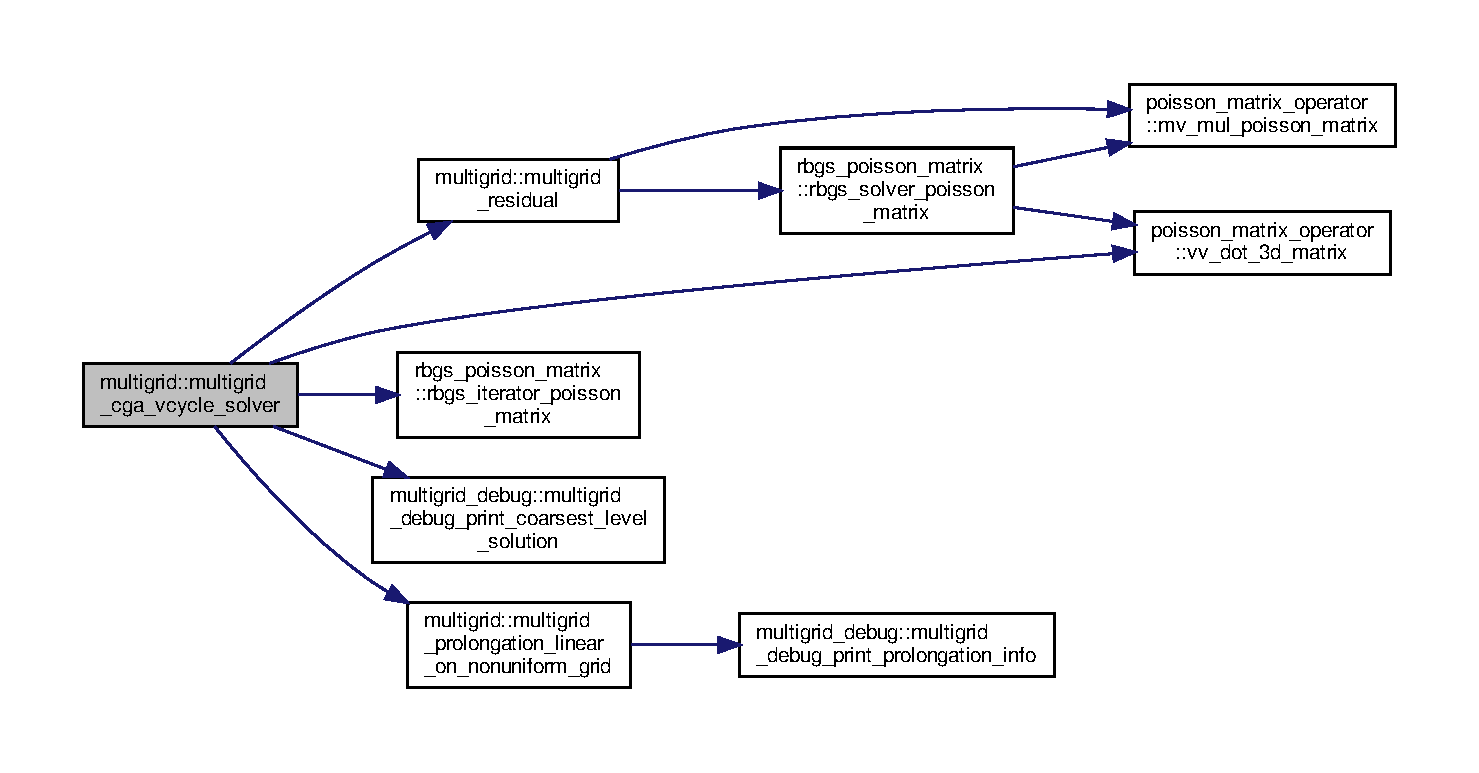
\includegraphics[width=350pt]{namespacemultigrid_a4295ca0af002ede1dee98750922f1f60_cgraph}
\end{center}
\end{figure}
Here is the caller graph for this function\+:
\nopagebreak
\begin{figure}[H]
\begin{center}
\leavevmode
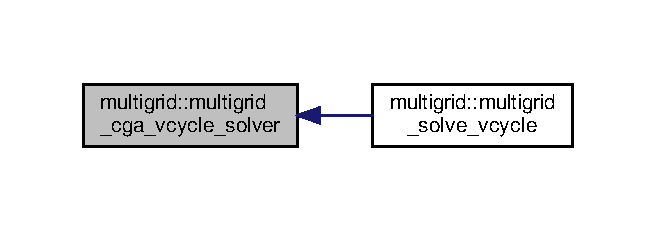
\includegraphics[width=315pt]{namespacemultigrid_a4295ca0af002ede1dee98750922f1f60_icgraph}
\end{center}
\end{figure}
\mbox{\Hypertarget{namespacemultigrid_ae89565627880985244634750502edab5}\label{namespacemultigrid_ae89565627880985244634750502edab5}} 
\index{multigrid@{multigrid}!multigrid\+\_\+cgpsa\+\_\+vcycle\+\_\+solver@{multigrid\+\_\+cgpsa\+\_\+vcycle\+\_\+solver}}
\index{multigrid\+\_\+cgpsa\+\_\+vcycle\+\_\+solver@{multigrid\+\_\+cgpsa\+\_\+vcycle\+\_\+solver}!multigrid@{multigrid}}
\subsubsection{\texorpdfstring{multigrid\+\_\+cgpsa\+\_\+vcycle\+\_\+solver()}{multigrid\_cgpsa\_vcycle\_solver()}}
{\footnotesize\ttfamily subroutine multigrid\+::multigrid\+\_\+cgpsa\+\_\+vcycle\+\_\+solver (\begin{DoxyParamCaption}\item[{real(kind=8), dimension(0\+:,0\+:,0\+:), intent(inout)}]{sol,  }\item[{real(kind=8), dimension(0\+:,0\+:,0\+:), intent(inout)}]{rsd,  }\item[{type(\hyperlink{structmatrix_1_1matrix__heptadiagonal}{matrix\+\_\+heptadiagonal}), intent(in)}]{a\+\_\+poisson,  }\item[{real(kind=8), dimension(0\+:,0\+:,0\+:), intent(in)}]{rhs,  }\item[{type(\hyperlink{structgeometry_1_1subdomain}{subdomain}), intent(in)}]{sdm,  }\item[{integer(kind=4), intent(in)}]{maxiteration,  }\item[{real(kind=8), intent(in)}]{tolerance,  }\item[{real(kind=8), intent(in)}]{omega\+\_\+sor }\end{DoxyParamCaption})}



V-\/\+Cycle MG solver with C\+G\+P\+SA  M\+P\+I\+\_\+\+Gather/\+M\+P\+I\+\_\+\+Scatterv with derived datatypes are used for aggregation. 


\begin{DoxyParams}{Parameters}
{\em sol} & Result solution having a shape of 3D matrix \\
\hline
{\em rsd} & Residual \\
\hline
{\em a\+\_\+poisson} & Heptadiagonal poisson matrix \\
\hline
{\em rhs} & R\+HS vector having a shape of 3D matrix \\
\hline
{\em sdm} & Subdomain \\
\hline
{\em maxiteration} & Maximum number of iterations \\
\hline
{\em tolerance} & Convergence criteria \\
\hline
{\em omega\+\_\+sor} & Relexation factor \\
\hline
\end{DoxyParams}
Here is the call graph for this function\+:
\nopagebreak
\begin{figure}[H]
\begin{center}
\leavevmode
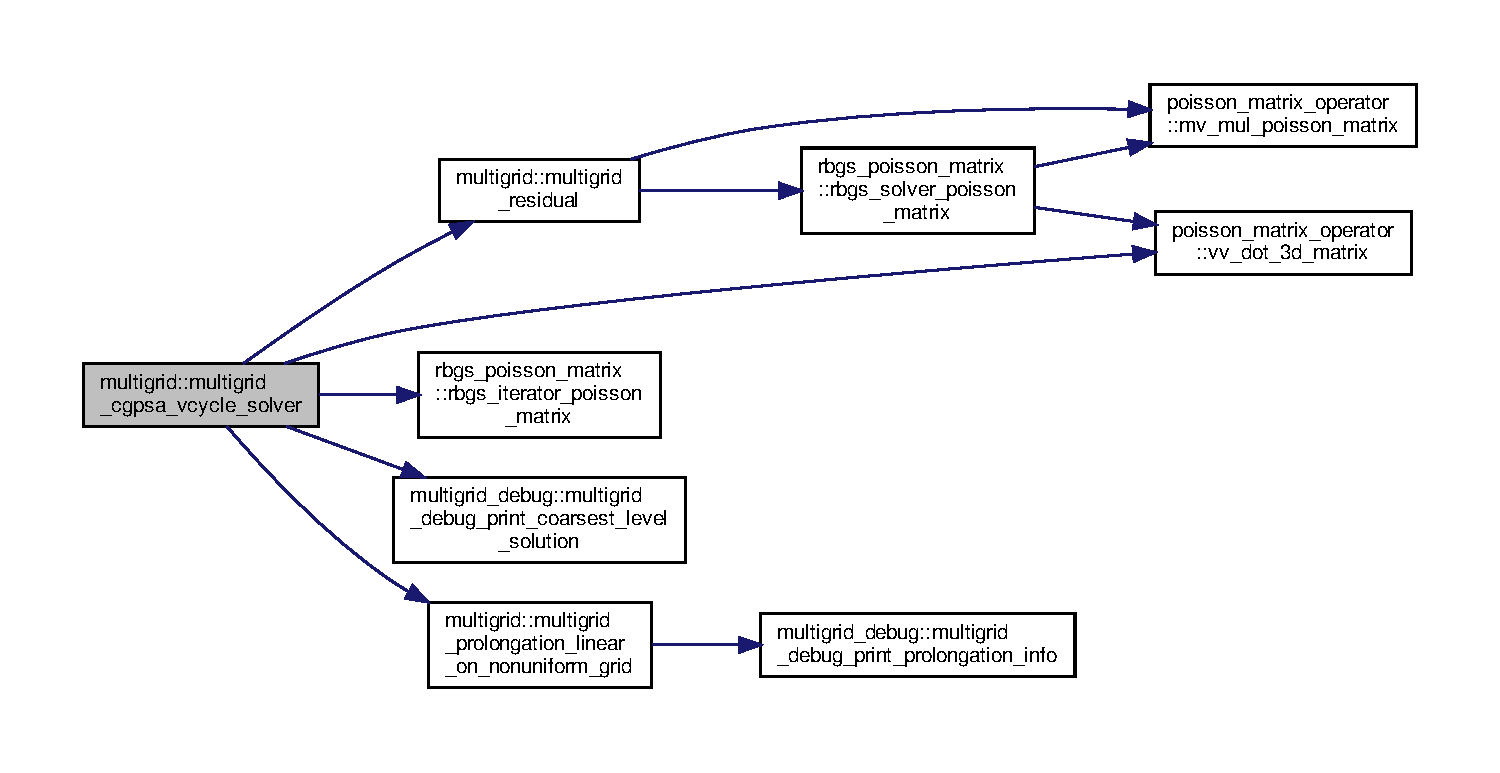
\includegraphics[width=350pt]{namespacemultigrid_ae89565627880985244634750502edab5_cgraph}
\end{center}
\end{figure}
Here is the caller graph for this function\+:
\nopagebreak
\begin{figure}[H]
\begin{center}
\leavevmode
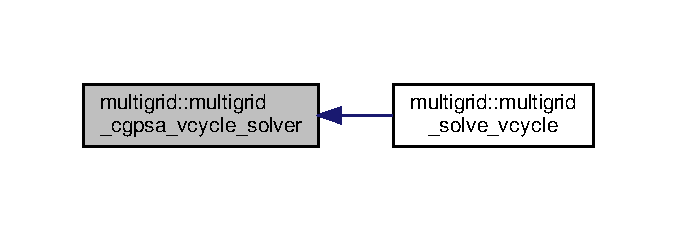
\includegraphics[width=325pt]{namespacemultigrid_ae89565627880985244634750502edab5_icgraph}
\end{center}
\end{figure}
\mbox{\Hypertarget{namespacemultigrid_aa8278baf0276649fe656c1b8f7dba30a}\label{namespacemultigrid_aa8278baf0276649fe656c1b8f7dba30a}} 
\index{multigrid@{multigrid}!multigrid\+\_\+cgs\+\_\+vcycle\+\_\+solver@{multigrid\+\_\+cgs\+\_\+vcycle\+\_\+solver}}
\index{multigrid\+\_\+cgs\+\_\+vcycle\+\_\+solver@{multigrid\+\_\+cgs\+\_\+vcycle\+\_\+solver}!multigrid@{multigrid}}
\subsubsection{\texorpdfstring{multigrid\+\_\+cgs\+\_\+vcycle\+\_\+solver()}{multigrid\_cgs\_vcycle\_solver()}}
{\footnotesize\ttfamily subroutine multigrid\+::multigrid\+\_\+cgs\+\_\+vcycle\+\_\+solver (\begin{DoxyParamCaption}\item[{real(kind=8), dimension(0\+:,0\+:,0\+:), intent(inout)}]{sol,  }\item[{real(kind=8), dimension(0\+:,0\+:,0\+:), intent(inout)}]{rsd,  }\item[{type(\hyperlink{structmatrix_1_1matrix__heptadiagonal}{matrix\+\_\+heptadiagonal}), intent(in)}]{a\+\_\+poisson,  }\item[{real(kind=8), dimension(0\+:,0\+:,0\+:), intent(in)}]{rhs,  }\item[{type(\hyperlink{structgeometry_1_1subdomain}{subdomain}), intent(in)}]{sdm,  }\item[{integer(kind=4), intent(in)}]{maxiteration,  }\item[{real(kind=8), intent(in)}]{tolerance,  }\item[{real(kind=8), intent(in)}]{omega\+\_\+sor }\end{DoxyParamCaption})}



V-\/\+Cycle MG solver with C\+GS. 


\begin{DoxyParams}{Parameters}
{\em sol} & Result solution having a shape of 3D matrix \\
\hline
{\em rsd} & Residual \\
\hline
{\em a\+\_\+poisson} & Heptadiagonal poisson matrix \\
\hline
{\em rhs} & R\+HS vector having a shape of 3D matrix \\
\hline
{\em sdm} & Subdomain \\
\hline
{\em maxiteration} & Maximum number of iterations \\
\hline
{\em tolerance} & Convergence criteria \\
\hline
{\em omega\+\_\+sor} & Relexation factor \\
\hline
\end{DoxyParams}
Here is the call graph for this function\+:
\nopagebreak
\begin{figure}[H]
\begin{center}
\leavevmode
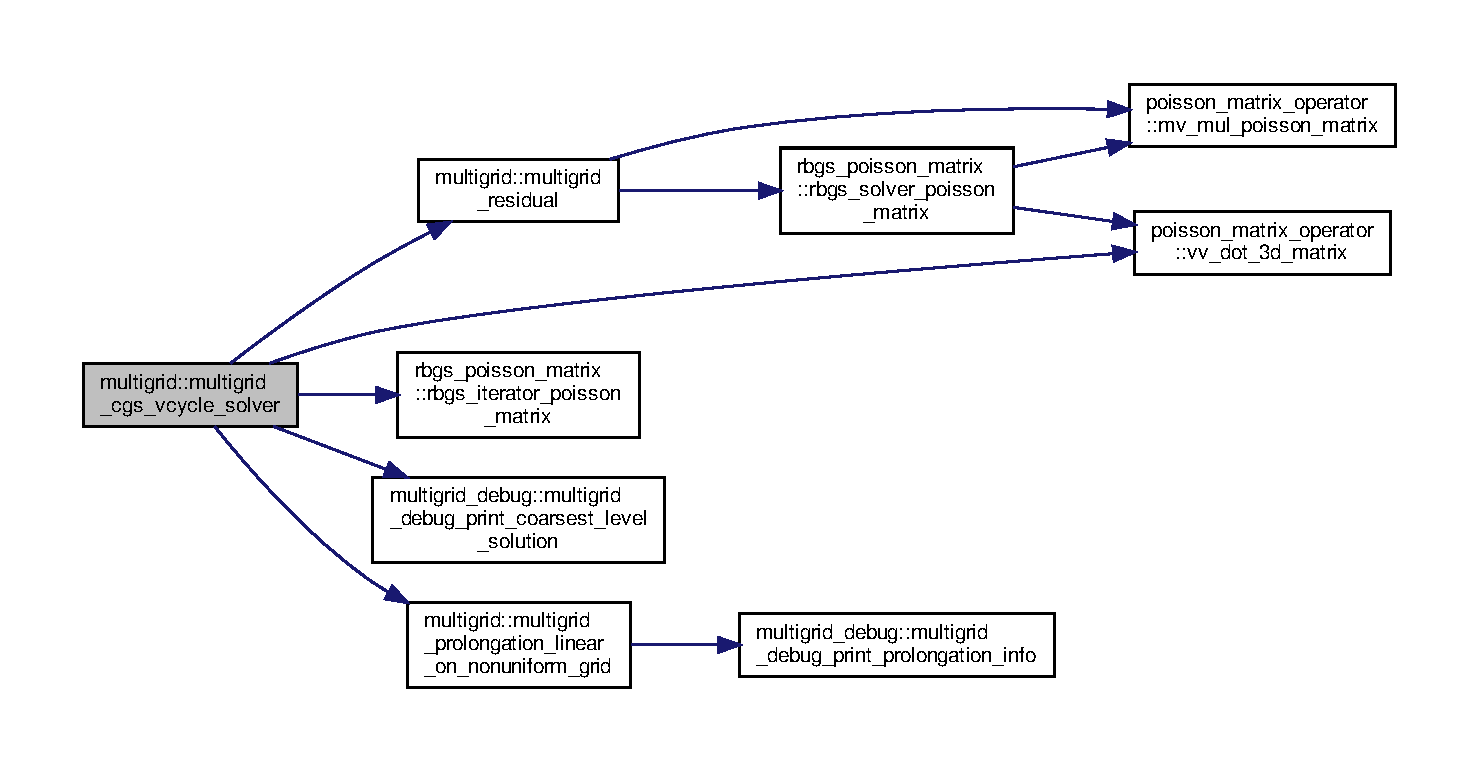
\includegraphics[width=350pt]{namespacemultigrid_aa8278baf0276649fe656c1b8f7dba30a_cgraph}
\end{center}
\end{figure}
Here is the caller graph for this function\+:
\nopagebreak
\begin{figure}[H]
\begin{center}
\leavevmode
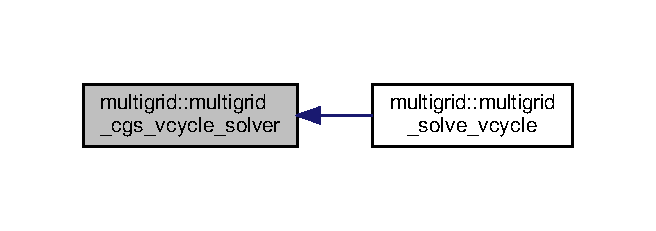
\includegraphics[width=315pt]{namespacemultigrid_aa8278baf0276649fe656c1b8f7dba30a_icgraph}
\end{center}
\end{figure}
\mbox{\Hypertarget{namespacemultigrid_ac8deb32ba5698e37f75c369dc063b277}\label{namespacemultigrid_ac8deb32ba5698e37f75c369dc063b277}} 
\index{multigrid@{multigrid}!multigrid\+\_\+create@{multigrid\+\_\+create}}
\index{multigrid\+\_\+create@{multigrid\+\_\+create}!multigrid@{multigrid}}
\subsubsection{\texorpdfstring{multigrid\+\_\+create()}{multigrid\_create()}}
{\footnotesize\ttfamily subroutine, public multigrid\+::multigrid\+\_\+create (\begin{DoxyParamCaption}\item[{type(\hyperlink{structgeometry_1_1subdomain}{subdomain}), intent(in)}]{sdm,  }\item[{integer(kind=4), intent(in)}]{nlevel,  }\item[{integer(kind=4), intent(in)}]{ncycle,  }\item[{integer(kind=4), intent(in)}]{aggr\+\_\+method,  }\item[{integer(kind=4), intent(in)}]{single\+\_\+aggr\+\_\+level,  }\item[{integer(kind=4), dimension(3), intent(in)}]{adaptive\+\_\+aggr\+\_\+level }\end{DoxyParamCaption})}



Create MG subdomains and Poisson matrix  MG subdomain depends on aggregation type. Different subroutines are called according to aggregation type. 


\begin{DoxyParams}{Parameters}
{\em sdm} & Subdomain \\
\hline
{\em nlevel} & Number of MG level \\
\hline
{\em ncycle} & Number of V-\/cycle \\
\hline
{\em aggr\+\_\+method} & Aggregation method, 0\+: C\+GS, 1\+: C\+GA, 2\+: C\+G\+P\+SA \\
\hline
{\em single\+\_\+aggr\+\_\+level} & Aggregation level for C\+GA \\
\hline
{\em adaptive\+\_\+aggr\+\_\+level} & Aggregation levels in x-\/, y-\/, and z-\/directions for C\+G\+P\+SA \\
\hline
\end{DoxyParams}
Here is the call graph for this function\+:
\nopagebreak
\begin{figure}[H]
\begin{center}
\leavevmode
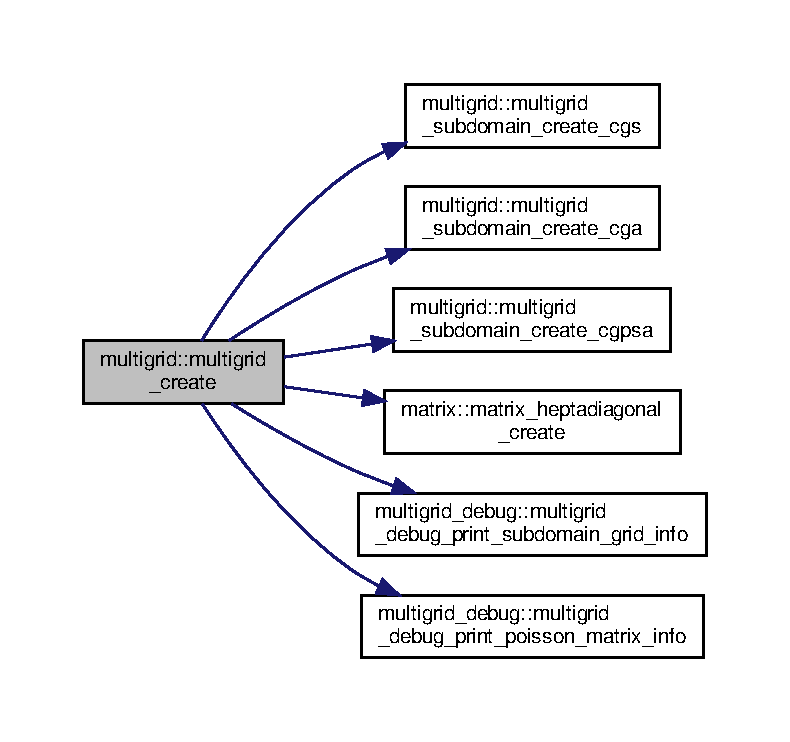
\includegraphics[width=350pt]{namespacemultigrid_ac8deb32ba5698e37f75c369dc063b277_cgraph}
\end{center}
\end{figure}
\mbox{\Hypertarget{namespacemultigrid_a839d1e13e2d0bac4959deec5669d4171}\label{namespacemultigrid_a839d1e13e2d0bac4959deec5669d4171}} 
\index{multigrid@{multigrid}!multigrid\+\_\+prolongation\+\_\+linear\+\_\+on\+\_\+nonuniform\+\_\+grid@{multigrid\+\_\+prolongation\+\_\+linear\+\_\+on\+\_\+nonuniform\+\_\+grid}}
\index{multigrid\+\_\+prolongation\+\_\+linear\+\_\+on\+\_\+nonuniform\+\_\+grid@{multigrid\+\_\+prolongation\+\_\+linear\+\_\+on\+\_\+nonuniform\+\_\+grid}!multigrid@{multigrid}}
\subsubsection{\texorpdfstring{multigrid\+\_\+prolongation\+\_\+linear\+\_\+on\+\_\+nonuniform\+\_\+grid()}{multigrid\_prolongation\_linear\_on\_nonuniform\_grid()}}
{\footnotesize\ttfamily subroutine multigrid\+::multigrid\+\_\+prolongation\+\_\+linear\+\_\+on\+\_\+nonuniform\+\_\+grid (\begin{DoxyParamCaption}\item[{real(kind=8), dimension(0\+:,0\+:,0\+:), intent(out)}]{val\+\_\+f,  }\item[{real(kind=8), dimension(0\+:,0\+:,0\+:), intent(in)}]{val\+\_\+c,  }\item[{type(\hyperlink{structgeometry_1_1subdomain}{subdomain}), intent(in)}]{dm\+\_\+f,  }\item[{type(\hyperlink{structgeometry_1_1subdomain}{subdomain}), intent(in)}]{dm\+\_\+c,  }\item[{integer(kind=4), intent(in)}]{level }\end{DoxyParamCaption})}



Prolongation subroutine for C\+GS, C\+GA, and C\+G\+P\+SA  This subroutine is commonly used by using stride\+\_\+f and offest\+\_\+f variables Constant profile in assumed in finer level. 


\begin{DoxyParams}{Parameters}
{\em val\+\_\+f} & Variable in finer grid \\
\hline
{\em val\+\_\+c} & Variable in coarser grid \\
\hline
{\em dm\+\_\+f} & MG subdomain in finer level \\
\hline
{\em dm\+\_\+c} & MG subdomain in coarser level \\
\hline
{\em level} & MG level where restriction is conducted \\
\hline
\end{DoxyParams}
Here is the call graph for this function\+:
\nopagebreak
\begin{figure}[H]
\begin{center}
\leavevmode
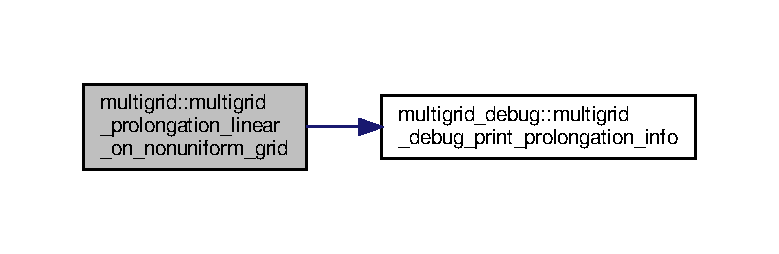
\includegraphics[width=350pt]{namespacemultigrid_a839d1e13e2d0bac4959deec5669d4171_cgraph}
\end{center}
\end{figure}
Here is the caller graph for this function\+:
\nopagebreak
\begin{figure}[H]
\begin{center}
\leavevmode
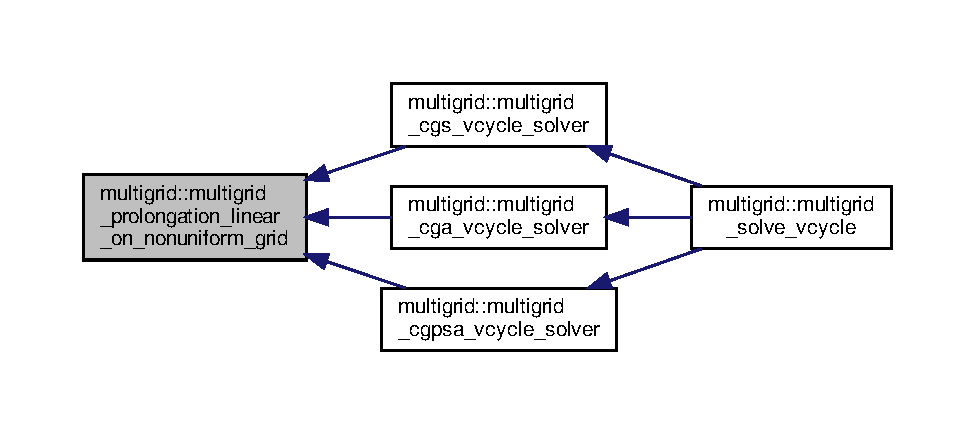
\includegraphics[width=350pt]{namespacemultigrid_a839d1e13e2d0bac4959deec5669d4171_icgraph}
\end{center}
\end{figure}
\mbox{\Hypertarget{namespacemultigrid_ad1ba34848f786afdf0e91afb3d3be819}\label{namespacemultigrid_ad1ba34848f786afdf0e91afb3d3be819}} 
\index{multigrid@{multigrid}!multigrid\+\_\+residual@{multigrid\+\_\+residual}}
\index{multigrid\+\_\+residual@{multigrid\+\_\+residual}!multigrid@{multigrid}}
\subsubsection{\texorpdfstring{multigrid\+\_\+residual()}{multigrid\_residual()}}
{\footnotesize\ttfamily subroutine multigrid\+::multigrid\+\_\+residual (\begin{DoxyParamCaption}\item[{real(kind=8), dimension(0\+:,0\+:,0\+:), intent(out)}]{rsd,  }\item[{type(\hyperlink{structmatrix_1_1matrix__heptadiagonal}{matrix\+\_\+heptadiagonal}), intent(in)}]{a\+\_\+poisson,  }\item[{real(kind=8), dimension(0\+:,0\+:,0\+:), intent(inout)}]{x,  }\item[{real(kind=8), dimension(0\+:,0\+:,0\+:), intent(in)}]{rhs,  }\item[{type(\hyperlink{structgeometry_1_1subdomain}{subdomain}), intent(in)}]{dm,  }\item[{logical, dimension(0\+:2), intent(in)}]{is\+\_\+aggregated }\end{DoxyParamCaption})}



Residual calculation. rsd = rhs -\/ a\+\_\+poisson $\ast$ x. 


\begin{DoxyParams}{Parameters}
{\em rsd} & Residual \\
\hline
{\em a\+\_\+poisson} & A matrix \\
\hline
{\em x} & x vector \\
\hline
{\em rhs} & R\+HS \\
\hline
{\em dm} & MG subdomain in target level \\
\hline
{\em is\+\_\+aggregated} & Aggregation information on whether domain is aggregated (.true.) or not (.false.) \\
\hline
\end{DoxyParams}
Here is the call graph for this function\+:
\nopagebreak
\begin{figure}[H]
\begin{center}
\leavevmode
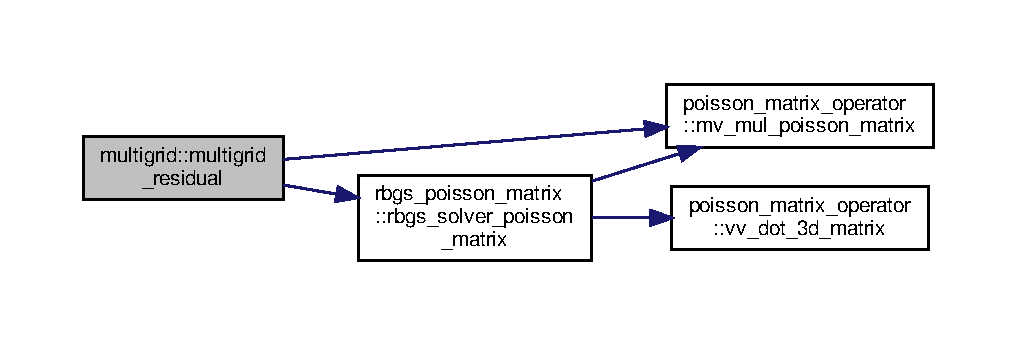
\includegraphics[width=350pt]{namespacemultigrid_ad1ba34848f786afdf0e91afb3d3be819_cgraph}
\end{center}
\end{figure}
Here is the caller graph for this function\+:
\nopagebreak
\begin{figure}[H]
\begin{center}
\leavevmode
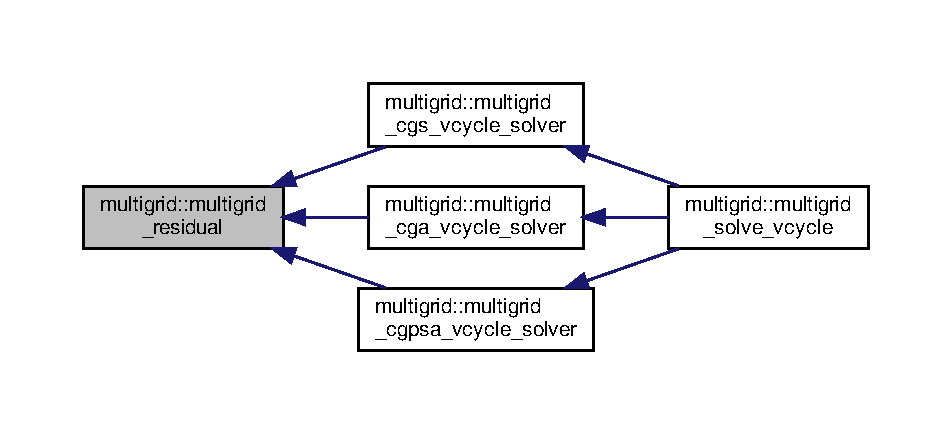
\includegraphics[width=350pt]{namespacemultigrid_ad1ba34848f786afdf0e91afb3d3be819_icgraph}
\end{center}
\end{figure}
\mbox{\Hypertarget{namespacemultigrid_a7d60c9d01777350a79ff7bd975a90121}\label{namespacemultigrid_a7d60c9d01777350a79ff7bd975a90121}} 
\index{multigrid@{multigrid}!multigrid\+\_\+solve\+\_\+vcycle@{multigrid\+\_\+solve\+\_\+vcycle}}
\index{multigrid\+\_\+solve\+\_\+vcycle@{multigrid\+\_\+solve\+\_\+vcycle}!multigrid@{multigrid}}
\subsubsection{\texorpdfstring{multigrid\+\_\+solve\+\_\+vcycle()}{multigrid\_solve\_vcycle()}}
{\footnotesize\ttfamily subroutine, public multigrid\+::multigrid\+\_\+solve\+\_\+vcycle (\begin{DoxyParamCaption}\item[{real(kind=8), dimension(0\+:,0\+:,0\+:), intent(inout)}]{sol,  }\item[{real(kind=8), dimension(0\+:,0\+:,0\+:), intent(inout)}]{rsd,  }\item[{type(\hyperlink{structmatrix_1_1matrix__heptadiagonal}{matrix\+\_\+heptadiagonal}), intent(in)}]{a\+\_\+poisson,  }\item[{real(kind=8), dimension(0\+:,0\+:,0\+:), intent(in)}]{rhs,  }\item[{type(\hyperlink{structgeometry_1_1subdomain}{subdomain}), intent(in)}]{sdm,  }\item[{integer(kind=4), intent(in)}]{maxiteration,  }\item[{real(kind=8), intent(in)}]{tolerance,  }\item[{real(kind=8), intent(in)}]{omega\+\_\+sor }\end{DoxyParamCaption})}



V-\/\+Cycle MG solver\+: call subroutines according to aggregation type. 


\begin{DoxyParams}{Parameters}
{\em sol} & Result solution having a shape of 3D matrix \\
\hline
{\em rsd} & Residual \\
\hline
{\em a\+\_\+poisson} & Heptadiagonal poisson matrix \\
\hline
{\em rhs} & R\+HS vector having a shape of 3D matrix \\
\hline
{\em sdm} & Subdomain \\
\hline
{\em maxiteration} & Maximum number of iterations \\
\hline
{\em tolerance} & Convergence criteria \\
\hline
{\em omega\+\_\+sor} & Relexation factor \\
\hline
\end{DoxyParams}
Here is the call graph for this function\+:
\nopagebreak
\begin{figure}[H]
\begin{center}
\leavevmode
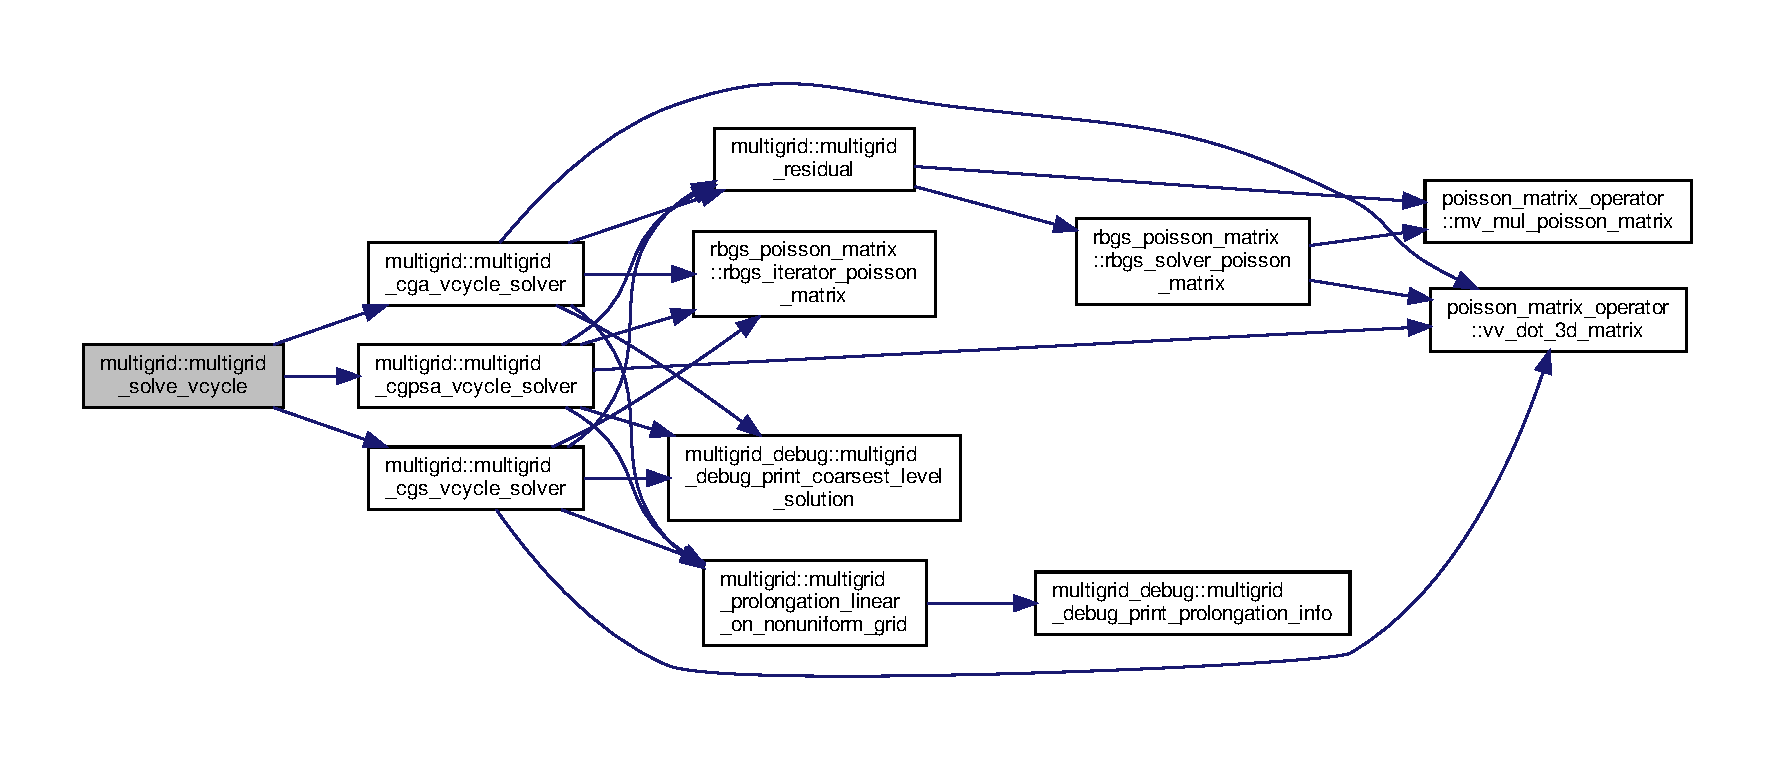
\includegraphics[width=350pt]{namespacemultigrid_a7d60c9d01777350a79ff7bd975a90121_cgraph}
\end{center}
\end{figure}
\mbox{\Hypertarget{namespacemultigrid_ae33e2e076cc087e7d149a3150c1ca1af}\label{namespacemultigrid_ae33e2e076cc087e7d149a3150c1ca1af}} 
\index{multigrid@{multigrid}!multigrid\+\_\+subdomain\+\_\+create\+\_\+cga@{multigrid\+\_\+subdomain\+\_\+create\+\_\+cga}}
\index{multigrid\+\_\+subdomain\+\_\+create\+\_\+cga@{multigrid\+\_\+subdomain\+\_\+create\+\_\+cga}!multigrid@{multigrid}}
\subsubsection{\texorpdfstring{multigrid\+\_\+subdomain\+\_\+create\+\_\+cga()}{multigrid\_subdomain\_create\_cga()}}
{\footnotesize\ttfamily subroutine multigrid\+::multigrid\+\_\+subdomain\+\_\+create\+\_\+cga (\begin{DoxyParamCaption}\item[{type(\hyperlink{structgeometry_1_1subdomain}{subdomain}), intent(in), target}]{sdm }\end{DoxyParamCaption})}



Create MG subdomains for C\+GA  Define MG domain and assign grid dimensions such as mesh size, grid spacing and grid coordinates in each MG levels. 


\begin{DoxyParams}{Parameters}
{\em sdm} & Subdomain \\
\hline
\end{DoxyParams}
Number of grid in aggregation levels, nx $\ast$ number of M\+PI processes

Pointer for mesh size in current MG level

Pointer for grid spacing in current MG level

Pointer for grid coordinates in current MG levelHere is the caller graph for this function\+:
\nopagebreak
\begin{figure}[H]
\begin{center}
\leavevmode
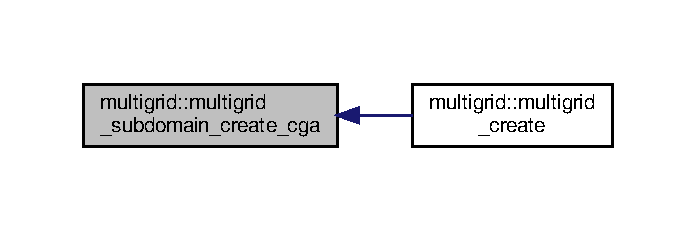
\includegraphics[width=334pt]{namespacemultigrid_ae33e2e076cc087e7d149a3150c1ca1af_icgraph}
\end{center}
\end{figure}
\mbox{\Hypertarget{namespacemultigrid_aa2eb7c900fb5875f844c04c27c552373}\label{namespacemultigrid_aa2eb7c900fb5875f844c04c27c552373}} 
\index{multigrid@{multigrid}!multigrid\+\_\+subdomain\+\_\+create\+\_\+cgpsa@{multigrid\+\_\+subdomain\+\_\+create\+\_\+cgpsa}}
\index{multigrid\+\_\+subdomain\+\_\+create\+\_\+cgpsa@{multigrid\+\_\+subdomain\+\_\+create\+\_\+cgpsa}!multigrid@{multigrid}}
\subsubsection{\texorpdfstring{multigrid\+\_\+subdomain\+\_\+create\+\_\+cgpsa()}{multigrid\_subdomain\_create\_cgpsa()}}
{\footnotesize\ttfamily subroutine multigrid\+::multigrid\+\_\+subdomain\+\_\+create\+\_\+cgpsa (\begin{DoxyParamCaption}\item[{type(\hyperlink{structgeometry_1_1subdomain}{subdomain}), intent(in), target}]{sdm }\end{DoxyParamCaption})}



Create MG subdomains for C\+G\+P\+SA  Define MG domain and assign grid dimensions such as mesh size, grid spacing and grid coordinates in each MG levels. 


\begin{DoxyParams}{Parameters}
{\em sdm} & Subdomain \\
\hline
\end{DoxyParams}
Number of grid in aggregation levels, nx $\ast$ number of M\+PI processes

Pointer for mesh size in current MG level

Pointer for grid spacing in current MG level

Pointer for grid coordinates in current MG levelHere is the caller graph for this function\+:
\nopagebreak
\begin{figure}[H]
\begin{center}
\leavevmode
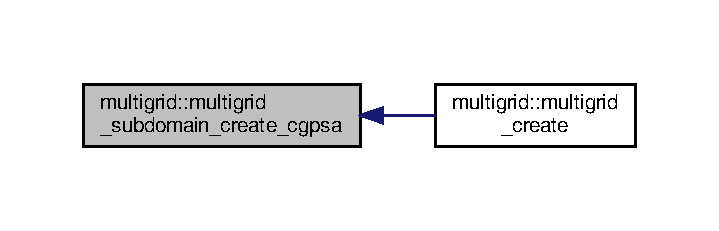
\includegraphics[width=345pt]{namespacemultigrid_aa2eb7c900fb5875f844c04c27c552373_icgraph}
\end{center}
\end{figure}
\mbox{\Hypertarget{namespacemultigrid_acb52ce247bf637e69274d8da44d1f159}\label{namespacemultigrid_acb52ce247bf637e69274d8da44d1f159}} 
\index{multigrid@{multigrid}!multigrid\+\_\+subdomain\+\_\+create\+\_\+cgs@{multigrid\+\_\+subdomain\+\_\+create\+\_\+cgs}}
\index{multigrid\+\_\+subdomain\+\_\+create\+\_\+cgs@{multigrid\+\_\+subdomain\+\_\+create\+\_\+cgs}!multigrid@{multigrid}}
\subsubsection{\texorpdfstring{multigrid\+\_\+subdomain\+\_\+create\+\_\+cgs()}{multigrid\_subdomain\_create\_cgs()}}
{\footnotesize\ttfamily subroutine multigrid\+::multigrid\+\_\+subdomain\+\_\+create\+\_\+cgs (\begin{DoxyParamCaption}\item[{type(\hyperlink{structgeometry_1_1subdomain}{subdomain}), intent(in), target}]{sdm }\end{DoxyParamCaption})}



Create MG subdomains for C\+GS  Define MG domain and assign grid dimensions such as mesh size, grid spacing and grid coordinates in each MG levels. 


\begin{DoxyParams}{Parameters}
{\em sdm} & Subdomain \\
\hline
\end{DoxyParams}
Pointer for mesh size in current MG level

Pointer for grid spacing in current MG level

Pointer for grid coordinates in current MG levelHere is the caller graph for this function\+:
\nopagebreak
\begin{figure}[H]
\begin{center}
\leavevmode
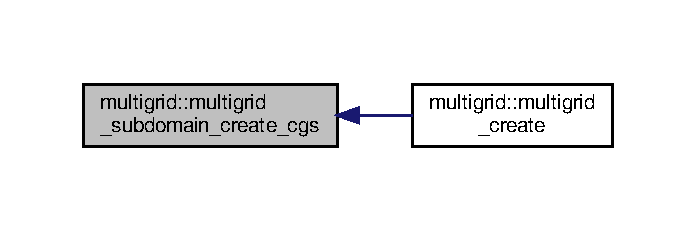
\includegraphics[width=334pt]{namespacemultigrid_acb52ce247bf637e69274d8da44d1f159_icgraph}
\end{center}
\end{figure}

\hypertarget{namespacemultigrid__debug}{}\section{multigrid\+\_\+debug Module Reference}
\label{namespacemultigrid__debug}\index{multigrid\+\_\+debug@{multigrid\+\_\+debug}}


Module for printing multigrid information for debugging.  


\subsection*{Functions/\+Subroutines}
\begin{DoxyCompactItemize}
\item 
subroutine, public \hyperlink{namespacemultigrid__debug_aa5dcd15e32c5dc719638263835c5ed43}{multigrid\+\_\+debug\+\_\+print\+\_\+subdomain\+\_\+grid\+\_\+info} (sdm, mg\+\_\+sdm, n\+\_\+levels)
\begin{DoxyCompactList}\small\item\em Print the grid information. \end{DoxyCompactList}\item 
subroutine, public \hyperlink{namespacemultigrid__debug_aae55d6fc6a22d97825619d5bb58a1b88}{multigrid\+\_\+debug\+\_\+print\+\_\+poisson\+\_\+matrix\+\_\+info} (mg\+\_\+sdm, mg\+\_\+a\+\_\+poisson, lv)
\begin{DoxyCompactList}\small\item\em Print the poisson matrix info in multigrid levels. \end{DoxyCompactList}\item 
subroutine, public \hyperlink{namespacemultigrid__debug_a99e36a8239b91fbf3681cd88ab8f06dd}{multigrid\+\_\+debug\+\_\+print\+\_\+restriction\+\_\+info} (val\+\_\+c, val\+\_\+f, vol\+\_\+c, vol\+\_\+f, level, nx\+\_\+c, ny\+\_\+c, nz\+\_\+c, i\+\_\+stride\+\_\+f, j\+\_\+stride\+\_\+f, k\+\_\+stride\+\_\+f, i\+\_\+offset\+\_\+f, j\+\_\+offset\+\_\+f, k\+\_\+offset\+\_\+f)
\begin{DoxyCompactList}\small\item\em Print the restriction results from finer grid to coarser grid. \end{DoxyCompactList}\item 
subroutine, public \hyperlink{namespacemultigrid__debug_a4e9617a0cc65c4169970f289117de416}{multigrid\+\_\+debug\+\_\+print\+\_\+prolongation\+\_\+info} (val\+\_\+c, val\+\_\+f, level, nx\+\_\+f, ny\+\_\+f, nz\+\_\+f, i\+\_\+stride\+\_\+f, j\+\_\+stride\+\_\+f, k\+\_\+stride\+\_\+f, i\+\_\+offset\+\_\+f, j\+\_\+offset\+\_\+f, k\+\_\+offset\+\_\+f)
\begin{DoxyCompactList}\small\item\em Print the prolongation results from coarser grid to finer grid. \end{DoxyCompactList}\item 
subroutine, public \hyperlink{namespacemultigrid__debug_ad5c036138c7fd5e103641a667a88e6cf}{multigrid\+\_\+debug\+\_\+print\+\_\+coarsest\+\_\+level\+\_\+solution} (cyc, mg\+\_\+sdm)
\begin{DoxyCompactList}\small\item\em Print the solution in the coarsest level. \end{DoxyCompactList}\end{DoxyCompactItemize}


\subsection{Detailed Description}
Module for printing multigrid information for debugging. 

\subsection{Function/\+Subroutine Documentation}
\mbox{\Hypertarget{namespacemultigrid__debug_ad5c036138c7fd5e103641a667a88e6cf}\label{namespacemultigrid__debug_ad5c036138c7fd5e103641a667a88e6cf}} 
\index{multigrid\+\_\+debug@{multigrid\+\_\+debug}!multigrid\+\_\+debug\+\_\+print\+\_\+coarsest\+\_\+level\+\_\+solution@{multigrid\+\_\+debug\+\_\+print\+\_\+coarsest\+\_\+level\+\_\+solution}}
\index{multigrid\+\_\+debug\+\_\+print\+\_\+coarsest\+\_\+level\+\_\+solution@{multigrid\+\_\+debug\+\_\+print\+\_\+coarsest\+\_\+level\+\_\+solution}!multigrid\+\_\+debug@{multigrid\+\_\+debug}}
\subsubsection{\texorpdfstring{multigrid\+\_\+debug\+\_\+print\+\_\+coarsest\+\_\+level\+\_\+solution()}{multigrid\_debug\_print\_coarsest\_level\_solution()}}
{\footnotesize\ttfamily subroutine, public multigrid\+\_\+debug\+::multigrid\+\_\+debug\+\_\+print\+\_\+coarsest\+\_\+level\+\_\+solution (\begin{DoxyParamCaption}\item[{integer(kind=4), intent(in)}]{cyc,  }\item[{type(\hyperlink{structgeometry_1_1subdomain}{subdomain}), intent(in)}]{mg\+\_\+sdm }\end{DoxyParamCaption})}



Print the solution in the coarsest level. 


\begin{DoxyParams}{Parameters}
{\em cyc} & V-\/cycle number \\
\hline
{\em mg\+\_\+sdm} & Target multigrid subdomain \\
\hline
\end{DoxyParams}
Here is the caller graph for this function\+:
\nopagebreak
\begin{figure}[H]
\begin{center}
\leavevmode
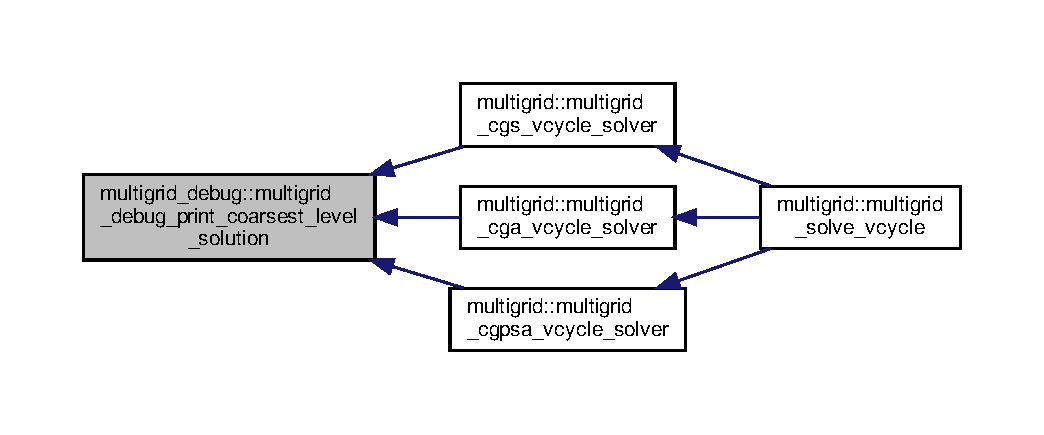
\includegraphics[width=350pt]{namespacemultigrid__debug_ad5c036138c7fd5e103641a667a88e6cf_icgraph}
\end{center}
\end{figure}
\mbox{\Hypertarget{namespacemultigrid__debug_aae55d6fc6a22d97825619d5bb58a1b88}\label{namespacemultigrid__debug_aae55d6fc6a22d97825619d5bb58a1b88}} 
\index{multigrid\+\_\+debug@{multigrid\+\_\+debug}!multigrid\+\_\+debug\+\_\+print\+\_\+poisson\+\_\+matrix\+\_\+info@{multigrid\+\_\+debug\+\_\+print\+\_\+poisson\+\_\+matrix\+\_\+info}}
\index{multigrid\+\_\+debug\+\_\+print\+\_\+poisson\+\_\+matrix\+\_\+info@{multigrid\+\_\+debug\+\_\+print\+\_\+poisson\+\_\+matrix\+\_\+info}!multigrid\+\_\+debug@{multigrid\+\_\+debug}}
\subsubsection{\texorpdfstring{multigrid\+\_\+debug\+\_\+print\+\_\+poisson\+\_\+matrix\+\_\+info()}{multigrid\_debug\_print\_poisson\_matrix\_info()}}
{\footnotesize\ttfamily subroutine, public multigrid\+\_\+debug\+::multigrid\+\_\+debug\+\_\+print\+\_\+poisson\+\_\+matrix\+\_\+info (\begin{DoxyParamCaption}\item[{type(\hyperlink{structgeometry_1_1subdomain}{subdomain}), intent(in)}]{mg\+\_\+sdm,  }\item[{type(\hyperlink{structmatrix_1_1matrix__heptadiagonal}{matrix\+\_\+heptadiagonal}), intent(in)}]{mg\+\_\+a\+\_\+poisson,  }\item[{integer(kind=4), intent(in)}]{lv }\end{DoxyParamCaption})}



Print the poisson matrix info in multigrid levels. 


\begin{DoxyParams}{Parameters}
{\em mg\+\_\+sdm} & Target multigrid subdomain \\
\hline
{\em mg\+\_\+a\+\_\+poisson} & Target Poisson matrix in multigrid level \\
\hline
{\em lv} & Target multigrid level \\
\hline
\end{DoxyParams}
Here is the caller graph for this function\+:
\nopagebreak
\begin{figure}[H]
\begin{center}
\leavevmode
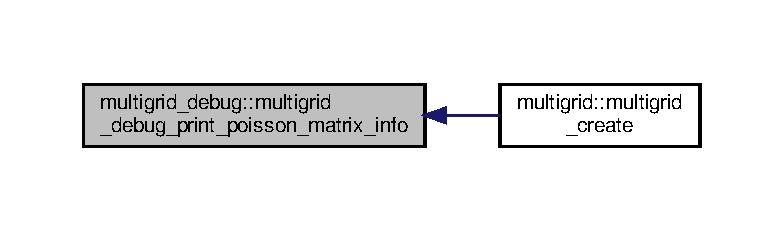
\includegraphics[width=350pt]{namespacemultigrid__debug_aae55d6fc6a22d97825619d5bb58a1b88_icgraph}
\end{center}
\end{figure}
\mbox{\Hypertarget{namespacemultigrid__debug_a4e9617a0cc65c4169970f289117de416}\label{namespacemultigrid__debug_a4e9617a0cc65c4169970f289117de416}} 
\index{multigrid\+\_\+debug@{multigrid\+\_\+debug}!multigrid\+\_\+debug\+\_\+print\+\_\+prolongation\+\_\+info@{multigrid\+\_\+debug\+\_\+print\+\_\+prolongation\+\_\+info}}
\index{multigrid\+\_\+debug\+\_\+print\+\_\+prolongation\+\_\+info@{multigrid\+\_\+debug\+\_\+print\+\_\+prolongation\+\_\+info}!multigrid\+\_\+debug@{multigrid\+\_\+debug}}
\subsubsection{\texorpdfstring{multigrid\+\_\+debug\+\_\+print\+\_\+prolongation\+\_\+info()}{multigrid\_debug\_print\_prolongation\_info()}}
{\footnotesize\ttfamily subroutine, public multigrid\+\_\+debug\+::multigrid\+\_\+debug\+\_\+print\+\_\+prolongation\+\_\+info (\begin{DoxyParamCaption}\item[{real(kind=8), dimension(0\+:,0\+:,0\+:), intent(in)}]{val\+\_\+c,  }\item[{real(kind=8), dimension(0\+:,0\+:,0\+:), intent(in)}]{val\+\_\+f,  }\item[{integer(kind=4), intent(in)}]{level,  }\item[{integer(kind=4), intent(in)}]{nx\+\_\+f,  }\item[{integer(kind=4), intent(in)}]{ny\+\_\+f,  }\item[{integer(kind=4), intent(in)}]{nz\+\_\+f,  }\item[{integer(kind=4), intent(in)}]{i\+\_\+stride\+\_\+f,  }\item[{integer(kind=4), intent(in)}]{j\+\_\+stride\+\_\+f,  }\item[{integer(kind=4), intent(in)}]{k\+\_\+stride\+\_\+f,  }\item[{integer(kind=4), intent(in)}]{i\+\_\+offset\+\_\+f,  }\item[{integer(kind=4), intent(in)}]{j\+\_\+offset\+\_\+f,  }\item[{integer(kind=4), intent(in)}]{k\+\_\+offset\+\_\+f }\end{DoxyParamCaption})}



Print the prolongation results from coarser grid to finer grid. 


\begin{DoxyParams}{Parameters}
{\em val\+\_\+c} & grid variables in coarser grid \\
\hline
{\em val\+\_\+f} & grid variables in finer grid \\
\hline
{\em level} & Restriction level \\
\hline
{\em nx\+\_\+c} & Number of grids in coarser grid in x-\/direction \\
\hline
{\em ny\+\_\+c} & Number of grids in coarser grid in y-\/direction \\
\hline
{\em nz\+\_\+c} & Number of grids in coarser grid in z-\/direction \\
\hline
{\em i\+\_\+stride\+\_\+f} & 2 if not aggretated, 1 if aggregated \\
\hline
{\em j\+\_\+stride\+\_\+f} & 2 if not aggretated, 1 if aggregated \\
\hline
{\em k\+\_\+stride\+\_\+f} & 2 if not aggretated, 1 if aggregated \\
\hline
{\em i\+\_\+offset\+\_\+f} & 1 if not aggretated, 0 if aggregated \\
\hline
{\em j\+\_\+offset\+\_\+f} & 1 if not aggretated, 0 if aggregated \\
\hline
{\em k\+\_\+offset\+\_\+f} & 1 if not aggretated, 0 if aggregated \\
\hline
\end{DoxyParams}
Here is the caller graph for this function\+:
\nopagebreak
\begin{figure}[H]
\begin{center}
\leavevmode
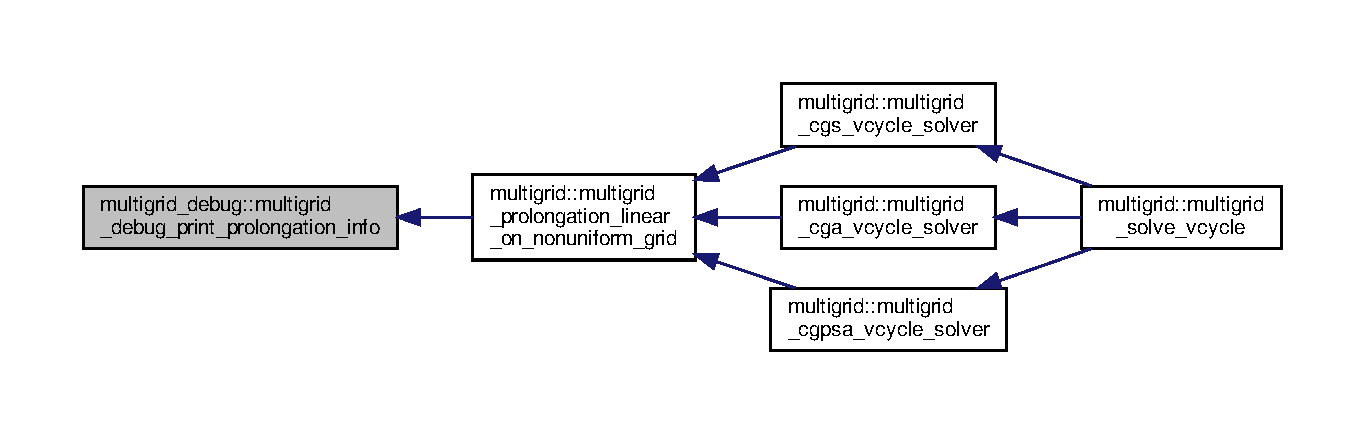
\includegraphics[width=350pt]{namespacemultigrid__debug_a4e9617a0cc65c4169970f289117de416_icgraph}
\end{center}
\end{figure}
\mbox{\Hypertarget{namespacemultigrid__debug_a99e36a8239b91fbf3681cd88ab8f06dd}\label{namespacemultigrid__debug_a99e36a8239b91fbf3681cd88ab8f06dd}} 
\index{multigrid\+\_\+debug@{multigrid\+\_\+debug}!multigrid\+\_\+debug\+\_\+print\+\_\+restriction\+\_\+info@{multigrid\+\_\+debug\+\_\+print\+\_\+restriction\+\_\+info}}
\index{multigrid\+\_\+debug\+\_\+print\+\_\+restriction\+\_\+info@{multigrid\+\_\+debug\+\_\+print\+\_\+restriction\+\_\+info}!multigrid\+\_\+debug@{multigrid\+\_\+debug}}
\subsubsection{\texorpdfstring{multigrid\+\_\+debug\+\_\+print\+\_\+restriction\+\_\+info()}{multigrid\_debug\_print\_restriction\_info()}}
{\footnotesize\ttfamily subroutine, public multigrid\+\_\+debug\+::multigrid\+\_\+debug\+\_\+print\+\_\+restriction\+\_\+info (\begin{DoxyParamCaption}\item[{real(kind=8), dimension(0\+:,0\+:,0\+:), intent(in)}]{val\+\_\+c,  }\item[{real(kind=8), dimension(0\+:,0\+:,0\+:), intent(in)}]{val\+\_\+f,  }\item[{real(kind=8), intent(in)}]{vol\+\_\+c,  }\item[{real(kind=8), dimension(2,2,2), intent(in)}]{vol\+\_\+f,  }\item[{integer(kind=4), intent(in)}]{level,  }\item[{integer(kind=4), intent(in)}]{nx\+\_\+c,  }\item[{integer(kind=4), intent(in)}]{ny\+\_\+c,  }\item[{integer(kind=4), intent(in)}]{nz\+\_\+c,  }\item[{integer(kind=4), intent(in)}]{i\+\_\+stride\+\_\+f,  }\item[{integer(kind=4), intent(in)}]{j\+\_\+stride\+\_\+f,  }\item[{integer(kind=4), intent(in)}]{k\+\_\+stride\+\_\+f,  }\item[{integer(kind=4), intent(in)}]{i\+\_\+offset\+\_\+f,  }\item[{integer(kind=4), intent(in)}]{j\+\_\+offset\+\_\+f,  }\item[{integer(kind=4), intent(in)}]{k\+\_\+offset\+\_\+f }\end{DoxyParamCaption})}



Print the restriction results from finer grid to coarser grid. 


\begin{DoxyParams}{Parameters}
{\em val\+\_\+c} & grid variables in coarser grid \\
\hline
{\em val\+\_\+f} & grid variables in finer grid \\
\hline
{\em vol\+\_\+c} & grid volume in coarser level (1x1x1) \\
\hline
{\em vol\+\_\+f} & grid volume in finer level (2x2x2) \\
\hline
{\em level} & Restriction level \\
\hline
{\em nx\+\_\+c} & Number of grids in coarser grid in x-\/direction \\
\hline
{\em ny\+\_\+c} & Number of grids in coarser grid in y-\/direction \\
\hline
{\em nz\+\_\+c} & Number of grids in coarser grid in z-\/direction \\
\hline
{\em i\+\_\+stride\+\_\+f} & 2 if not aggretated, 1 if aggregated \\
\hline
{\em j\+\_\+stride\+\_\+f} & 2 if not aggretated, 1 if aggregated \\
\hline
{\em k\+\_\+stride\+\_\+f} & 2 if not aggretated, 1 if aggregated \\
\hline
{\em i\+\_\+offset\+\_\+f} & 1 if not aggretated, 0 if aggregated \\
\hline
{\em j\+\_\+offset\+\_\+f} & 1 if not aggretated, 0 if aggregated \\
\hline
{\em k\+\_\+offset\+\_\+f} & 1 if not aggretated, 0 if aggregated \\
\hline
\end{DoxyParams}
Here is the caller graph for this function\+:
\nopagebreak
\begin{figure}[H]
\begin{center}
\leavevmode
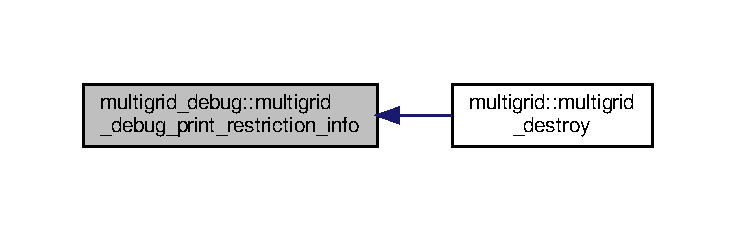
\includegraphics[width=350pt]{namespacemultigrid__debug_a99e36a8239b91fbf3681cd88ab8f06dd_icgraph}
\end{center}
\end{figure}
\mbox{\Hypertarget{namespacemultigrid__debug_aa5dcd15e32c5dc719638263835c5ed43}\label{namespacemultigrid__debug_aa5dcd15e32c5dc719638263835c5ed43}} 
\index{multigrid\+\_\+debug@{multigrid\+\_\+debug}!multigrid\+\_\+debug\+\_\+print\+\_\+subdomain\+\_\+grid\+\_\+info@{multigrid\+\_\+debug\+\_\+print\+\_\+subdomain\+\_\+grid\+\_\+info}}
\index{multigrid\+\_\+debug\+\_\+print\+\_\+subdomain\+\_\+grid\+\_\+info@{multigrid\+\_\+debug\+\_\+print\+\_\+subdomain\+\_\+grid\+\_\+info}!multigrid\+\_\+debug@{multigrid\+\_\+debug}}
\subsubsection{\texorpdfstring{multigrid\+\_\+debug\+\_\+print\+\_\+subdomain\+\_\+grid\+\_\+info()}{multigrid\_debug\_print\_subdomain\_grid\_info()}}
{\footnotesize\ttfamily subroutine, public multigrid\+\_\+debug\+::multigrid\+\_\+debug\+\_\+print\+\_\+subdomain\+\_\+grid\+\_\+info (\begin{DoxyParamCaption}\item[{type(\hyperlink{structgeometry_1_1subdomain}{subdomain}), intent(in)}]{sdm,  }\item[{type(\hyperlink{structgeometry_1_1subdomain}{subdomain}), dimension(\+:), intent(in)}]{mg\+\_\+sdm,  }\item[{integer(kind=4), intent(in)}]{n\+\_\+levels }\end{DoxyParamCaption})}



Print the grid information. 


\begin{DoxyParams}{Parameters}
{\em sdm} & Subdomain \\
\hline
{\em mg\+\_\+sdm} & Multigrid subdomains \\
\hline
{\em n\+\_\+levels} & Number of multigrid levels \\
\hline
\end{DoxyParams}
Here is the caller graph for this function\+:
\nopagebreak
\begin{figure}[H]
\begin{center}
\leavevmode
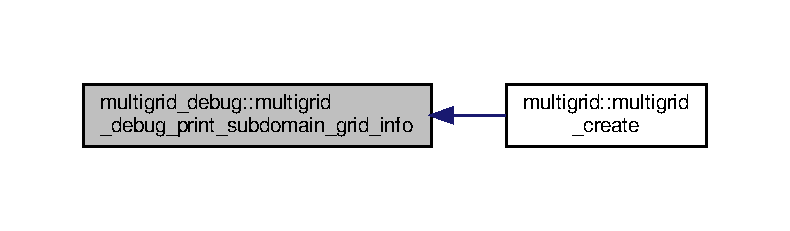
\includegraphics[width=350pt]{namespacemultigrid__debug_aa5dcd15e32c5dc719638263835c5ed43_icgraph}
\end{center}
\end{figure}

\hypertarget{namespacepoisson__matrix__operator}{}\section{poisson\+\_\+matrix\+\_\+operator Module Reference}
\label{namespacepoisson__matrix__operator}\index{poisson\+\_\+matrix\+\_\+operator@{poisson\+\_\+matrix\+\_\+operator}}


Module for matrix operations of heptadiagonal poisson matrix.  


\subsection*{Functions/\+Subroutines}
\begin{DoxyCompactItemize}
\item 
subroutine, public \hyperlink{namespacepoisson__matrix__operator_a10219d15282e48b5afab88408912fb2f}{vv\+\_\+dot\+\_\+3d\+\_\+matrix} (result, x, y, nx, ny, nz, is\+\_\+serial)
\begin{DoxyCompactList}\small\item\em Inner product for 3D matrix x and 3D matrix y. A 3D matrix is treated as a vector. \end{DoxyCompactList}\item 
subroutine, public \hyperlink{namespacepoisson__matrix__operator_a0a0591ff6a44595b830d4d0655e25106}{mv\+\_\+mul\+\_\+poisson\+\_\+matrix} (y, a\+\_\+poisson, x, dm, is\+\_\+serial)
\begin{DoxyCompactList}\small\item\em MV multiplication for heptadiagonal poisson matrix a\+\_\+poisson and 3D matrix x 3D matrix is treated as a vector and poisson matrix is treated as a matrix. \end{DoxyCompactList}\end{DoxyCompactItemize}


\subsection{Detailed Description}
Module for matrix operations of heptadiagonal poisson matrix. 

MV multiplication and VV inner product 

\subsection{Function/\+Subroutine Documentation}
\mbox{\Hypertarget{namespacepoisson__matrix__operator_a0a0591ff6a44595b830d4d0655e25106}\label{namespacepoisson__matrix__operator_a0a0591ff6a44595b830d4d0655e25106}} 
\index{poisson\+\_\+matrix\+\_\+operator@{poisson\+\_\+matrix\+\_\+operator}!mv\+\_\+mul\+\_\+poisson\+\_\+matrix@{mv\+\_\+mul\+\_\+poisson\+\_\+matrix}}
\index{mv\+\_\+mul\+\_\+poisson\+\_\+matrix@{mv\+\_\+mul\+\_\+poisson\+\_\+matrix}!poisson\+\_\+matrix\+\_\+operator@{poisson\+\_\+matrix\+\_\+operator}}
\subsubsection{\texorpdfstring{mv\+\_\+mul\+\_\+poisson\+\_\+matrix()}{mv\_mul\_poisson\_matrix()}}
{\footnotesize\ttfamily subroutine, public poisson\+\_\+matrix\+\_\+operator\+::mv\+\_\+mul\+\_\+poisson\+\_\+matrix (\begin{DoxyParamCaption}\item[{real(kind=8), dimension(0\+:,0\+:,0\+:), intent(out)}]{y,  }\item[{type(\hyperlink{structmatrix_1_1matrix__heptadiagonal}{matrix\+\_\+heptadiagonal}), intent(in)}]{a\+\_\+poisson,  }\item[{real(kind=8), dimension(0\+:,0\+:,0\+:), intent(inout)}]{x,  }\item[{type(\hyperlink{structgeometry_1_1subdomain}{subdomain}), intent(in)}]{dm,  }\item[{logical, dimension(0\+:2), intent(in)}]{is\+\_\+serial }\end{DoxyParamCaption})}



MV multiplication for heptadiagonal poisson matrix a\+\_\+poisson and 3D matrix x 3D matrix is treated as a vector and poisson matrix is treated as a matrix. 


\begin{DoxyParams}{Parameters}
{\em y} & MV result 3D matrix \\
\hline
{\em a\+\_\+poisson} & Heptadiagonal poisson matrix \\
\hline
{\em x} & 3D matrix x \\
\hline
{\em dm} & Subdomain \\
\hline
{\em is\+\_\+serial} & Boolean whether domain is aggregated (.true.) or not (.false.) (aggregated = serial) \\
\hline
\end{DoxyParams}
Here is the caller graph for this function\+:
\nopagebreak
\begin{figure}[H]
\begin{center}
\leavevmode
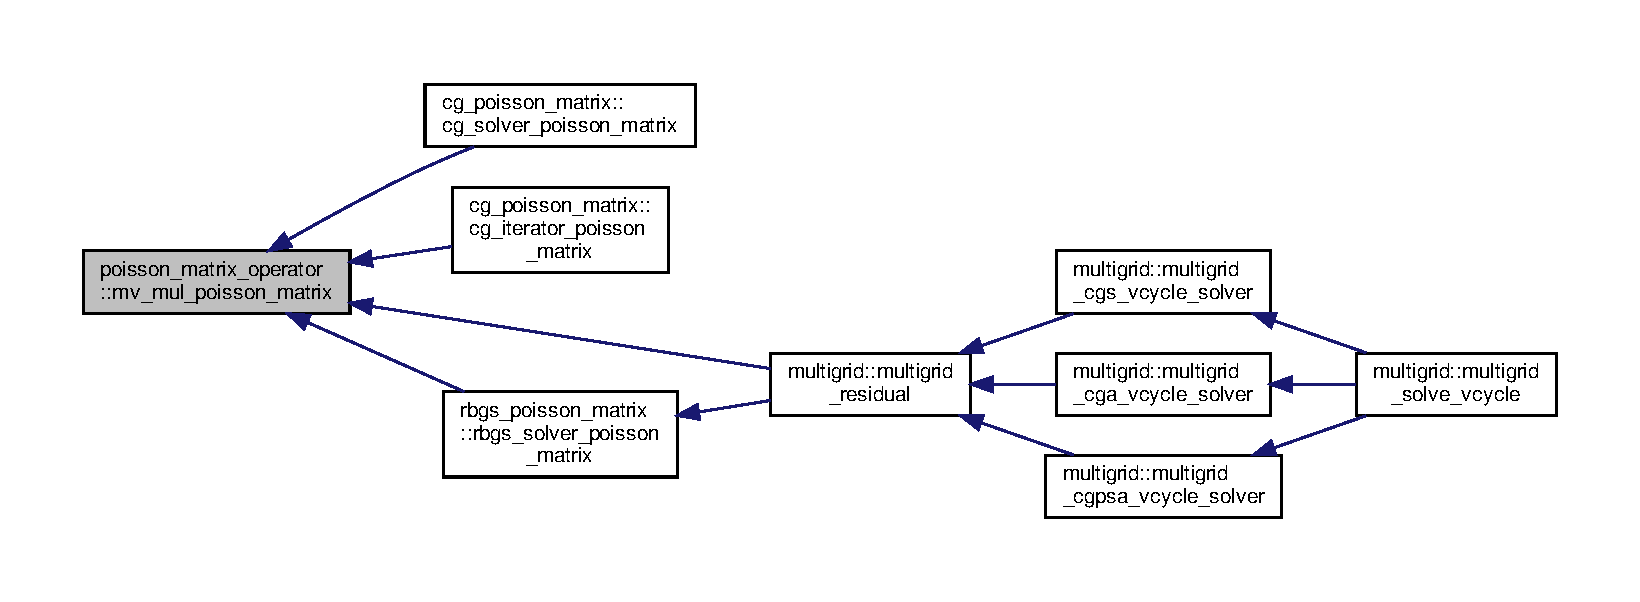
\includegraphics[width=350pt]{namespacepoisson__matrix__operator_a0a0591ff6a44595b830d4d0655e25106_icgraph}
\end{center}
\end{figure}
\mbox{\Hypertarget{namespacepoisson__matrix__operator_a10219d15282e48b5afab88408912fb2f}\label{namespacepoisson__matrix__operator_a10219d15282e48b5afab88408912fb2f}} 
\index{poisson\+\_\+matrix\+\_\+operator@{poisson\+\_\+matrix\+\_\+operator}!vv\+\_\+dot\+\_\+3d\+\_\+matrix@{vv\+\_\+dot\+\_\+3d\+\_\+matrix}}
\index{vv\+\_\+dot\+\_\+3d\+\_\+matrix@{vv\+\_\+dot\+\_\+3d\+\_\+matrix}!poisson\+\_\+matrix\+\_\+operator@{poisson\+\_\+matrix\+\_\+operator}}
\subsubsection{\texorpdfstring{vv\+\_\+dot\+\_\+3d\+\_\+matrix()}{vv\_dot\_3d\_matrix()}}
{\footnotesize\ttfamily subroutine, public poisson\+\_\+matrix\+\_\+operator\+::vv\+\_\+dot\+\_\+3d\+\_\+matrix (\begin{DoxyParamCaption}\item[{real(kind=8), intent(out)}]{result,  }\item[{real(kind=8), dimension(0\+:,0\+:,0\+:), intent(in)}]{x,  }\item[{real(kind=8), dimension(0\+:,0\+:,0\+:), intent(in)}]{y,  }\item[{integer(kind=4), intent(in)}]{nx,  }\item[{integer(kind=4), intent(in)}]{ny,  }\item[{integer(kind=4), intent(in)}]{nz,  }\item[{logical, dimension(0\+:2), intent(in)}]{is\+\_\+serial }\end{DoxyParamCaption})}



Inner product for 3D matrix x and 3D matrix y. A 3D matrix is treated as a vector. 


\begin{DoxyParams}{Parameters}
{\em result} & Inner product result \\
\hline
{\em x} & 3D matrix x \\
\hline
{\em y} & 3D matrix y \\
\hline
{\em nx} & Size of 3D matrix in x-\/direction \\
\hline
{\em ny} & Size of 3D matrix in y-\/direction \\
\hline
{\em nz} & Size of 3D matrix in z-\/direction \\
\hline
{\em is\+\_\+serial} & Boolean whether domain is aggregated (.true.) or not (.false.) (aggregated = serial) \\
\hline
\end{DoxyParams}
Here is the caller graph for this function\+:
\nopagebreak
\begin{figure}[H]
\begin{center}
\leavevmode
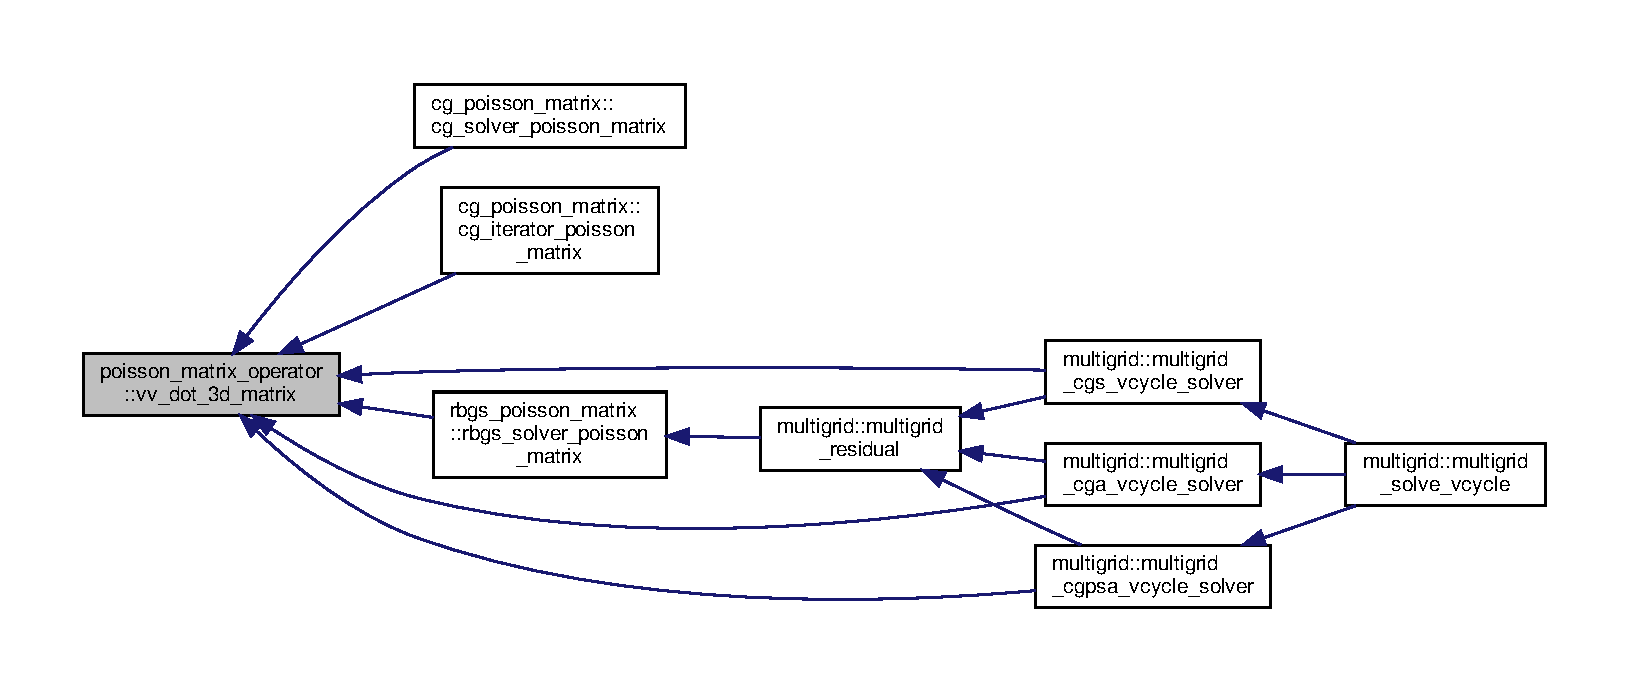
\includegraphics[width=350pt]{namespacepoisson__matrix__operator_a10219d15282e48b5afab88408912fb2f_icgraph}
\end{center}
\end{figure}

\hypertarget{namespacerbgs__poisson__matrix}{}\section{rbgs\+\_\+poisson\+\_\+matrix Module Reference}
\label{namespacerbgs__poisson__matrix}\index{rbgs\+\_\+poisson\+\_\+matrix@{rbgs\+\_\+poisson\+\_\+matrix}}


Module for for red-\/black Gauss-\/\+Seidel method with heptadiagonal poisson matrix.  


\subsection*{Functions/\+Subroutines}
\begin{DoxyCompactItemize}
\item 
subroutine, public \hyperlink{namespacerbgs__poisson__matrix_a4706c96056deda74122016f5c07ba337}{rbgs\+\_\+solver\+\_\+poisson\+\_\+matrix} (sol, a\+\_\+poisson, rhs, dm, maxiteration, tolerance, omega, is\+\_\+aggregated)
\begin{DoxyCompactList}\small\item\em Red-\/black Gauss-\/\+Seidel solver with convergence criteria. \end{DoxyCompactList}\item 
subroutine, public \hyperlink{namespacerbgs__poisson__matrix_a35a0647dd0b1e09cb482bde7fba2be91}{rbgs\+\_\+iterator\+\_\+poisson\+\_\+matrix} (sol, a\+\_\+poisson, rhs, dm, maxiteration, omega, is\+\_\+aggregated)
\begin{DoxyCompactList}\small\item\em Red-\/black Gauss-\/\+Seidel solver with convergence criteria. \end{DoxyCompactList}\end{DoxyCompactItemize}


\subsection{Detailed Description}
Module for for red-\/black Gauss-\/\+Seidel method with heptadiagonal poisson matrix. 

Red-\/black Gauss-\/\+Seidel (R\+B\+GS) solver with convergence criteria and R\+B\+GS iterator with iteration number 

\subsection{Function/\+Subroutine Documentation}
\mbox{\Hypertarget{namespacerbgs__poisson__matrix_a35a0647dd0b1e09cb482bde7fba2be91}\label{namespacerbgs__poisson__matrix_a35a0647dd0b1e09cb482bde7fba2be91}} 
\index{rbgs\+\_\+poisson\+\_\+matrix@{rbgs\+\_\+poisson\+\_\+matrix}!rbgs\+\_\+iterator\+\_\+poisson\+\_\+matrix@{rbgs\+\_\+iterator\+\_\+poisson\+\_\+matrix}}
\index{rbgs\+\_\+iterator\+\_\+poisson\+\_\+matrix@{rbgs\+\_\+iterator\+\_\+poisson\+\_\+matrix}!rbgs\+\_\+poisson\+\_\+matrix@{rbgs\+\_\+poisson\+\_\+matrix}}
\subsubsection{\texorpdfstring{rbgs\+\_\+iterator\+\_\+poisson\+\_\+matrix()}{rbgs\_iterator\_poisson\_matrix()}}
{\footnotesize\ttfamily subroutine, public rbgs\+\_\+poisson\+\_\+matrix\+::rbgs\+\_\+iterator\+\_\+poisson\+\_\+matrix (\begin{DoxyParamCaption}\item[{real(kind=8), dimension(0\+:,0\+:,0\+:), intent(inout)}]{sol,  }\item[{type(\hyperlink{structmatrix_1_1matrix__heptadiagonal}{matrix\+\_\+heptadiagonal}), intent(in)}]{a\+\_\+poisson,  }\item[{real(kind=8), dimension(0\+:,0\+:,0\+:), intent(in)}]{rhs,  }\item[{type(\hyperlink{structgeometry_1_1subdomain}{subdomain}), intent(in)}]{dm,  }\item[{integer(kind=4), intent(in)}]{maxiteration,  }\item[{real(kind=8), intent(in)}]{omega,  }\item[{logical, dimension(0\+:2), intent(in)}]{is\+\_\+aggregated }\end{DoxyParamCaption})}



Red-\/black Gauss-\/\+Seidel solver with convergence criteria. 


\begin{DoxyParams}{Parameters}
{\em sol} & Result solution having a shape of 3D matrix \\
\hline
{\em a\+\_\+poisson} & Heptadiagonal poisson matrix \\
\hline
{\em rhs} & R\+HS vector having a shape of 3D matrix \\
\hline
{\em dm} & Subdomain \\
\hline
{\em maxiteration} & Maximum number of iterations \\
\hline
{\em omega} & Relexation factor \\
\hline
{\em is\+\_\+aggregated} & Boolean whether domain is aggregated (.true.) or not (.false.) \\
\hline
\end{DoxyParams}
Here is the caller graph for this function\+:
\nopagebreak
\begin{figure}[H]
\begin{center}
\leavevmode
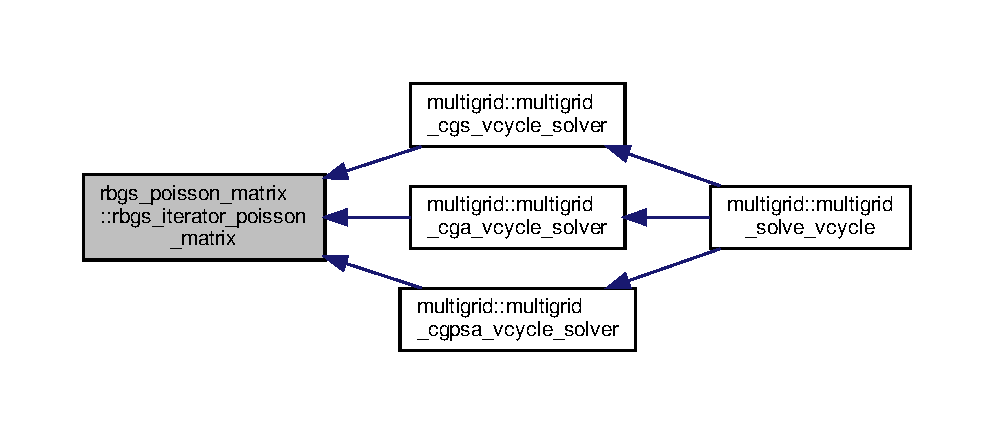
\includegraphics[width=350pt]{namespacerbgs__poisson__matrix_a35a0647dd0b1e09cb482bde7fba2be91_icgraph}
\end{center}
\end{figure}
\mbox{\Hypertarget{namespacerbgs__poisson__matrix_a4706c96056deda74122016f5c07ba337}\label{namespacerbgs__poisson__matrix_a4706c96056deda74122016f5c07ba337}} 
\index{rbgs\+\_\+poisson\+\_\+matrix@{rbgs\+\_\+poisson\+\_\+matrix}!rbgs\+\_\+solver\+\_\+poisson\+\_\+matrix@{rbgs\+\_\+solver\+\_\+poisson\+\_\+matrix}}
\index{rbgs\+\_\+solver\+\_\+poisson\+\_\+matrix@{rbgs\+\_\+solver\+\_\+poisson\+\_\+matrix}!rbgs\+\_\+poisson\+\_\+matrix@{rbgs\+\_\+poisson\+\_\+matrix}}
\subsubsection{\texorpdfstring{rbgs\+\_\+solver\+\_\+poisson\+\_\+matrix()}{rbgs\_solver\_poisson\_matrix()}}
{\footnotesize\ttfamily subroutine, public rbgs\+\_\+poisson\+\_\+matrix\+::rbgs\+\_\+solver\+\_\+poisson\+\_\+matrix (\begin{DoxyParamCaption}\item[{real(kind=8), dimension(0\+:,0\+:,0\+:), intent(inout)}]{sol,  }\item[{type(\hyperlink{structmatrix_1_1matrix__heptadiagonal}{matrix\+\_\+heptadiagonal}), intent(in)}]{a\+\_\+poisson,  }\item[{real(kind=8), dimension(0\+:,0\+:,0\+:), intent(in)}]{rhs,  }\item[{type(\hyperlink{structgeometry_1_1subdomain}{subdomain}), intent(in)}]{dm,  }\item[{integer(kind=4), intent(in)}]{maxiteration,  }\item[{real(kind=8), intent(in)}]{tolerance,  }\item[{real(kind=8), intent(in)}]{omega,  }\item[{logical, dimension(0\+:2), intent(in)}]{is\+\_\+aggregated }\end{DoxyParamCaption})}



Red-\/black Gauss-\/\+Seidel solver with convergence criteria. 


\begin{DoxyParams}{Parameters}
{\em sol} & Result solution having a shape of 3D matrix \\
\hline
{\em a\+\_\+poisson} & Heptadiagonal poisson matrix \\
\hline
{\em rhs} & R\+HS vector having a shape of 3D matrix \\
\hline
{\em dm} & Subdomain \\
\hline
{\em maxiteration} & Maximum number of iterations \\
\hline
{\em tolerance} & Convergence criteria \\
\hline
{\em omega} & Relexation factor \\
\hline
{\em is\+\_\+aggregated} & Boolean whether domain is aggregated (.true.) or not (.false.) \\
\hline
\end{DoxyParams}
Here is the call graph for this function\+:
\nopagebreak
\begin{figure}[H]
\begin{center}
\leavevmode
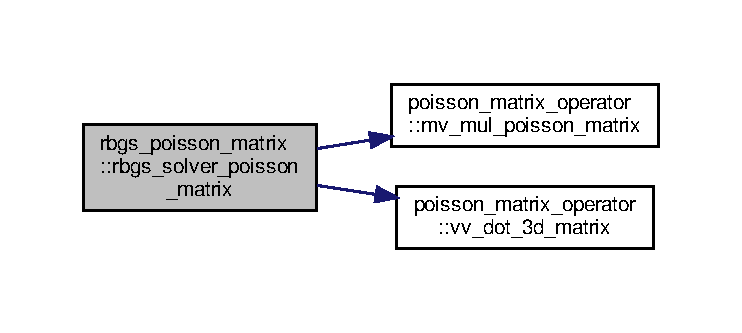
\includegraphics[width=350pt]{namespacerbgs__poisson__matrix_a4706c96056deda74122016f5c07ba337_cgraph}
\end{center}
\end{figure}
Here is the caller graph for this function\+:
\nopagebreak
\begin{figure}[H]
\begin{center}
\leavevmode
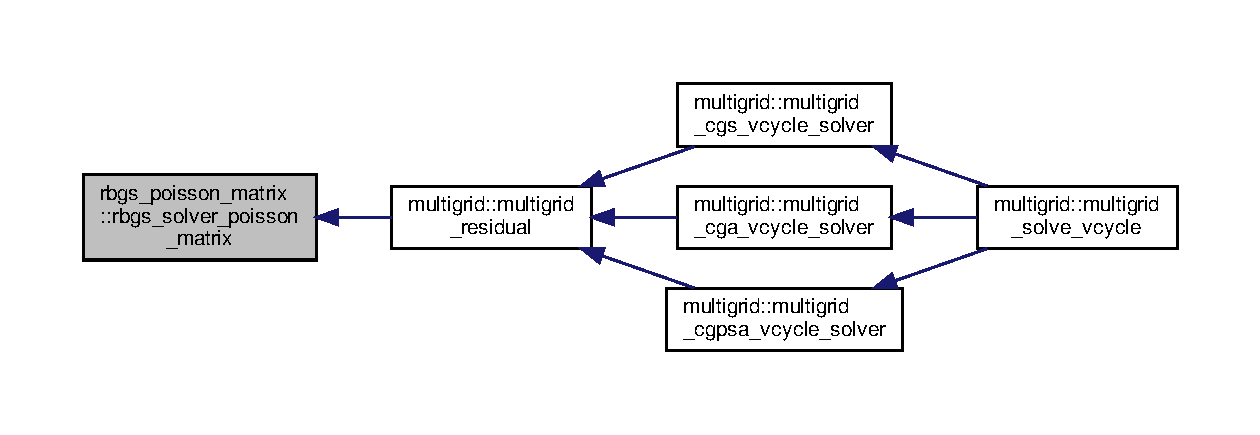
\includegraphics[width=350pt]{namespacerbgs__poisson__matrix_a4706c96056deda74122016f5c07ba337_icgraph}
\end{center}
\end{figure}

\chapter{Data Type Documentation}
\hypertarget{structmpi__topology_1_1cart__comm__1d}{}\section{mpi\+\_\+topology\+:\+:cart\+\_\+comm\+\_\+1d Type Reference}
\label{structmpi__topology_1_1cart__comm__1d}\index{mpi\+\_\+topology\+::cart\+\_\+comm\+\_\+1d@{mpi\+\_\+topology\+::cart\+\_\+comm\+\_\+1d}}


Type variable for the information of 1D communicator.  


\subsection*{Public Attributes}
\begin{DoxyCompactItemize}
\item 
\mbox{\Hypertarget{structmpi__topology_1_1cart__comm__1d_af8e266e09b59c9feb0192d6a045f5e25}\label{structmpi__topology_1_1cart__comm__1d_af8e266e09b59c9feb0192d6a045f5e25}} 
integer(kind=4) \hyperlink{structmpi__topology_1_1cart__comm__1d_af8e266e09b59c9feb0192d6a045f5e25}{myrank}
\begin{DoxyCompactList}\small\item\em Rank ID in current communicator. \end{DoxyCompactList}\item 
\mbox{\Hypertarget{structmpi__topology_1_1cart__comm__1d_a7272e89eb5b98625a78eedbdbe3eccab}\label{structmpi__topology_1_1cart__comm__1d_a7272e89eb5b98625a78eedbdbe3eccab}} 
integer(kind=4) \hyperlink{structmpi__topology_1_1cart__comm__1d_a7272e89eb5b98625a78eedbdbe3eccab}{nprocs}
\begin{DoxyCompactList}\small\item\em Number of processes in current communicator. \end{DoxyCompactList}\item 
\mbox{\Hypertarget{structmpi__topology_1_1cart__comm__1d_a6bbcb66907f7a4ac4aca5c6821205652}\label{structmpi__topology_1_1cart__comm__1d_a6bbcb66907f7a4ac4aca5c6821205652}} 
integer(kind=4) \hyperlink{structmpi__topology_1_1cart__comm__1d_a6bbcb66907f7a4ac4aca5c6821205652}{west\+\_\+rank}
\begin{DoxyCompactList}\small\item\em Previous rank ID in current communicator. \end{DoxyCompactList}\item 
\mbox{\Hypertarget{structmpi__topology_1_1cart__comm__1d_a7895ca5472496774a4ec59055dd310b1}\label{structmpi__topology_1_1cart__comm__1d_a7895ca5472496774a4ec59055dd310b1}} 
integer(kind=4) \hyperlink{structmpi__topology_1_1cart__comm__1d_a7895ca5472496774a4ec59055dd310b1}{east\+\_\+rank}
\begin{DoxyCompactList}\small\item\em Next rank ID in current communicator. \end{DoxyCompactList}\item 
\mbox{\Hypertarget{structmpi__topology_1_1cart__comm__1d_ae5e048f71450f5413a11c1d0f4c6a918}\label{structmpi__topology_1_1cart__comm__1d_ae5e048f71450f5413a11c1d0f4c6a918}} 
integer(kind=4) \hyperlink{structmpi__topology_1_1cart__comm__1d_ae5e048f71450f5413a11c1d0f4c6a918}{mpi\+\_\+comm}
\begin{DoxyCompactList}\small\item\em Current communicator. \end{DoxyCompactList}\end{DoxyCompactItemize}


\subsection{Detailed Description}
Type variable for the information of 1D communicator. 

The documentation for this type was generated from the following file\+:\begin{DoxyCompactItemize}
\item 
/home/jihoon/\+Develop/\+P\+E\+P\+S\+\_\+\+M\+G/src/\hyperlink{mpi__topology_8f90}{mpi\+\_\+topology.\+f90}\end{DoxyCompactItemize}

\hypertarget{structgeometry_1_1domain}{}\section{geometry\+:\+:domain Type Reference}
\label{structgeometry_1_1domain}\index{geometry\+::domain@{geometry\+::domain}}


Global domain information.  


\subsection*{Public Attributes}
\textbf{ }\par
\begin{DoxyCompactItemize}
\item 
\mbox{\Hypertarget{structgeometry_1_1domain_a3569446a72ab2191992294f16315edf1}\label{structgeometry_1_1domain_a3569446a72ab2191992294f16315edf1}} 
integer(kind=4) \hyperlink{structgeometry_1_1domain_a3569446a72ab2191992294f16315edf1}{nx}
\begin{DoxyCompactList}\small\item\em Number of grids in the global domain. \end{DoxyCompactList}\item 
\mbox{\Hypertarget{structgeometry_1_1domain_aadb56ae70277efeb96d8552e7d19b694}\label{structgeometry_1_1domain_aadb56ae70277efeb96d8552e7d19b694}} 
integer(kind=4) {\bfseries ny}
\item 
\mbox{\Hypertarget{structgeometry_1_1domain_aa92f4b4c069ce0a2544e2222ca0b0594}\label{structgeometry_1_1domain_aa92f4b4c069ce0a2544e2222ca0b0594}} 
integer(kind=4) {\bfseries nz}
\end{DoxyCompactItemize}

\textbf{ }\par
\begin{DoxyCompactItemize}
\item 
\mbox{\Hypertarget{structgeometry_1_1domain_a8897d7f377fd3fd5853405e5c9692d12}\label{structgeometry_1_1domain_a8897d7f377fd3fd5853405e5c9692d12}} 
real(kind=8) \hyperlink{structgeometry_1_1domain_a8897d7f377fd3fd5853405e5c9692d12}{lx}
\begin{DoxyCompactList}\small\item\em Physical length of the global domain. \end{DoxyCompactList}\item 
\mbox{\Hypertarget{structgeometry_1_1domain_a7c1f54c66cde6b0ec541b2f7846229a8}\label{structgeometry_1_1domain_a7c1f54c66cde6b0ec541b2f7846229a8}} 
real(kind=8) {\bfseries ly}
\item 
\mbox{\Hypertarget{structgeometry_1_1domain_aebbb0cfc027eec3f9eaafed12dfd9fdb}\label{structgeometry_1_1domain_aebbb0cfc027eec3f9eaafed12dfd9fdb}} 
real(kind=8) {\bfseries lz}
\end{DoxyCompactItemize}

\textbf{ }\par
\begin{DoxyCompactItemize}
\item 
\mbox{\Hypertarget{structgeometry_1_1domain_aecb690de419cdff12180b6c73aa87daf}\label{structgeometry_1_1domain_aecb690de419cdff12180b6c73aa87daf}} 
real(kind=8) \hyperlink{structgeometry_1_1domain_aecb690de419cdff12180b6c73aa87daf}{ox}
\begin{DoxyCompactList}\small\item\em Starting coordinates of the global domain. (x0, y0, z0) \end{DoxyCompactList}\item 
\mbox{\Hypertarget{structgeometry_1_1domain_a1e4a155922f64d3b2f95efbb93cfa570}\label{structgeometry_1_1domain_a1e4a155922f64d3b2f95efbb93cfa570}} 
real(kind=8) {\bfseries oy}
\item 
\mbox{\Hypertarget{structgeometry_1_1domain_acdd00f08acd1037a5b4eff090c3a19d1}\label{structgeometry_1_1domain_acdd00f08acd1037a5b4eff090c3a19d1}} 
real(kind=8) {\bfseries oz}
\end{DoxyCompactItemize}

\textbf{ }\par
\begin{DoxyCompactItemize}
\item 
\mbox{\Hypertarget{structgeometry_1_1domain_a51f16943b22e5acab127f91248fca50b}\label{structgeometry_1_1domain_a51f16943b22e5acab127f91248fca50b}} 
real(kind=8), dimension(\+:), allocatable \hyperlink{structgeometry_1_1domain_a51f16943b22e5acab127f91248fca50b}{dxm}
\begin{DoxyCompactList}\small\item\em Mesh (cell) size in each dimension. \end{DoxyCompactList}\item 
\mbox{\Hypertarget{structgeometry_1_1domain_a6e0e0af9dca8a54dfe4d5aab0e85ba75}\label{structgeometry_1_1domain_a6e0e0af9dca8a54dfe4d5aab0e85ba75}} 
real(kind=8), dimension(\+:), allocatable {\bfseries dym}
\item 
\mbox{\Hypertarget{structgeometry_1_1domain_ae33cc4a55efbe7f1dc0eded6c73aa4b3}\label{structgeometry_1_1domain_ae33cc4a55efbe7f1dc0eded6c73aa4b3}} 
real(kind=8), dimension(\+:), allocatable {\bfseries dzm}
\end{DoxyCompactItemize}

\textbf{ }\par
\begin{DoxyCompactItemize}
\item 
\mbox{\Hypertarget{structgeometry_1_1domain_a8c14a8b59fb785d4b2269dc8076da6da}\label{structgeometry_1_1domain_a8c14a8b59fb785d4b2269dc8076da6da}} 
real(kind=8), dimension(\+:), allocatable \hyperlink{structgeometry_1_1domain_a8c14a8b59fb785d4b2269dc8076da6da}{dxg}
\begin{DoxyCompactList}\small\item\em Space between grid points. \end{DoxyCompactList}\item 
\mbox{\Hypertarget{structgeometry_1_1domain_ace85559dc512416edb86321ab9c114e4}\label{structgeometry_1_1domain_ace85559dc512416edb86321ab9c114e4}} 
real(kind=8), dimension(\+:), allocatable {\bfseries dyg}
\item 
\mbox{\Hypertarget{structgeometry_1_1domain_a3fb6344986301deb02c4cae52b0e4cd3}\label{structgeometry_1_1domain_a3fb6344986301deb02c4cae52b0e4cd3}} 
real(kind=8), dimension(\+:), allocatable {\bfseries dzg}
\end{DoxyCompactItemize}

\textbf{ }\par
\begin{DoxyCompactItemize}
\item 
\mbox{\Hypertarget{structgeometry_1_1domain_ae361f615bcd5fe5d4d8046ad04a32d2b}\label{structgeometry_1_1domain_ae361f615bcd5fe5d4d8046ad04a32d2b}} 
real(kind=8), dimension(\+:), allocatable \hyperlink{structgeometry_1_1domain_ae361f615bcd5fe5d4d8046ad04a32d2b}{xg}
\begin{DoxyCompactList}\small\item\em Coordinates of grid pointss. \end{DoxyCompactList}\item 
\mbox{\Hypertarget{structgeometry_1_1domain_a2a98fddcd9b8f316d4a9bd5bd5fac39f}\label{structgeometry_1_1domain_a2a98fddcd9b8f316d4a9bd5bd5fac39f}} 
real(kind=8), dimension(\+:), allocatable {\bfseries yg}
\item 
\mbox{\Hypertarget{structgeometry_1_1domain_aca2383065957f2968b9261eccd000c3c}\label{structgeometry_1_1domain_aca2383065957f2968b9261eccd000c3c}} 
real(kind=8), dimension(\+:), allocatable {\bfseries zg}
\end{DoxyCompactItemize}

\textbf{ }\par
\begin{DoxyCompactItemize}
\item 
\mbox{\Hypertarget{structgeometry_1_1domain_a7f5ef8616243a13ec432ec9077ea1d0a}\label{structgeometry_1_1domain_a7f5ef8616243a13ec432ec9077ea1d0a}} 
logical, dimension(0\+:2) \hyperlink{structgeometry_1_1domain_a7f5ef8616243a13ec432ec9077ea1d0a}{is\+\_\+periodic}
\begin{DoxyCompactList}\small\item\em Periodic boundary condition\+: .true. if periodic, .false. if not. \end{DoxyCompactList}\end{DoxyCompactItemize}



\subsection{Detailed Description}
Global domain information. 

It contains the geometry of global domain in three-\/dimensional Cartesian cooridnates. Dimensions of grids and meshes are included. Cell-\/centered grid system is employed. 

The documentation for this type was generated from the following file\+:\begin{DoxyCompactItemize}
\item 
/home/jihoon/\+Develop/\+P\+E\+P\+S\+\_\+\+M\+G/src/geometry.\+f90\end{DoxyCompactItemize}

\hypertarget{structmatrix_1_1matrix__heptadiagonal}{}\section{matrix\+:\+:matrix\+\_\+heptadiagonal Type Reference}
\label{structmatrix_1_1matrix__heptadiagonal}\index{matrix\+::matrix\+\_\+heptadiagonal@{matrix\+::matrix\+\_\+heptadiagonal}}


Heptadiagonam matrix for finite difference method with 7-\/stencil points.  


\subsection*{Public Attributes}
\begin{DoxyCompactItemize}
\item 
\mbox{\Hypertarget{structmatrix_1_1matrix__heptadiagonal_a8e4e9d79c193e6f1c84ca92bcdec20d5}\label{structmatrix_1_1matrix__heptadiagonal_a8e4e9d79c193e6f1c84ca92bcdec20d5}} 
integer(kind=4) \hyperlink{structmatrix_1_1matrix__heptadiagonal_a8e4e9d79c193e6f1c84ca92bcdec20d5}{dof}
\begin{DoxyCompactList}\small\item\em Degree of freedom, nx$\ast$ny$\ast$nz. \end{DoxyCompactList}\item 
\mbox{\Hypertarget{structmatrix_1_1matrix__heptadiagonal_a9c13c717e99078c79ac99dec1b563a6d}\label{structmatrix_1_1matrix__heptadiagonal_a9c13c717e99078c79ac99dec1b563a6d}} 
real(kind=8), dimension(\+:,\+:,\+:,\+:), allocatable \hyperlink{structmatrix_1_1matrix__heptadiagonal_a9c13c717e99078c79ac99dec1b563a6d}{coeff}
\begin{DoxyCompactList}\small\item\em Coefficient matrix. Seven elements for each coordinate. \end{DoxyCompactList}\end{DoxyCompactItemize}


\subsection{Detailed Description}
Heptadiagonam matrix for finite difference method with 7-\/stencil points. 

It contains the degree of freedom (row size) and its seven coefficients for each coorinate. 

The documentation for this type was generated from the following file\+:\begin{DoxyCompactItemize}
\item 
/home/jihoon/\+Develop/\+P\+E\+P\+S\+\_\+\+M\+G/src/\hyperlink{matrix_8f90}{matrix.\+f90}\end{DoxyCompactItemize}

\hypertarget{structgeometry_1_1subdomain}{}\section{geometry\+:\+:subdomain Type Reference}
\label{structgeometry_1_1subdomain}\index{geometry\+::subdomain@{geometry\+::subdomain}}


Partitioned subdomain information.  


\subsection*{Public Attributes}
\begin{DoxyCompactItemize}
\item 
\mbox{\Hypertarget{structgeometry_1_1subdomain_aea7753c3a62cce4a5c8ca8f6bce7e965}\label{structgeometry_1_1subdomain_aea7753c3a62cce4a5c8ca8f6bce7e965}} 
real(kind=8), dimension(\+:,\+:,\+:), allocatable {\bfseries x}
\item 
\mbox{\Hypertarget{structgeometry_1_1subdomain_aeeeb5d9f5e919e5d674452cec8d790df}\label{structgeometry_1_1subdomain_aeeeb5d9f5e919e5d674452cec8d790df}} 
real(kind=8), dimension(\+:,\+:,\+:), allocatable {\bfseries solution}
\item 
\mbox{\Hypertarget{structgeometry_1_1subdomain_a701a6ba5307a85562218bc465772fa20}\label{structgeometry_1_1subdomain_a701a6ba5307a85562218bc465772fa20}} 
real(kind=8), dimension(\+:,\+:,\+:), allocatable {\bfseries variable}
\item 
\mbox{\Hypertarget{structgeometry_1_1subdomain_a98470eff2217eaa32f1169c2233a8d01}\label{structgeometry_1_1subdomain_a98470eff2217eaa32f1169c2233a8d01}} 
real(kind=8), dimension(\+:,\+:,\+:), allocatable {\bfseries in}
\item 
\mbox{\Hypertarget{structgeometry_1_1subdomain_ae9181672b7a5e402c32d45a58b05c907}\label{structgeometry_1_1subdomain_ae9181672b7a5e402c32d45a58b05c907}} 
real(kind=8), dimension(\+:,\+:,\+:), allocatable {\bfseries subdomain}
\item 
\mbox{\Hypertarget{structgeometry_1_1subdomain_a998dfed0dc2c8a52f074267ebbedbeb1}\label{structgeometry_1_1subdomain_a998dfed0dc2c8a52f074267ebbedbeb1}} 
real(kind=8), dimension(\+:,\+:,\+:), allocatable {\bfseries b}
\item 
\mbox{\Hypertarget{structgeometry_1_1subdomain_a92a7a57f937604398d2208eed5a1c39b}\label{structgeometry_1_1subdomain_a92a7a57f937604398d2208eed5a1c39b}} 
real(kind=8), dimension(\+:,\+:,\+:), allocatable {\bfseries rhs}
\item 
\mbox{\Hypertarget{structgeometry_1_1subdomain_a30c3dad173fc5e40edc8b540a71083c5}\label{structgeometry_1_1subdomain_a30c3dad173fc5e40edc8b540a71083c5}} 
real(kind=8), dimension(\+:,\+:,\+:), allocatable {\bfseries r}
\item 
\mbox{\Hypertarget{structgeometry_1_1subdomain_a064448f084292cb4a38046bd276c970a}\label{structgeometry_1_1subdomain_a064448f084292cb4a38046bd276c970a}} 
real(kind=8), dimension(\+:,\+:,\+:), allocatable {\bfseries residual}
\end{DoxyCompactItemize}
\textbf{ }\par
\begin{DoxyCompactItemize}
\item 
\mbox{\Hypertarget{structgeometry_1_1subdomain_afb731bbe46ffad6a0325785e65f3d299}\label{structgeometry_1_1subdomain_afb731bbe46ffad6a0325785e65f3d299}} 
integer(kind=4) \hyperlink{structgeometry_1_1subdomain_afb731bbe46ffad6a0325785e65f3d299}{nx}
\begin{DoxyCompactList}\small\item\em Grid numbers in the partitioned subdomain. \end{DoxyCompactList}\item 
\mbox{\Hypertarget{structgeometry_1_1subdomain_a1d63f2ac817a7457c94e3ac595ee50be}\label{structgeometry_1_1subdomain_a1d63f2ac817a7457c94e3ac595ee50be}} 
integer(kind=4) {\bfseries ny}
\item 
\mbox{\Hypertarget{structgeometry_1_1subdomain_ad205d5faf888902b0b1efe397f312c8e}\label{structgeometry_1_1subdomain_ad205d5faf888902b0b1efe397f312c8e}} 
integer(kind=4) {\bfseries nz}
\end{DoxyCompactItemize}

\textbf{ }\par
\begin{DoxyCompactItemize}
\item 
\mbox{\Hypertarget{structgeometry_1_1subdomain_a1a8069b63f8022e9ac03a6f0fc1faa35}\label{structgeometry_1_1subdomain_a1a8069b63f8022e9ac03a6f0fc1faa35}} 
real(kind=8) \hyperlink{structgeometry_1_1subdomain_a1a8069b63f8022e9ac03a6f0fc1faa35}{lx}
\begin{DoxyCompactList}\small\item\em Physical length of the subdomain. \end{DoxyCompactList}\item 
\mbox{\Hypertarget{structgeometry_1_1subdomain_acef77f76f536d1fbaff0263eb78f2dc5}\label{structgeometry_1_1subdomain_acef77f76f536d1fbaff0263eb78f2dc5}} 
real(kind=8) {\bfseries ly}
\item 
\mbox{\Hypertarget{structgeometry_1_1subdomain_a43705705a2aade6c23adcf7fea50c9ee}\label{structgeometry_1_1subdomain_a43705705a2aade6c23adcf7fea50c9ee}} 
real(kind=8) {\bfseries lz}
\end{DoxyCompactItemize}

\textbf{ }\par
\begin{DoxyCompactItemize}
\item 
\mbox{\Hypertarget{structgeometry_1_1subdomain_acc63b708a9901604f9212ecf25339e37}\label{structgeometry_1_1subdomain_acc63b708a9901604f9212ecf25339e37}} 
real(kind=8) \hyperlink{structgeometry_1_1subdomain_acc63b708a9901604f9212ecf25339e37}{ox}
\begin{DoxyCompactList}\small\item\em Starting coordinates of the subdomain domain. \end{DoxyCompactList}\item 
\mbox{\Hypertarget{structgeometry_1_1subdomain_ace0bde92488b6ef3e52f9d098816a45c}\label{structgeometry_1_1subdomain_ace0bde92488b6ef3e52f9d098816a45c}} 
real(kind=8) {\bfseries oy}
\item 
\mbox{\Hypertarget{structgeometry_1_1subdomain_ab7023adaf05009d17e10671e1ab84bfc}\label{structgeometry_1_1subdomain_ab7023adaf05009d17e10671e1ab84bfc}} 
real(kind=8) {\bfseries oz}
\end{DoxyCompactItemize}

\textbf{ }\par
\begin{DoxyCompactItemize}
\item 
\mbox{\Hypertarget{structgeometry_1_1subdomain_a45e4c4015e95da74673bdc46cb0619eb}\label{structgeometry_1_1subdomain_a45e4c4015e95da74673bdc46cb0619eb}} 
real(kind=8), dimension(\+:), allocatable \hyperlink{structgeometry_1_1subdomain_a45e4c4015e95da74673bdc46cb0619eb}{dxm}
\begin{DoxyCompactList}\small\item\em Mesh (cell) size in each dimension of subdomain. \end{DoxyCompactList}\item 
\mbox{\Hypertarget{structgeometry_1_1subdomain_a3994b06f249fd3ca731b1c6e301c062f}\label{structgeometry_1_1subdomain_a3994b06f249fd3ca731b1c6e301c062f}} 
real(kind=8), dimension(\+:), allocatable {\bfseries dym}
\item 
\mbox{\Hypertarget{structgeometry_1_1subdomain_a68e4b6568bc410870271842e7dc9f37a}\label{structgeometry_1_1subdomain_a68e4b6568bc410870271842e7dc9f37a}} 
real(kind=8), dimension(\+:), allocatable {\bfseries dzm}
\end{DoxyCompactItemize}

\textbf{ }\par
\begin{DoxyCompactItemize}
\item 
\mbox{\Hypertarget{structgeometry_1_1subdomain_a1f1a198a8a9dcf0a2cc571897a4bc0cb}\label{structgeometry_1_1subdomain_a1f1a198a8a9dcf0a2cc571897a4bc0cb}} 
real(kind=8), dimension(\+:), allocatable \hyperlink{structgeometry_1_1subdomain_a1f1a198a8a9dcf0a2cc571897a4bc0cb}{dxg}
\begin{DoxyCompactList}\small\item\em Space between grid points of subdomain. \end{DoxyCompactList}\item 
\mbox{\Hypertarget{structgeometry_1_1subdomain_ad4dfb84d28757bc3c3b9fdd07c8bd373}\label{structgeometry_1_1subdomain_ad4dfb84d28757bc3c3b9fdd07c8bd373}} 
real(kind=8), dimension(\+:), allocatable {\bfseries dyg}
\item 
\mbox{\Hypertarget{structgeometry_1_1subdomain_a6ab718cebcef3accb469924bc5d5d3c7}\label{structgeometry_1_1subdomain_a6ab718cebcef3accb469924bc5d5d3c7}} 
real(kind=8), dimension(\+:), allocatable {\bfseries dzg}
\end{DoxyCompactItemize}

\textbf{ }\par
\begin{DoxyCompactItemize}
\item 
\mbox{\Hypertarget{structgeometry_1_1subdomain_aca30707e5150e7168bd8bc1371970364}\label{structgeometry_1_1subdomain_aca30707e5150e7168bd8bc1371970364}} 
real(kind=8), dimension(\+:), allocatable \hyperlink{structgeometry_1_1subdomain_aca30707e5150e7168bd8bc1371970364}{xg}
\begin{DoxyCompactList}\small\item\em Coordinates of grid pointss of subdomain. \end{DoxyCompactList}\item 
\mbox{\Hypertarget{structgeometry_1_1subdomain_a078bcb84698ead561ca0546ba9a2e158}\label{structgeometry_1_1subdomain_a078bcb84698ead561ca0546ba9a2e158}} 
real(kind=8), dimension(\+:), allocatable {\bfseries yg}
\item 
\mbox{\Hypertarget{structgeometry_1_1subdomain_afdb6b7b2dc6bfc6587a1af1c6ac3a2f0}\label{structgeometry_1_1subdomain_afdb6b7b2dc6bfc6587a1af1c6ac3a2f0}} 
real(kind=8), dimension(\+:), allocatable {\bfseries zg}
\end{DoxyCompactItemize}

\textbf{ }\par
\begin{DoxyCompactItemize}
\item 
\mbox{\Hypertarget{structgeometry_1_1subdomain_a0f3a1589b2d2a7432226f2e6f3f34045}\label{structgeometry_1_1subdomain_a0f3a1589b2d2a7432226f2e6f3f34045}} 
logical, dimension(0\+:2) \hyperlink{structgeometry_1_1subdomain_a0f3a1589b2d2a7432226f2e6f3f34045}{is\+\_\+periodic}
\begin{DoxyCompactList}\small\item\em Periodic boundary condition\+: .true. if periodic, .false. if not. \end{DoxyCompactList}\end{DoxyCompactItemize}

\textbf{ }\par
\begin{DoxyCompactItemize}
\item 
\mbox{\Hypertarget{structgeometry_1_1subdomain_a17edfc7e8229d24f6223282092927d3e}\label{structgeometry_1_1subdomain_a17edfc7e8229d24f6223282092927d3e}} 
logical, dimension(0\+:2) \hyperlink{structgeometry_1_1subdomain_a17edfc7e8229d24f6223282092927d3e}{is\+\_\+aggregated}
\begin{DoxyCompactList}\small\item\em Indicate whether subdomain is aggregated in each direction\+: .true. if aggregated, .false. if not. \end{DoxyCompactList}\end{DoxyCompactItemize}

\textbf{ }\par
\begin{DoxyCompactItemize}
\item 
\mbox{\Hypertarget{structgeometry_1_1subdomain_af7a157d3eedb654d163f6d25253f4798}\label{structgeometry_1_1subdomain_af7a157d3eedb654d163f6d25253f4798}} 
integer(kind=4), public \hyperlink{structgeometry_1_1subdomain_af7a157d3eedb654d163f6d25253f4798}{ista}
\begin{DoxyCompactList}\small\item\em Indices of first and last grids of subdomain in x-\/direction, with regards to global domain. \end{DoxyCompactList}\item 
\mbox{\Hypertarget{structgeometry_1_1subdomain_a5b622d801fee0488b495d2e8cbac230d}\label{structgeometry_1_1subdomain_a5b622d801fee0488b495d2e8cbac230d}} 
integer(kind=4), public {\bfseries iend}
\end{DoxyCompactItemize}

\textbf{ }\par
\begin{DoxyCompactItemize}
\item 
\mbox{\Hypertarget{structgeometry_1_1subdomain_a06519313e1a87c437f9ca7e8325065d1}\label{structgeometry_1_1subdomain_a06519313e1a87c437f9ca7e8325065d1}} 
integer(kind=4), public \hyperlink{structgeometry_1_1subdomain_a06519313e1a87c437f9ca7e8325065d1}{jsta}
\begin{DoxyCompactList}\small\item\em Indices of first and last grids of subdomain in y-\/direction, with regards to global domain. \end{DoxyCompactList}\item 
\mbox{\Hypertarget{structgeometry_1_1subdomain_a7ad47076a641a35c16028c2a86e304b4}\label{structgeometry_1_1subdomain_a7ad47076a641a35c16028c2a86e304b4}} 
integer(kind=4), public {\bfseries jend}
\end{DoxyCompactItemize}

\textbf{ }\par
\begin{DoxyCompactItemize}
\item 
\mbox{\Hypertarget{structgeometry_1_1subdomain_ac83bbafe91c89c9d7c4be7df88cc3f72}\label{structgeometry_1_1subdomain_ac83bbafe91c89c9d7c4be7df88cc3f72}} 
integer(kind=4), public \hyperlink{structgeometry_1_1subdomain_ac83bbafe91c89c9d7c4be7df88cc3f72}{ksta}
\begin{DoxyCompactList}\small\item\em Indices of first and last grids of subdomain in z-\/direction, with regards to global domain. \end{DoxyCompactList}\item 
\mbox{\Hypertarget{structgeometry_1_1subdomain_a0e622a4e26eeb8b17fdf300e4d900ffb}\label{structgeometry_1_1subdomain_a0e622a4e26eeb8b17fdf300e4d900ffb}} 
integer(kind=4), public {\bfseries kend}
\end{DoxyCompactItemize}

\textbf{ }\par
\begin{DoxyCompactItemize}
\item 
\mbox{\Hypertarget{structgeometry_1_1subdomain_a47600c2cb2df3aa446b4eac99aa19dfa}\label{structgeometry_1_1subdomain_a47600c2cb2df3aa446b4eac99aa19dfa}} 
integer(kind=4), public \hyperlink{structgeometry_1_1subdomain_a47600c2cb2df3aa446b4eac99aa19dfa}{ddt\+\_\+yz\+\_\+plane\+\_\+x0}
\begin{DoxyCompactList}\small\item\em Derived datatypes for ghostcell communication in x-\/direction. \end{DoxyCompactList}\item 
\mbox{\Hypertarget{structgeometry_1_1subdomain_a36c015128564011d09b03d9d238782e3}\label{structgeometry_1_1subdomain_a36c015128564011d09b03d9d238782e3}} 
integer(kind=4), public {\bfseries ddt\+\_\+yz\+\_\+plane\+\_\+x1}
\item 
\mbox{\Hypertarget{structgeometry_1_1subdomain_aeddeabddc20c73b5190e44c316968222}\label{structgeometry_1_1subdomain_aeddeabddc20c73b5190e44c316968222}} 
integer(kind=4), public {\bfseries ddt\+\_\+yz\+\_\+plane\+\_\+xn}
\item 
\mbox{\Hypertarget{structgeometry_1_1subdomain_a98a8b88468c10ddeb72b0e24d9912c95}\label{structgeometry_1_1subdomain_a98a8b88468c10ddeb72b0e24d9912c95}} 
integer(kind=4), public {\bfseries ddt\+\_\+yz\+\_\+plane\+\_\+xn1}
\end{DoxyCompactItemize}

\textbf{ }\par
\begin{DoxyCompactItemize}
\item 
\mbox{\Hypertarget{structgeometry_1_1subdomain_aba7fdf219fd1e93e7b8fb10132ac7db7}\label{structgeometry_1_1subdomain_aba7fdf219fd1e93e7b8fb10132ac7db7}} 
integer(kind=4), public \hyperlink{structgeometry_1_1subdomain_aba7fdf219fd1e93e7b8fb10132ac7db7}{ddt\+\_\+xz\+\_\+plane\+\_\+y0}
\begin{DoxyCompactList}\small\item\em Derived datatypes for ghostcell communication in y-\/direction. \end{DoxyCompactList}\item 
\mbox{\Hypertarget{structgeometry_1_1subdomain_a28fdfffc1b152f766cb919e53da06c0d}\label{structgeometry_1_1subdomain_a28fdfffc1b152f766cb919e53da06c0d}} 
integer(kind=4), public {\bfseries ddt\+\_\+xz\+\_\+plane\+\_\+y1}
\item 
\mbox{\Hypertarget{structgeometry_1_1subdomain_af621df7823716c7951bd108925decfe2}\label{structgeometry_1_1subdomain_af621df7823716c7951bd108925decfe2}} 
integer(kind=4), public {\bfseries ddt\+\_\+xz\+\_\+plane\+\_\+yn}
\item 
\mbox{\Hypertarget{structgeometry_1_1subdomain_af0f570d4e2eb7d1043de964a815583a3}\label{structgeometry_1_1subdomain_af0f570d4e2eb7d1043de964a815583a3}} 
integer(kind=4), public {\bfseries ddt\+\_\+xz\+\_\+plane\+\_\+yn1}
\end{DoxyCompactItemize}

\textbf{ }\par
\begin{DoxyCompactItemize}
\item 
\mbox{\Hypertarget{structgeometry_1_1subdomain_aef06388b599b17f785bea869b6b1aa46}\label{structgeometry_1_1subdomain_aef06388b599b17f785bea869b6b1aa46}} 
integer(kind=4), public \hyperlink{structgeometry_1_1subdomain_aef06388b599b17f785bea869b6b1aa46}{ddt\+\_\+xy\+\_\+plane\+\_\+z0}
\begin{DoxyCompactList}\small\item\em Derived datatypes for ghostcell communication in z-\/direction. \end{DoxyCompactList}\item 
\mbox{\Hypertarget{structgeometry_1_1subdomain_a62c8f53379792dee38a81714fc7ebf3b}\label{structgeometry_1_1subdomain_a62c8f53379792dee38a81714fc7ebf3b}} 
integer(kind=4), public {\bfseries ddt\+\_\+xy\+\_\+plane\+\_\+z1}
\item 
\mbox{\Hypertarget{structgeometry_1_1subdomain_af89941f108e7136d906a11c126e060c4}\label{structgeometry_1_1subdomain_af89941f108e7136d906a11c126e060c4}} 
integer(kind=4), public {\bfseries ddt\+\_\+xy\+\_\+plane\+\_\+zn}
\item 
\mbox{\Hypertarget{structgeometry_1_1subdomain_a39515f94c67cf944dd8289abcfc077fa}\label{structgeometry_1_1subdomain_a39515f94c67cf944dd8289abcfc077fa}} 
integer(kind=4), public {\bfseries ddt\+\_\+xy\+\_\+plane\+\_\+zn1}
\end{DoxyCompactItemize}

\textbf{ }\par
\begin{DoxyCompactItemize}
\item 
\mbox{\Hypertarget{structgeometry_1_1subdomain_a6115dacee3e1f5aaf4cc70958ed7d9e8}\label{structgeometry_1_1subdomain_a6115dacee3e1f5aaf4cc70958ed7d9e8}} 
integer(kind=4), public \hyperlink{structgeometry_1_1subdomain_a6115dacee3e1f5aaf4cc70958ed7d9e8}{ddt\+\_\+inner\+\_\+domain}
\begin{DoxyCompactList}\small\item\em Derived datatypes for inner domain without ghostcell. \end{DoxyCompactList}\end{DoxyCompactItemize}

\textbf{ }\par
\begin{DoxyCompactItemize}
\item 
\mbox{\Hypertarget{structgeometry_1_1subdomain_ad4249dd7798aeeec124c9d573c8d4330}\label{structgeometry_1_1subdomain_ad4249dd7798aeeec124c9d573c8d4330}} 
logical \hyperlink{structgeometry_1_1subdomain_ad4249dd7798aeeec124c9d573c8d4330}{is\+\_\+x0\+\_\+boundary}
\begin{DoxyCompactList}\small\item\em Indicates whether the subdomain is x-\/boundary\+: .true. if at boundary, .false. if not. \end{DoxyCompactList}\item 
\mbox{\Hypertarget{structgeometry_1_1subdomain_ab3fa65e9d28568523cf8ed8f5724929a}\label{structgeometry_1_1subdomain_ab3fa65e9d28568523cf8ed8f5724929a}} 
logical {\bfseries is\+\_\+x1\+\_\+boundary}
\end{DoxyCompactItemize}

\textbf{ }\par
\begin{DoxyCompactItemize}
\item 
\mbox{\Hypertarget{structgeometry_1_1subdomain_a3d99e9e6d3d0a6fa70339d1e5e621fb4}\label{structgeometry_1_1subdomain_a3d99e9e6d3d0a6fa70339d1e5e621fb4}} 
logical \hyperlink{structgeometry_1_1subdomain_a3d99e9e6d3d0a6fa70339d1e5e621fb4}{is\+\_\+y0\+\_\+boundary}
\begin{DoxyCompactList}\small\item\em Indicates whether the subdomain is y-\/boundary\+: .true. if at boundary, .false. if not. \end{DoxyCompactList}\item 
\mbox{\Hypertarget{structgeometry_1_1subdomain_a16c4acb7f07ab53f0203be8c939ab629}\label{structgeometry_1_1subdomain_a16c4acb7f07ab53f0203be8c939ab629}} 
logical {\bfseries is\+\_\+y1\+\_\+boundary}
\end{DoxyCompactItemize}

\textbf{ }\par
\begin{DoxyCompactItemize}
\item 
\mbox{\Hypertarget{structgeometry_1_1subdomain_a6d5a0e5ffccf550662c1358390343279}\label{structgeometry_1_1subdomain_a6d5a0e5ffccf550662c1358390343279}} 
logical \hyperlink{structgeometry_1_1subdomain_a6d5a0e5ffccf550662c1358390343279}{is\+\_\+z0\+\_\+boundary}
\begin{DoxyCompactList}\small\item\em Indicates whether the subdomain is z-\/boundary\+: .true. if at boundary, .false. if not. \end{DoxyCompactList}\item 
\mbox{\Hypertarget{structgeometry_1_1subdomain_a462e04ec3b7c7bf80ff452c3d09e4fd5}\label{structgeometry_1_1subdomain_a462e04ec3b7c7bf80ff452c3d09e4fd5}} 
logical {\bfseries is\+\_\+z1\+\_\+boundary}
\end{DoxyCompactItemize}



\subsection{Detailed Description}
Partitioned subdomain information. 

It contains the geometry of subdomain in three-\/dimensional Cartesian cooridnates. Dimensions of grids and meshes are included. Cell-\/centered grid system is employed. Grid variables, solution, R\+HS and residual, is defined in this type variable. 

The documentation for this type was generated from the following file\+:\begin{DoxyCompactItemize}
\item 
/home/jihoon/\+Develop/\+P\+E\+P\+S\+\_\+\+M\+G/src/geometry.\+f90\end{DoxyCompactItemize}

\chapter{File Documentation}
\hypertarget{cg__poisson__matrix_8f90}{}\section{/home/jihoon/\+Develop/\+P\+E\+P\+S\+\_\+\+M\+G/src/cg\+\_\+poisson\+\_\+matrix.f90 File Reference}
\label{cg__poisson__matrix_8f90}\index{/home/jihoon/\+Develop/\+P\+E\+P\+S\+\_\+\+M\+G/src/cg\+\_\+poisson\+\_\+matrix.\+f90@{/home/jihoon/\+Develop/\+P\+E\+P\+S\+\_\+\+M\+G/src/cg\+\_\+poisson\+\_\+matrix.\+f90}}


This file contains a module for conjugate gradient method with heptadiagonal poisson matrix.  


\subsection*{Modules}
\begin{DoxyCompactItemize}
\item 
module \hyperlink{namespacecg__poisson__matrix}{cg\+\_\+poisson\+\_\+matrix}
\begin{DoxyCompactList}\small\item\em Module for for conjugate gradient method with heptadiagonal poisson matrix. \end{DoxyCompactList}\end{DoxyCompactItemize}
\subsection*{Functions/\+Subroutines}
\begin{DoxyCompactItemize}
\item 
subroutine, public \hyperlink{namespacecg__poisson__matrix_a4762a692c1b2dd5070d070e90a30e8cd}{cg\+\_\+poisson\+\_\+matrix\+::cg\+\_\+solver\+\_\+poisson\+\_\+matrix} (sol, a\+\_\+poisson, rhs, dm, maxiteration, tolerance, is\+\_\+aggregated)
\begin{DoxyCompactList}\small\item\em Conjugate gradient solver with convergence criteria. \end{DoxyCompactList}\item 
subroutine, public \hyperlink{namespacecg__poisson__matrix_a558093032b9b1f54bf1bde7bfa847829}{cg\+\_\+poisson\+\_\+matrix\+::cg\+\_\+iterator\+\_\+poisson\+\_\+matrix} (sol, a\+\_\+poisson, rhs, dm, maxiteration, is\+\_\+aggregated)
\begin{DoxyCompactList}\small\item\em Conjugate gradient iterator with number of iteration. \end{DoxyCompactList}\end{DoxyCompactItemize}


\subsection{Detailed Description}
This file contains a module for conjugate gradient method with heptadiagonal poisson matrix. 

This file contains a module for conjugate gradient solver with convergence criteria and conjugate gradient iterator with iteration number \begin{DoxyAuthor}{Author}

\begin{DoxyItemize}
\item Ji-\/\+Hoon Kang (\href{mailto:jhkang@kisti.re.kr}{\tt jhkang@kisti.\+re.\+kr}), Korea Institute of Science and Technology Information
\end{DoxyItemize}
\end{DoxyAuthor}
\begin{DoxyDate}{Date}
May 2021 
\end{DoxyDate}
\begin{DoxyVersion}{Version}
1.\+0 
\end{DoxyVersion}
\begin{DoxyParagraph}{Copyright}
Copyright (c) 2021 Ji-\/\+Hoon Kang, Korea Institute of Science and Technology Information, All rights reserved. 
\end{DoxyParagraph}
\begin{DoxyParagraph}{License }
This project is release under the terms of the M\+IT License (see L\+I\+C\+E\+N\+SE in ) 
\end{DoxyParagraph}

\hypertarget{matrix_8f90}{}\section{/home/jihoon/\+Develop/\+P\+E\+P\+S\+\_\+\+M\+G/src/matrix.f90 File Reference}
\label{matrix_8f90}\index{/home/jihoon/\+Develop/\+P\+E\+P\+S\+\_\+\+M\+G/src/matrix.\+f90@{/home/jihoon/\+Develop/\+P\+E\+P\+S\+\_\+\+M\+G/src/matrix.\+f90}}


This file contains a module that defines a matrix type.  


\subsection*{Data Types}
\begin{DoxyCompactItemize}
\item 
type \hyperlink{structmatrix_1_1matrix__heptadiagonal}{matrix\+::matrix\+\_\+heptadiagonal}
\begin{DoxyCompactList}\small\item\em Heptadiagonam matrix for finite difference method with 7-\/stencil points. \end{DoxyCompactList}\end{DoxyCompactItemize}
\subsection*{Modules}
\begin{DoxyCompactItemize}
\item 
module \hyperlink{namespacematrix}{matrix}
\begin{DoxyCompactList}\small\item\em Module for matrix type for finite difference method with 7-\/stencil points. \end{DoxyCompactList}\end{DoxyCompactItemize}
\subsection*{Functions/\+Subroutines}
\begin{DoxyCompactItemize}
\item 
subroutine \hyperlink{namespacematrix_af96fcc5a5c79a720967847d6569ce479}{matrix\+::matrix\+\_\+heptadiagonal\+\_\+create} (a\+\_\+poisson, sdm)
\begin{DoxyCompactList}\small\item\em Create the heptadiagonal matrix for finite difference method with 7-\/stencil points. \end{DoxyCompactList}\item 
subroutine \hyperlink{namespacematrix_a1c201958a669deaddeb6aa76251b394f}{matrix\+::matrix\+\_\+heptadiagonal\+\_\+destroy} (a\+\_\+poisson)
\begin{DoxyCompactList}\small\item\em Destroy the heptadiagonal matrix for finite difference method with 7-\/stencil points. \end{DoxyCompactList}\end{DoxyCompactItemize}


\subsection{Detailed Description}
This file contains a module that defines a matrix type. 

Heptadiagonal matrix supported for finite difference method using 7-\/stencil points \begin{DoxyAuthor}{Author}

\begin{DoxyItemize}
\item Ji-\/\+Hoon Kang (\href{mailto:jhkang@kisti.re.kr}{\tt jhkang@kisti.\+re.\+kr}), Korea Institute of Science and Technology Information
\end{DoxyItemize}
\end{DoxyAuthor}
\begin{DoxyDate}{Date}
May 2021 
\end{DoxyDate}
\begin{DoxyVersion}{Version}
1.\+0 
\end{DoxyVersion}
\begin{DoxyParagraph}{Copyright}
Copyright (c) 2021 Ji-\/\+Hoon Kang, Korea Institute of Science and Technology Information, All rights reserved. 
\end{DoxyParagraph}
\begin{DoxyParagraph}{License }
This project is release under the terms of the M\+IT License (see L\+I\+C\+E\+N\+SE in ) 
\end{DoxyParagraph}

\hypertarget{mpi__topology_8f90}{}\section{/home/jihoon/\+Develop/\+P\+E\+P\+S\+\_\+\+M\+G/src/mpi\+\_\+topology.f90 File Reference}
\label{mpi__topology_8f90}\index{/home/jihoon/\+Develop/\+P\+E\+P\+S\+\_\+\+M\+G/src/mpi\+\_\+topology.\+f90@{/home/jihoon/\+Develop/\+P\+E\+P\+S\+\_\+\+M\+G/src/mpi\+\_\+topology.\+f90}}


This file contains a module of communication topology for the example problem of P\+E\+P\+S\+\_\+\+MG.  


\subsection*{Data Types}
\begin{DoxyCompactItemize}
\item 
type \hyperlink{structmpi__topology_1_1cart__comm__1d}{mpi\+\_\+topology\+::cart\+\_\+comm\+\_\+1d}
\begin{DoxyCompactList}\small\item\em Type variable for the information of 1D communicator. \end{DoxyCompactList}\end{DoxyCompactItemize}
\subsection*{Modules}
\begin{DoxyCompactItemize}
\item 
module \hyperlink{namespacempi__topology}{mpi\+\_\+topology}
\begin{DoxyCompactList}\small\item\em Module for creating the cartesian topology of the M\+PI processes and subcommunicators. \end{DoxyCompactList}\end{DoxyCompactItemize}
\subsection*{Functions/\+Subroutines}
\begin{DoxyCompactItemize}
\item 
\mbox{\Hypertarget{namespacempi__topology_ae299dc83f2e6767402df3dfacfad4e44}\label{namespacempi__topology_ae299dc83f2e6767402df3dfacfad4e44}} 
subroutine, public \hyperlink{namespacempi__topology_ae299dc83f2e6767402df3dfacfad4e44}{mpi\+\_\+topology\+::mpi\+\_\+topology\+\_\+create} ()
\begin{DoxyCompactList}\small\item\em Create the cartesian topology for the M\+PI processes and subcommunicators. \end{DoxyCompactList}\item 
\mbox{\Hypertarget{namespacempi__topology_a27582d0f86406910fa43ad925ac38801}\label{namespacempi__topology_a27582d0f86406910fa43ad925ac38801}} 
subroutine, public \hyperlink{namespacempi__topology_a27582d0f86406910fa43ad925ac38801}{mpi\+\_\+topology\+::mpi\+\_\+topology\+\_\+destroy} ()
\begin{DoxyCompactList}\small\item\em Destroy the communicator for cartesian topology. \end{DoxyCompactList}\end{DoxyCompactItemize}
\subsection*{Variables}
\begin{DoxyCompactItemize}
\item 
\mbox{\Hypertarget{namespacempi__topology_a893b6fb583833278f1fd992cd4d4cbf8}\label{namespacempi__topology_a893b6fb583833278f1fd992cd4d4cbf8}} 
integer(kind=4), public \hyperlink{namespacempi__topology_a893b6fb583833278f1fd992cd4d4cbf8}{mpi\+\_\+topology\+::mpi\+\_\+world\+\_\+cart}
\begin{DoxyCompactList}\small\item\em Communicator for cartesian topology. \end{DoxyCompactList}\item 
\mbox{\Hypertarget{namespacempi__topology_af16caa219178ffc6fb90822629db8a49}\label{namespacempi__topology_af16caa219178ffc6fb90822629db8a49}} 
integer(kind=4), public {\bfseries mpi\+\_\+topology\+::nprocs}
\item 
\mbox{\Hypertarget{namespacempi__topology_a27f9bdf05c9c90f0c087aeb26b99a4f3}\label{namespacempi__topology_a27f9bdf05c9c90f0c087aeb26b99a4f3}} 
integer(kind=4), public \hyperlink{namespacempi__topology_a27f9bdf05c9c90f0c087aeb26b99a4f3}{mpi\+\_\+topology\+::myrank}
\begin{DoxyCompactList}\small\item\em Number of processes and rank ID in M\+P\+I\+\_\+\+C\+O\+M\+M\+\_\+\+W\+O\+R\+LD. \end{DoxyCompactList}\item 
\mbox{\Hypertarget{namespacempi__topology_a8f8932a2511cfd89285a6f2eb906d098}\label{namespacempi__topology_a8f8932a2511cfd89285a6f2eb906d098}} 
integer(kind=4), dimension(0\+:2), public \hyperlink{namespacempi__topology_a8f8932a2511cfd89285a6f2eb906d098}{mpi\+\_\+topology\+::np\+\_\+dim}
\begin{DoxyCompactList}\small\item\em Number of M\+PI processes in 3D topology. \end{DoxyCompactList}\item 
\mbox{\Hypertarget{namespacempi__topology_ac24cb383bdfbdf566165cf78b03677aa}\label{namespacempi__topology_ac24cb383bdfbdf566165cf78b03677aa}} 
logical, dimension(0\+:2), public \hyperlink{namespacempi__topology_ac24cb383bdfbdf566165cf78b03677aa}{mpi\+\_\+topology\+::period}
\begin{DoxyCompactList}\small\item\em Periodicity in each direction. \end{DoxyCompactList}\item 
\mbox{\Hypertarget{namespacempi__topology_a67d857c7a471473332bbfcac7682943c}\label{namespacempi__topology_a67d857c7a471473332bbfcac7682943c}} 
type(cart\+\_\+comm\+\_\+1d), target, public \hyperlink{namespacempi__topology_a67d857c7a471473332bbfcac7682943c}{mpi\+\_\+topology\+::comm\+\_\+1d\+\_\+x}
\begin{DoxyCompactList}\small\item\em Subcommunicator information in x-\/direction. \end{DoxyCompactList}\item 
\mbox{\Hypertarget{namespacempi__topology_a4f667ff8f1bbfd8075bd7629cba14c2d}\label{namespacempi__topology_a4f667ff8f1bbfd8075bd7629cba14c2d}} 
type(cart\+\_\+comm\+\_\+1d), target, public \hyperlink{namespacempi__topology_a4f667ff8f1bbfd8075bd7629cba14c2d}{mpi\+\_\+topology\+::comm\+\_\+1d\+\_\+y}
\begin{DoxyCompactList}\small\item\em Subcommunicator information in y-\/direction. \end{DoxyCompactList}\item 
\mbox{\Hypertarget{namespacempi__topology_a9d5db9f9841b438a50d1809aaf8f0efc}\label{namespacempi__topology_a9d5db9f9841b438a50d1809aaf8f0efc}} 
type(cart\+\_\+comm\+\_\+1d), target, public \hyperlink{namespacempi__topology_a9d5db9f9841b438a50d1809aaf8f0efc}{mpi\+\_\+topology\+::comm\+\_\+1d\+\_\+z}
\begin{DoxyCompactList}\small\item\em Subcommunicator information in z-\/direction. \end{DoxyCompactList}\end{DoxyCompactItemize}


\subsection{Detailed Description}
This file contains a module of communication topology for the example problem of P\+E\+P\+S\+\_\+\+MG. 

\begin{DoxyAuthor}{Author}

\begin{DoxyItemize}
\item Ji-\/\+Hoon Kang (\href{mailto:jhkang@kisti.re.kr}{\tt jhkang@kisti.\+re.\+kr}), Korea Institute of Science and Technology Information
\end{DoxyItemize}
\end{DoxyAuthor}
\begin{DoxyDate}{Date}
May 2021 
\end{DoxyDate}
\begin{DoxyVersion}{Version}
1.\+0 
\end{DoxyVersion}
\begin{DoxyParagraph}{Copyright}
Copyright (c) 2021 Ji-\/\+Hoon Kang, Korea Institute of Science and Technology Information, All rights reserved. 
\end{DoxyParagraph}
\begin{DoxyParagraph}{License }
This project is release under the terms of the M\+IT License (see L\+I\+C\+E\+N\+SE in ) 
\end{DoxyParagraph}

\hypertarget{multigrid_8f90}{}\section{/home/jihoon/\+Develop/\+P\+E\+P\+S\+\_\+\+M\+G/src/multigrid.f90 File Reference}
\label{multigrid_8f90}\index{/home/jihoon/\+Develop/\+P\+E\+P\+S\+\_\+\+M\+G/src/multigrid.\+f90@{/home/jihoon/\+Develop/\+P\+E\+P\+S\+\_\+\+M\+G/src/multigrid.\+f90}}


This file contains a module for V-\/cycle multigrid method with C\+GS, C\+GA, and C\+G\+P\+SA  C\+GS \+: Coarse grid solver without grid aggregation. C\+GA \+: Coarse grid aggregation in a target level. All grid variables are aggregated into a singel core. C\+G\+P\+SA \+: Coarse grid partial semi-\/aggregation in multiple levels.  


\subsection*{Modules}
\begin{DoxyCompactItemize}
\item 
module \hyperlink{namespacemultigrid}{multigrid}
\begin{DoxyCompactList}\small\item\em Module for solving Poisson equation with V-\/cycle multigrid(\+M\+G) method.  C\+GS, C\+GA and C\+G\+P\+SA are supported in this module. C\+GS \+: Coarse grid solver without grid aggregation. C\+GA \+: Coarse grid aggregation in a target level. All grid variables are aggregated into a singel core. C\+G\+P\+SA \+: Coarse grid partial semi-\/aggregation in multiple levels.!$>$ \end{DoxyCompactList}\end{DoxyCompactItemize}
\subsection*{Functions/\+Subroutines}
\begin{DoxyCompactItemize}
\item 
subroutine, public \hyperlink{namespacemultigrid_ac8deb32ba5698e37f75c369dc063b277}{multigrid\+::multigrid\+\_\+create} (sdm, nlevel, ncycle, aggr\+\_\+method, single\+\_\+aggr\+\_\+level, adaptive\+\_\+aggr\+\_\+level)
\begin{DoxyCompactList}\small\item\em Create MG subdomains and Poisson matrix  MG subdomain depends on aggregation type. Different subroutines are called according to aggregation type. \end{DoxyCompactList}\item 
\mbox{\Hypertarget{namespacemultigrid_a07ed47be36b2e0df9d71ec58151b642b}\label{namespacemultigrid_a07ed47be36b2e0df9d71ec58151b642b}} 
subroutine, public \hyperlink{namespacemultigrid_a07ed47be36b2e0df9d71ec58151b642b}{multigrid\+::multigrid\+\_\+destroy}
\begin{DoxyCompactList}\small\item\em Destroy all variables in all MG subdomains. \end{DoxyCompactList}\item 
subroutine \hyperlink{namespacemultigrid_a839d1e13e2d0bac4959deec5669d4171}{multigrid\+::multigrid\+\_\+prolongation\+\_\+linear\+\_\+on\+\_\+nonuniform\+\_\+grid} (val\+\_\+f, val\+\_\+c, dm\+\_\+f, dm\+\_\+c, level)
\begin{DoxyCompactList}\small\item\em Prolongation subroutine for C\+GS, C\+GA, and C\+G\+P\+SA  This subroutine is commonly used by using stride\+\_\+f and offest\+\_\+f variables Constant profile in assumed in finer level. \end{DoxyCompactList}\item 
subroutine \hyperlink{namespacemultigrid_ad1ba34848f786afdf0e91afb3d3be819}{multigrid\+::multigrid\+\_\+residual} (rsd, a\+\_\+poisson, x, rhs, dm, is\+\_\+aggregated)
\begin{DoxyCompactList}\small\item\em Residual calculation. rsd = rhs -\/ a\+\_\+poisson $\ast$ x. \end{DoxyCompactList}\item 
subroutine, public \hyperlink{namespacemultigrid_a7d60c9d01777350a79ff7bd975a90121}{multigrid\+::multigrid\+\_\+solve\+\_\+vcycle} (sol, rsd, a\+\_\+poisson, rhs, sdm, maxiteration, tolerance, omega\+\_\+sor)
\begin{DoxyCompactList}\small\item\em V-\/\+Cycle MG solver\+: call subroutines according to aggregation type. \end{DoxyCompactList}\item 
subroutine \hyperlink{namespacemultigrid_aa8278baf0276649fe656c1b8f7dba30a}{multigrid\+::multigrid\+\_\+cgs\+\_\+vcycle\+\_\+solver} (sol, rsd, a\+\_\+poisson, rhs, sdm, maxiteration, tolerance, omega\+\_\+sor)
\begin{DoxyCompactList}\small\item\em V-\/\+Cycle MG solver with C\+GS. \end{DoxyCompactList}\item 
subroutine \hyperlink{namespacemultigrid_a4295ca0af002ede1dee98750922f1f60}{multigrid\+::multigrid\+\_\+cga\+\_\+vcycle\+\_\+solver} (sol, rsd, a\+\_\+poisson, rhs, sdm, maxiteration, tolerance, omega\+\_\+sor)
\begin{DoxyCompactList}\small\item\em V-\/\+Cycle MG solver with C\+GA  M\+P\+I\+\_\+\+Gather/\+M\+P\+I\+\_\+\+Scatterv with derived datatypes are used for aggregation. \end{DoxyCompactList}\item 
subroutine \hyperlink{namespacemultigrid_ae89565627880985244634750502edab5}{multigrid\+::multigrid\+\_\+cgpsa\+\_\+vcycle\+\_\+solver} (sol, rsd, a\+\_\+poisson, rhs, sdm, maxiteration, tolerance, omega\+\_\+sor)
\begin{DoxyCompactList}\small\item\em V-\/\+Cycle MG solver with C\+G\+P\+SA  M\+P\+I\+\_\+\+Gather/\+M\+P\+I\+\_\+\+Scatterv with derived datatypes are used for aggregation. \end{DoxyCompactList}\end{DoxyCompactItemize}
\textbf{ }\par
\begin{DoxyCompactItemize}
\item 
subroutine \hyperlink{namespacemultigrid_acb52ce247bf637e69274d8da44d1f159}{multigrid\+::multigrid\+\_\+subdomain\+\_\+create\+\_\+cgs} (sdm)
\begin{DoxyCompactList}\small\item\em Create MG subdomains for C\+GS  Define MG domain and assign grid dimensions such as mesh size, grid spacing and grid coordinates in each MG levels. \end{DoxyCompactList}\end{DoxyCompactItemize}

\textbf{ }\par
\begin{DoxyCompactItemize}
\item 
subroutine \hyperlink{namespacemultigrid_ae33e2e076cc087e7d149a3150c1ca1af}{multigrid\+::multigrid\+\_\+subdomain\+\_\+create\+\_\+cga} (sdm)
\begin{DoxyCompactList}\small\item\em Create MG subdomains for C\+GA  Define MG domain and assign grid dimensions such as mesh size, grid spacing and grid coordinates in each MG levels. \end{DoxyCompactList}\end{DoxyCompactItemize}

\textbf{ }\par
\begin{DoxyCompactItemize}
\item 
subroutine \hyperlink{namespacemultigrid_aa2eb7c900fb5875f844c04c27c552373}{multigrid\+::multigrid\+\_\+subdomain\+\_\+create\+\_\+cgpsa} (sdm)
\begin{DoxyCompactList}\small\item\em Create MG subdomains for C\+G\+P\+SA  Define MG domain and assign grid dimensions such as mesh size, grid spacing and grid coordinates in each MG levels. \end{DoxyCompactList}\end{DoxyCompactItemize}



\subsection{Detailed Description}
This file contains a module for V-\/cycle multigrid method with C\+GS, C\+GA, and C\+G\+P\+SA  C\+GS \+: Coarse grid solver without grid aggregation. C\+GA \+: Coarse grid aggregation in a target level. All grid variables are aggregated into a singel core. C\+G\+P\+SA \+: Coarse grid partial semi-\/aggregation in multiple levels. 

\begin{DoxyAuthor}{Author}

\begin{DoxyItemize}
\item Ji-\/\+Hoon Kang (\href{mailto:jhkang@kisti.re.kr}{\tt jhkang@kisti.\+re.\+kr}), Korea Institute of Science and Technology Information
\end{DoxyItemize}
\end{DoxyAuthor}
\begin{DoxyDate}{Date}
May 2021 
\end{DoxyDate}
\begin{DoxyVersion}{Version}
1.\+0 
\end{DoxyVersion}
\begin{DoxyParagraph}{Copyright}
Copyright (c) 2021 Ji-\/\+Hoon Kang, Korea Institute of Science and Technology Information, All rights reserved. 
\end{DoxyParagraph}
\begin{DoxyParagraph}{License }
This project is release under the terms of the M\+IT License (see L\+I\+C\+E\+N\+SE in ) 
\end{DoxyParagraph}

\hypertarget{multigrid__debug__info_8f90}{}\section{/home/jihoon/\+Develop/\+P\+E\+P\+S\+\_\+\+M\+G/src/multigrid\+\_\+debug\+\_\+info.f90 File Reference}
\label{multigrid__debug__info_8f90}\index{/home/jihoon/\+Develop/\+P\+E\+P\+S\+\_\+\+M\+G/src/multigrid\+\_\+debug\+\_\+info.\+f90@{/home/jihoon/\+Develop/\+P\+E\+P\+S\+\_\+\+M\+G/src/multigrid\+\_\+debug\+\_\+info.\+f90}}


This file contains a module for printing multigrid information for debugging.  


\subsection*{Modules}
\begin{DoxyCompactItemize}
\item 
module \hyperlink{namespacemultigrid__debug}{multigrid\+\_\+debug}
\begin{DoxyCompactList}\small\item\em Module for printing multigrid information for debugging. \end{DoxyCompactList}\end{DoxyCompactItemize}
\subsection*{Functions/\+Subroutines}
\begin{DoxyCompactItemize}
\item 
subroutine, public \hyperlink{namespacemultigrid__debug_aa5dcd15e32c5dc719638263835c5ed43}{multigrid\+\_\+debug\+::multigrid\+\_\+debug\+\_\+print\+\_\+subdomain\+\_\+grid\+\_\+info} (sdm, mg\+\_\+sdm, n\+\_\+levels)
\begin{DoxyCompactList}\small\item\em Print the grid information. \end{DoxyCompactList}\item 
subroutine, public \hyperlink{namespacemultigrid__debug_aae55d6fc6a22d97825619d5bb58a1b88}{multigrid\+\_\+debug\+::multigrid\+\_\+debug\+\_\+print\+\_\+poisson\+\_\+matrix\+\_\+info} (mg\+\_\+sdm, mg\+\_\+a\+\_\+poisson, lv)
\begin{DoxyCompactList}\small\item\em Print the poisson matrix info in multigrid levels. \end{DoxyCompactList}\item 
subroutine, public \hyperlink{namespacemultigrid__debug_a99e36a8239b91fbf3681cd88ab8f06dd}{multigrid\+\_\+debug\+::multigrid\+\_\+debug\+\_\+print\+\_\+restriction\+\_\+info} (val\+\_\+c, val\+\_\+f, vol\+\_\+c, vol\+\_\+f, level, nx\+\_\+c, ny\+\_\+c, nz\+\_\+c, i\+\_\+stride\+\_\+f, j\+\_\+stride\+\_\+f, k\+\_\+stride\+\_\+f, i\+\_\+offset\+\_\+f, j\+\_\+offset\+\_\+f, k\+\_\+offset\+\_\+f)
\begin{DoxyCompactList}\small\item\em Print the restriction results from finer grid to coarser grid. \end{DoxyCompactList}\item 
subroutine, public \hyperlink{namespacemultigrid__debug_a4e9617a0cc65c4169970f289117de416}{multigrid\+\_\+debug\+::multigrid\+\_\+debug\+\_\+print\+\_\+prolongation\+\_\+info} (val\+\_\+c, val\+\_\+f, level, nx\+\_\+f, ny\+\_\+f, nz\+\_\+f, i\+\_\+stride\+\_\+f, j\+\_\+stride\+\_\+f, k\+\_\+stride\+\_\+f, i\+\_\+offset\+\_\+f, j\+\_\+offset\+\_\+f, k\+\_\+offset\+\_\+f)
\begin{DoxyCompactList}\small\item\em Print the prolongation results from coarser grid to finer grid. \end{DoxyCompactList}\item 
subroutine, public \hyperlink{namespacemultigrid__debug_ad5c036138c7fd5e103641a667a88e6cf}{multigrid\+\_\+debug\+::multigrid\+\_\+debug\+\_\+print\+\_\+coarsest\+\_\+level\+\_\+solution} (cyc, mg\+\_\+sdm)
\begin{DoxyCompactList}\small\item\em Print the solution in the coarsest level. \end{DoxyCompactList}\end{DoxyCompactItemize}


\subsection{Detailed Description}
This file contains a module for printing multigrid information for debugging. 

\begin{DoxyAuthor}{Author}

\begin{DoxyItemize}
\item Ji-\/\+Hoon Kang (\href{mailto:jhkang@kisti.re.kr}{\tt jhkang@kisti.\+re.\+kr}), Korea Institute of Science and Technology Information
\end{DoxyItemize}
\end{DoxyAuthor}
\begin{DoxyDate}{Date}
May 2021 
\end{DoxyDate}
\begin{DoxyVersion}{Version}
1.\+0 
\end{DoxyVersion}
\begin{DoxyParagraph}{Copyright}
Copyright (c) 2021 Ji-\/\+Hoon Kang, Korea Institute of Science and Technology Information, All rights reserved. 
\end{DoxyParagraph}
\begin{DoxyParagraph}{License }
This project is release under the terms of the M\+IT License (see L\+I\+C\+E\+N\+SE in ) 
\end{DoxyParagraph}

\hypertarget{para__range_8f90}{}\section{/home/jihoon/\+Develop/\+P\+E\+P\+S\+\_\+\+M\+G/src/para\+\_\+range.f90 File Reference}
\label{para__range_8f90}\index{/home/jihoon/\+Develop/\+P\+E\+P\+S\+\_\+\+M\+G/src/para\+\_\+range.\+f90@{/home/jihoon/\+Develop/\+P\+E\+P\+S\+\_\+\+M\+G/src/para\+\_\+range.\+f90}}


The para\+\_\+range function assigns the computing range to each M\+PI process.  


\subsection*{Functions/\+Subroutines}
\begin{DoxyCompactItemize}
\item 
subroutine \hyperlink{para__range_8f90_ab75ab386311975aa4ff7cac06798fcd4}{para\+\_\+range} (n1, n2, nprocs, myrank, ista, iend)
\begin{DoxyCompactList}\small\item\em Compute the indices of the assigned range for each M\+PI process . \end{DoxyCompactList}\end{DoxyCompactItemize}


\subsection{Detailed Description}
The para\+\_\+range function assigns the computing range to each M\+PI process. 

\begin{DoxyAuthor}{Author}

\begin{DoxyItemize}
\item Ji-\/\+Hoon Kang (\href{mailto:jhkang@kisti.re.kr}{\tt jhkang@kisti.\+re.\+kr}), Korea Institute of Science and Technology Information
\end{DoxyItemize}
\end{DoxyAuthor}
\begin{DoxyDate}{Date}
May 2021 
\end{DoxyDate}
\begin{DoxyVersion}{Version}
1.\+0 
\end{DoxyVersion}
\begin{DoxyParagraph}{Copyright}
Copyright (c) 2021 Ji-\/\+Hoon Kang, Korea Institute of Science and Technology Information, All rights reserved. 
\end{DoxyParagraph}
\begin{DoxyParagraph}{License }
This project is release under the terms of the M\+IT License (see L\+I\+C\+E\+N\+SE in ) 
\end{DoxyParagraph}


\subsection{Function/\+Subroutine Documentation}
\mbox{\Hypertarget{para__range_8f90_ab75ab386311975aa4ff7cac06798fcd4}\label{para__range_8f90_ab75ab386311975aa4ff7cac06798fcd4}} 
\index{para\+\_\+range.\+f90@{para\+\_\+range.\+f90}!para\+\_\+range@{para\+\_\+range}}
\index{para\+\_\+range@{para\+\_\+range}!para\+\_\+range.\+f90@{para\+\_\+range.\+f90}}
\subsubsection{\texorpdfstring{para\+\_\+range()}{para\_range()}}
{\footnotesize\ttfamily subroutine para\+\_\+range (\begin{DoxyParamCaption}\item[{integer(kind=4), intent(in)}]{n1,  }\item[{integer(kind=4), intent(in)}]{n2,  }\item[{integer(kind=4), intent(in)}]{nprocs,  }\item[{integer(kind=4), intent(in)}]{myrank,  }\item[{integer(kind=4), intent(out)}]{ista,  }\item[{integer(kind=4), intent(out)}]{iend }\end{DoxyParamCaption})}



Compute the indices of the assigned range for each M\+PI process . 


\begin{DoxyParams}{Parameters}
{\em n1} & First index of total range \\
\hline
{\em n2} & Last index of total range \\
\hline
{\em nprocs} & Number of M\+PI process \\
\hline
{\em myrank} & Rank ID of my M\+PI process \\
\hline
{\em ista} & First index of assigned range for myrank \\
\hline
{\em iend} & Last index of assigned range for myrank \\
\hline
\end{DoxyParams}
Here is the caller graph for this function\+:
\nopagebreak
\begin{figure}[H]
\begin{center}
\leavevmode
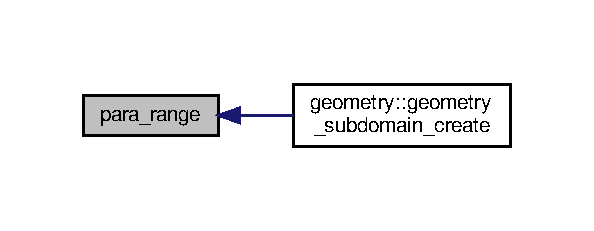
\includegraphics[width=285pt]{para__range_8f90_ab75ab386311975aa4ff7cac06798fcd4_icgraph}
\end{center}
\end{figure}

\hypertarget{poisson__matrix__operator_8f90}{}\section{/home/jihoon/\+Develop/\+P\+E\+P\+S\+\_\+\+M\+G/src/poisson\+\_\+matrix\+\_\+operator.f90 File Reference}
\label{poisson__matrix__operator_8f90}\index{/home/jihoon/\+Develop/\+P\+E\+P\+S\+\_\+\+M\+G/src/poisson\+\_\+matrix\+\_\+operator.\+f90@{/home/jihoon/\+Develop/\+P\+E\+P\+S\+\_\+\+M\+G/src/poisson\+\_\+matrix\+\_\+operator.\+f90}}


This file contains a module that conducts matrix operations of heptadiagonal poisson matrix.  


\subsection*{Modules}
\begin{DoxyCompactItemize}
\item 
module \hyperlink{namespacepoisson__matrix__operator}{poisson\+\_\+matrix\+\_\+operator}
\begin{DoxyCompactList}\small\item\em Module for matrix operations of heptadiagonal poisson matrix. \end{DoxyCompactList}\end{DoxyCompactItemize}
\subsection*{Functions/\+Subroutines}
\begin{DoxyCompactItemize}
\item 
subroutine, public \hyperlink{namespacepoisson__matrix__operator_a10219d15282e48b5afab88408912fb2f}{poisson\+\_\+matrix\+\_\+operator\+::vv\+\_\+dot\+\_\+3d\+\_\+matrix} (result, x, y, nx, ny, nz, is\+\_\+serial)
\begin{DoxyCompactList}\small\item\em Inner product for 3D matrix x and 3D matrix y. A 3D matrix is treated as a vector. \end{DoxyCompactList}\item 
subroutine, public \hyperlink{namespacepoisson__matrix__operator_a0a0591ff6a44595b830d4d0655e25106}{poisson\+\_\+matrix\+\_\+operator\+::mv\+\_\+mul\+\_\+poisson\+\_\+matrix} (y, a\+\_\+poisson, x, dm, is\+\_\+serial)
\begin{DoxyCompactList}\small\item\em MV multiplication for heptadiagonal poisson matrix a\+\_\+poisson and 3D matrix x 3D matrix is treated as a vector and poisson matrix is treated as a matrix. \end{DoxyCompactList}\end{DoxyCompactItemize}


\subsection{Detailed Description}
This file contains a module that conducts matrix operations of heptadiagonal poisson matrix. 

The operations contains MV multiplication and VV inner product \begin{DoxyAuthor}{Author}

\begin{DoxyItemize}
\item Ji-\/\+Hoon Kang (\href{mailto:jhkang@kisti.re.kr}{\tt jhkang@kisti.\+re.\+kr}), Korea Institute of Science and Technology Information
\end{DoxyItemize}
\end{DoxyAuthor}
\begin{DoxyDate}{Date}
May 2021 
\end{DoxyDate}
\begin{DoxyVersion}{Version}
1.\+0 
\end{DoxyVersion}
\begin{DoxyParagraph}{Copyright}
Copyright (c) 2021 Ji-\/\+Hoon Kang, Korea Institute of Science and Technology Information, All rights reserved. 
\end{DoxyParagraph}
\begin{DoxyParagraph}{License }
This project is release under the terms of the M\+IT License (see L\+I\+C\+E\+N\+SE in ) 
\end{DoxyParagraph}

\hypertarget{rbgs__poisson__matrix_8f90}{}\section{/home/jihoon/\+Develop/\+P\+E\+P\+S\+\_\+\+M\+G/src/rbgs\+\_\+poisson\+\_\+matrix.f90 File Reference}
\label{rbgs__poisson__matrix_8f90}\index{/home/jihoon/\+Develop/\+P\+E\+P\+S\+\_\+\+M\+G/src/rbgs\+\_\+poisson\+\_\+matrix.\+f90@{/home/jihoon/\+Develop/\+P\+E\+P\+S\+\_\+\+M\+G/src/rbgs\+\_\+poisson\+\_\+matrix.\+f90}}


This file contains a module for red-\/black Gauss-\/\+Seidel method with heptadiagonal poisson matrix.  


\subsection*{Modules}
\begin{DoxyCompactItemize}
\item 
module \hyperlink{namespacerbgs__poisson__matrix}{rbgs\+\_\+poisson\+\_\+matrix}
\begin{DoxyCompactList}\small\item\em Module for for red-\/black Gauss-\/\+Seidel method with heptadiagonal poisson matrix. \end{DoxyCompactList}\end{DoxyCompactItemize}
\subsection*{Functions/\+Subroutines}
\begin{DoxyCompactItemize}
\item 
subroutine, public \hyperlink{namespacerbgs__poisson__matrix_a4706c96056deda74122016f5c07ba337}{rbgs\+\_\+poisson\+\_\+matrix\+::rbgs\+\_\+solver\+\_\+poisson\+\_\+matrix} (sol, a\+\_\+poisson, rhs, dm, maxiteration, tolerance, omega, is\+\_\+aggregated)
\begin{DoxyCompactList}\small\item\em Red-\/black Gauss-\/\+Seidel solver with convergence criteria. \end{DoxyCompactList}\item 
subroutine, public \hyperlink{namespacerbgs__poisson__matrix_a35a0647dd0b1e09cb482bde7fba2be91}{rbgs\+\_\+poisson\+\_\+matrix\+::rbgs\+\_\+iterator\+\_\+poisson\+\_\+matrix} (sol, a\+\_\+poisson, rhs, dm, maxiteration, omega, is\+\_\+aggregated)
\begin{DoxyCompactList}\small\item\em Red-\/black Gauss-\/\+Seidel solver with convergence criteria. \end{DoxyCompactList}\end{DoxyCompactItemize}


\subsection{Detailed Description}
This file contains a module for red-\/black Gauss-\/\+Seidel method with heptadiagonal poisson matrix. 

This file contains a module for red-\/black Gauss-\/\+Seidel (R\+B\+GS) solver with convergence criteria and R\+B\+GS iterator with iteration number \begin{DoxyAuthor}{Author}

\begin{DoxyItemize}
\item Ji-\/\+Hoon Kang (\href{mailto:jhkang@kisti.re.kr}{\tt jhkang@kisti.\+re.\+kr}), Korea Institute of Science and Technology Information
\end{DoxyItemize}
\end{DoxyAuthor}
\begin{DoxyDate}{Date}
May 2021 
\end{DoxyDate}
\begin{DoxyVersion}{Version}
1.\+0 
\end{DoxyVersion}
\begin{DoxyParagraph}{Copyright}
Copyright (c) 2021 Ji-\/\+Hoon Kang, Korea Institute of Science and Technology Information, All rights reserved. 
\end{DoxyParagraph}
\begin{DoxyParagraph}{License }
This project is release under the terms of the M\+IT License (see L\+I\+C\+E\+N\+SE in ) 
\end{DoxyParagraph}

%--- End generated contents ---

% Index
\backmatter
\newpage
\phantomsection
\clearemptydoublepage
\addcontentsline{toc}{chapter}{Index}
\printindex

\end{document}
